\documentclass[11pt]{article}
%\usepackage[acronym,nonumberlist,toc]{glossaries}
\usepackage{graphicx}
\usepackage{times}
\usepackage{amsmath}
\usepackage[section]{placeins}
%\usepackage{subfigure}
\usepackage{subcaption}
\usepackage{booktabs}
\usepackage[version=4]{mhchem}
\usepackage{wrapfig}
\usepackage{textcomp}
\usepackage{geometry}
\geometry{left=2.5cm,right=2.5cm,top=2.5cm,bottom=2cm}
\usepackage{multirow}
\usepackage{color}
\usepackage[sort,numbers]{natbib}
\usepackage{authblk}
\usepackage[hyphens]{url}
\usepackage[colorlinks,linkcolor=blue,anchorcolor=blue,citecolor=blue,urlcolor=blue]{hyperref}


\title{Prediction of self-healing in engineered cementitious composite: Machine learning comparative analysis}
\author{Guangwei Chen $^{1,2,*}$, Patrick Tang $^{1}$, Shuo Chen $^{1}$, Shangyong Wang $^{1}$, and Hongzhi Cui $^3$}


\affil[1]{The University of Newcastle,  Callaghan, 2308, NSW, Australia}
\affil[2]{Qiannan Normal College of Nationalities, Guizhou, China}
\affil[3]{College of Civil and Transportation Engineering, Shenzhen University, Shenzhen 518060, China}
\date{}  

\begin{document}


%
%\address{%
%	$^{1}$ \quad The University of Newcastle,  Callaghan, 2308, NSW, Australia  }
%
%
%\corres{Correspondence: guangwei.chen@uon.edu.au}
%
%
%% Abstract (Do not insert blank lines, i.e. \\) 
%\abstract{Engineered cementitious composite (ECC) is a unique material which can significantly contribute to self-heal cracks based on ongoing hydration \cite{yildirim2014influence}. As model-free approaches eliminating the need of new models for different prediction problems, machine learning algorithms have been widely used to model the properties of concrete. This paper aims to provide a comparative analysis on the performance of machine learning models, the individual and ensemble methods, in predicting self-healing capability of ECC. These models include four individual methods (linear regression (LR), back-propagation neural network (BPNN), classification and regression tree (CRAT), and support vector regression(SVR)), three ensemble methods (bagging, AdaBoost, and stacking) with each of the four individual models used as the based learner. The results shows that the stacking model performs the best with the lowest error and highest accuracy on the self-healing capability prediction of ECC. On average, all ensemble models improve the prediction performance of the individual model which is used as the base learner in the ensemble model. }

% Keywords
%\keyword{ECC, self-healing, machine learning, ensemble method}
\maketitle

\begin{abstract}
	Engineered cementitious composite (ECC) is a unique material which can significantly contribute to self-healing behaviour based on ongoing hydration. However, it's difficult to model and predict the self-healing effect of ECC. Although different machine learning (ML) algorithms have been utilized to predict several properties of concrete, the application of ML on self-healing prediction is considerably rare. This paper aims to provide a comparative analysis on the performance of various machine learning models in predicting self-healing capability of ECC. These models include four individual methods (linear regression (LR), back-propagation neural network (BPNN), classification and regression tree (CRAT), and support vector regression(SVR)), and three ensemble methods (bagging, AdaBoost, and stacking) with each of the four individual models used as the based learner. A series of experimental works on self-healing performance of ECC samples was conducted and the results were used to develop the ML models and compare the accuracy among the ML models. Among the individual models studied, the BPNN model performed the best in terms of RMSE and $R^2$. In general, all ensemble methods could improve the prediction performance of individual models, however the improvement varies. Among all the ML models studied including both individual and ensemble methods, the Stack LR model demonstrated the best prediction results on self-healing of ECC. The results concluded that the individual and ensemble methods can be used to predict the self-healing of ECC. However, selecting an appropriate base learner and ensemble method is critical. To improve the performance accuracy, researchers should employ different ensemble methods to compare their effectiveness with different ML models.
\end{abstract}

\smallskip
\noindent \textbf{Keywords } ECC, self-healing, machine learning, ensemble method

	\section{Introduction}
	
	According to a research project commissioned by Materials for Life (M4L), the issues associated with cracking in concrete experienced by clients, design team members and contractors were more than any other problems \cite{gardner2018survey}. Moreover, cracks are primarily responsible for the reduction of strength and stiffness of concrete. In European countries, the annual cost spent on maintenance, refurbishment, and repair of concrete cracks in prolonging the service life of infrastructure is estimated around 50\% of their annual construction budget \cite{cailleux2009investigations}. It has been suggested by M4L that self-healing cementitious materials is of great potential to address the problems associated with concrete cracking and reduce the maintenance costs over a structure’s lifetime \cite{gardner2018survey}.
	
% 	A market research project was commissioned by Materials for Life (M4L), which shows cracking damage in concrete was experienced more than any other problems \cite{gardner2018survey}. Moreover, cracks are primarily responsible for the reduction of the strength and stiffness of the concrete structure. Annual cost spent on maintenance, refurbishment and repair such cracks to prolong the service life of infrastructure is estimated around 50\% of the annual construction budget in European \cite{cailleux2009investigations}. Based on such circumstances, self-healing cementitious materials are proposed by M4L research team. They state self-healing cementitious materials benefit water retaining infrastructure to reduce repair costs over a premium in the capital material cost \cite{gardner2018survey}. 

    The inspiration of self-healing comes from the biomimicry concept and the healing process in living nature \cite{ramadan2017modeling}. For example, the skin of humans or animals can biologically repair itself from simple injuries. In cement-based materials, the process of crack self-healing can be categorised into two major mechanisms, autogenous healing and autonomous healing \cite{tang2015robust}. The former indicates the self-healing ability resulted from the physical and/or chemical composition of the cementitious matrix, whereas the self-healing mechanism of the latter is triggered by some biological agents, such as bacteria which are deliberately introduced into the cementitious matrix.
	
% 	The inspiration of self-healing comes from biomimicry concept and the healing process in living nature \cite{ramadan2017modeling}. For example, the skin of humans or animals can biologically repair itself from scars injured area. According to the healing mechanism, self-healing can be  categorised into two major classes, autogenous healing and autonomous healing \cite{tang2015robust}. The former indicates the self-healing ability results from the physical and/or chemical composition of the cementitious matrix. And the latter states the self-healing mechanism is triggered by some biological agents, such as bacteria which are artificially presented in the cementitious matrix.

Generally, the autogenous self-healing of concrete is mainly controlled by two mechanisms including (1) further hydration of cement particles and/or swelling of calcium silicate hydrate; (2) calcium hydroxide carbonation \cite{edvardsen1999water,tang2016selfhealing}. It has been reported that the crack widths of 10$\mu$m \cite{jacobsen1995sem}, 100 $\mu$m \cite{reinhardt2003permeability}, 200 $\mu$m \cite{csahmaran2008influence}, 205 $\mu$m \cite{edvardsen1999water} and 300 $\mu$m \cite{clear1985effects} of ECC can be self-healed completely \cite{sahmaran2013self}. 
	
% 	Generally, autogenous self-healing in concrete is attributed to two major mechanisms including (1) further hydration of cement particles and/or swelling of calcium silicate hydrate; (2) calcium hydroxide carbonation \cite{edvardsen1999water,tang2016selfhealing}. Researchers have proposed the maximum crack widths as 10$\mu$m \cite{jacobsen1995sem}, 100 $\mu$m \cite{reinhardt2003permeability}, 200 $\mu$m \cite{csahmaran2008influence}, 205 $\mu$m \cite{edvardsen1999water} and 300 $\mu$m \cite{clear1985effects} are self-healed completely \cite{sahmaran2013self}. 
	
	Engineered cementitious composite (ECC) is a high performance fiber-reinforced cementitious composite and its matrix design is strongly associated with the autogenous self-healing mechanism \cite{kamada2000effects}. ECC features high tensile ductility with a typical fiber-volume fraction of 2\%  \cite{li1998innovations,ozbay2013self} to promote the self-healing ability \cite{tang2015robust}. 
	% for over 300 $\mu$m cracks
	
	However, the intrinsic self-healing ability of ECC is complex and difficult to predict because of different mineral admixture types, interactivity between different composites in the cementitious matrix and its interaction with the exposed environment \cite{wu2012review}, and unpredictable crack location, orientation and width \cite{huang2013characterization}. Previous studies have explored the influence of several factors such as limestone powders (LP) \cite{suleiman2019visualization,zhou2008developing}, fly ash (FA) \cite{li2007self,zhang2014investigating}, hydrated lime \cite{yildirim2014influence}, water/binder ratio \cite{yang2005self}, water permeation \cite{sahmaran2007transport} and different curing conditions (air, carbon dioxide, wet/dry and water) \cite{qian2010influence} on self-healing behaviour of ECC. However, the relationship between multiple factors is unclear and non-linear, so it’s difficult to predict self-healing of ECC mathematically based on the available data. Moreover, mathematical models based on empirical data are generally in regression forms, which cannot be used when the problem (e.g. prediction of self-healing potential of ECC) contains too many independent variables because of less accuracy and more assumption in the regression form (linear, non-linear, etc.) \cite{alshihri2009neural}.
	
% 	The intrinsic self-healing ability of ECC is complex and uncertain due to material nature, interactivity between different composites in the cementitious matrix and its interaction with the exposed environment \cite{wu2012review}, and unpredictable crack location, orientation and width \cite{huang2013characterization}. Several studies explored the influence of different factors, such as limestone powders (LP) \cite{suleiman2019visualization,zhou2008developing}, fly ash (FA) \cite{li2007self,zhang2014investigating}, hydrate lime \cite{yildirim2014influence}, water/binder ratio \cite{yang2005self}, water permeation \cite{sahmaran2007transport} and different curing condition (air, carbon dioxide, wet/dry and water) \cite{qian2010influence} on self-healing behavior. However, the relationship between multiple factors is questionable and non-linear, which makes it difficult to predict self-healing mathematically based on available data. \textcolor{blue}{Moreover, mathematical models based on empirical data are generally in regression forms which cannot be used for problem containing independent variables, such as prediction of self-healing ability of ECC, because of less accuracy and more assumption in regression form (linear, non-linear, etc.) \cite{alshihri2009neural}.}
	
	%Moreover, it is expensive and time-consuming to quantify self-healing capability by conducting experiments only. 
	
	To compensate for the drawbacks of mathematical models with multiple interaction variables, machine learning (ML) techniques have been used for solving many civil engineering problems with multiple variables. They are model-free approaches that do not rely on predefined models \cite{reuter2018comparative}. Many research works have been conducted using ML algorithms for the prediction of various properties of concrete. Gilan et al.\cite{gilan2012hybrid} developed a hybrid Support Vector Regression (SVR) - Particle Swarm Optimization (PSO) algorithm model to predict the compressive strength and Rapid Chloride Penetration Test (RCPT) results of concretes containing metakaolin. Yan et al. \cite{yan2017evaluation} predicted bond strength of glass fiber-reinforced polymer bar in concrete by Artificial Neural Network (ANN) with Genetic Algorithm (GA). Yaseen et al.\cite{yaseen2018predicting} proposed a ML method called Extreme Learning Machine (ELM) to predict the compressive strength of lightweight foamed concrete. 
	
	In the literature, the performance of various ML algorithms in predicting concrete properties have been evaluated and compared. Yan and Shi \cite{yan2010prediction} reported that SVR is better than other individual methods in predicting elastic modulus of normal and high strength concrete. Chou \cite{chou2014machine} compared the performance of individual and ensemble methods for predicting the mechanical properties of high performance concrete,the results reveal that ensemble learning strategies outperform individual learning techniques in predicting high performance concrete compressive strength. Reuter et al. \cite{reuter2018comparative} employed three individual approaches for modeling concrete failure surfaces, the three approaches are able to fit the experimental data with low error. Sobhani et al. \cite{sobhani2010prediction} suggested that ANN and a proposed fuzzy inference system are more reliable than traditional regression models on predicting no-slump concrete. Omran et al. \cite{omran2016comparison} compared the compressive strengths of an environmentally friendly concrete predicted by using three individual methods, two ensemble methods, and four regression tree models. Their results showed that the individual gaussian process regression model and its related ensemble models outperformed other models for compressive strength prediction of concrete.
	
% 	\textcolor{red}{red letters represent comments that will be delete later.}, \textcolor{blue}{blue letters represent new added materials.}

    Although different ML algorithms have been utilized to predict several properties of concrete, the application of ML on self-healing prediction is considerably rare. Recently, Mauludin and Oucif \cite{mauludin2019modeling} reviewed the common methods used for modeling autogenous self-healing of concrete, and stated that the methods can be classified into two categories: (1) numerical simulation and (2) ML. However, the only ML model reviewed in their study was the GA-ANN method proposed by Ramadan et al. \cite{ramadan2017modeling} to predict the self-healing ability of cement-based materials using a dataset collected from literature. The results showed that the  GA–ANN model was capable of capturing the complex effects of various self-healing agents (e.g., biochemical material, silica-based additive, expansive and crystalline components) on self-healing performance of cement-based materials. 
	
% 	Although researchers have been utilized different machine learning algorithms to anticipate and evaluate various properties of concrete, the application of machine learning focusing on self-healing is considerably rare. 
	
% 	\textcolor{blue}{
% 		Mauludin and Oucif \cite{mauludin2019modeling} reviewed the methods used for modeling autogenous self-healing in concrete, which mainly fell into two categories, numerical simulation and machine learning. And the only machine learning model reviewed in their study was proposed by Ramadan et al. \cite{ramadan2017modeling}. A GA-ANN model was applied in \cite{ramadan2017modeling} to predict the self-healing ability of cement-based materials using dataset collected from literatures, and stated that the proposed GA–ANN model was capable of capturing the complex effects of various self-healing agents (e.g., biochemical material, silica-based additive, expansive and crystalline components) on the self-healing performance in cement-based materials. However, they didn't compare their prediction performance with linear regression or neural network model to present the advantage of proposed GA-ANN model eliminating the data dependence of models.}  
		
		
% 		\textcolor{red}{Comments only shown in this draft: In \cite{ramadan2017modeling}, the prediction accuracy $R^2$ is over 99.7\%, which is doubtable, especially on training dataset. Generally, over 99.7\% prediction accuracy means the relationship between input variables and the output variable fit into a mathematical rule or expression. However, there is measurement errors in all engineering problems, and this measurement error is stochastic. That means we almost impossible to find out a mathematical model to present the relationship between input and output variables explicitly.}
	
% 	\textcolor{blue}{
	Wang et al. \cite{wang2019towards} reported several ML models and an online ensemble learning framework to optimize the predictive computational models for prediction of self-healing efficiency. The effectiveness of the online ensemble learning framework was studied experimentally. More recently, Chaitanya et al. \cite{chaitanya2020prediction} used an ANN model to predict the self-healing property of concrete containing ground granulated blast furnace slag in terms of compressive strength recovery based on 51 samples collected from their experimental studies. Generally, the  predicted  results  obtained  from  the  ANN model  were  in good agreement with the experimental values. Zhuang and Zhou \cite{zhuang2019prediction} conducted a comparative study on six ML algorithms including SVR, Decision Tree Regression (DTR), Gradient Boosting Regression (GBR), ANN, Bayesian Ridge Regression (BRR) and Kernel Ridge Regression (KRR) for crack-repairing capacity of the bacteria-based self-healing concrete. The results showed that GBR performed much better than other models with the $R^2$ values of 0.93 and 0.74 for the training set and testing set, respectively. However, the $R^2$ values of most models were less than 0.7 on both training and testing sets. Although extensive experiments with different combinations of influencing variables were utilized to generate the empirical dataset, their study only selected three variables including the number of bacteria, the healing time and the initial crack width to predict the crack closure percentage as the output.
	
% \cite{chaitanya2020prediction} used an ANN model to predict the self-healing property, compressive strength, of Ground Granulated Blast Furnace slag using 51 samples collected from a lab experiment. However, these two papers lack prediction performance comparison on validation and testing dataset, and benchmark models, such as linear regression model. Moreover, the limited number of samples (data) may not be enough for training a reliable model.
		 
% 	A comparative study was conducted by \cite{zhuang2019prediction} using SVR, Decision Tree Regression (DTR), Gradient Boosting Regression (GBR), ANN, Bayesian Ridge Regression (BRR) and Kernel Ridge Regression (KRR) to predict the self-healing capability of bacteria-based concrete. \textcolor{blue}{The results showed GBR (with $R^2$ 0.736 on testing dataset and 0.93 on training dataset) was superior to other models (with $R^2$ less than 0.7 on both training and testing dataset on most models). In their study, extensive experiments with different combinations of influencing variables were implemented to generate an empirical dataset. However, only three variables, the number of bacteria, the healing time and the initial crack width, were selected to predict the crack close percentage as the output.  }
	
To the best of our knowledge, there has been no study to date to predict the self-healing of ECC using ML approach. The information about prediction performance of individual and ensemble ML models on self-healing of ECC would be very useful to the design of ECC with self-healing capacity. Thus, this study  aims  to  provide  a comparative  analysis  on  the  performance  of  various  ML  models in predicting self-healing capability of ECC. The ML model with the best performance can be used as a baseline prediction model for developing advanced models in the future.

In this paper, four ML individual methods including linear regression (LR), SVR, back-propagation neural network (BPNN), and classification and regression tree (CART) were proposed to predict the self-healing capability of ECC. To improve prediction accuracy,  three ensemble methods namely bagging, AdaBoost and stacking were used to construct ensemble models using the individual models as the base learners. A series of experimental works on self-healing performance of ECC samples was conducted and the results were used to develop the ML models and compare the accuracy among the ML models. Experimental data collected from the experiments were first preprocessed and then divided into a 10-fold cross-validation algorithm (details refer to Section \ref{cross}) to avoid overfitting. Figure \ref{fig:structure} summarizes the steps that were performed when predicting the self-healing capability of ECC.
	
% 	In this paper, four individual methods including linear regression (LR), SVR, back-propagation neural network (BPNN), and classification and regression tree (CART) were used to predict the self-healing capability of ECC, which were then constructed as base learners in three ensemble methods naming bagging, AdaBoost and stacking for prediction. Variable controlled experiments were implemented to collect empirical data used in ML models, where only the input variables of ML models are variables in experiments, and other impact factors were controlled constantly in experiments. Empirical data collected from variable controlled experiments were preprocessed and then split by a 10-fold cross-validation algorithm (details refer to Section \ref{cross}) to avoid overfitting and minimize bias associated with various ranges of data. Figure \ref{fig:structure} summarizes the steps that were performed for predicting self-healing capability of ECC. 
	
	\begin{figure}	
		\begin{center}
			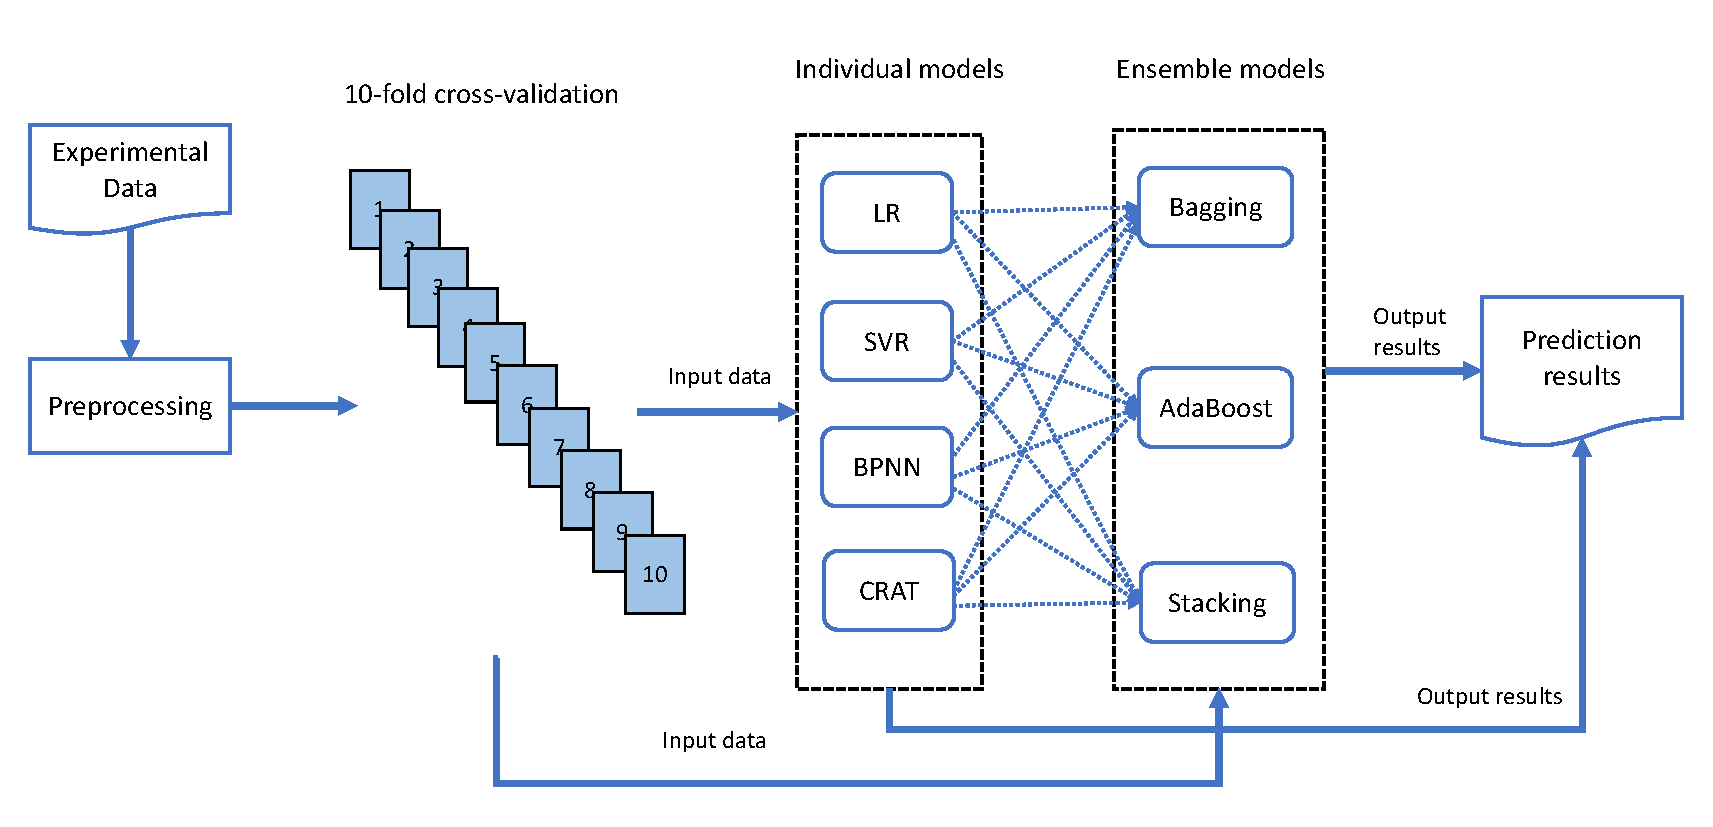
\includegraphics[width=\textwidth]{structure.pdf}
		\end{center}
		\caption{Flow chart of implementing prediction models for self-healing capability of ECC}
		\label{fig:structure}
	\end{figure}
	
	
	This paper is organized as follows.  Section \ref{lab} presents the experimental program detailing the materials used for ECC specimen preparation and the test set-up for crack data measurement. The concepts and formulations of individual and ensemble models used for predicting the self-healing capability of ECC are presented in Section \ref{meth}, whereas the validation and evaluation methods are described in Section \ref{4}. In Section \ref{result}, the computational results are presented and compared, and the model with best prediction performance is identified. Finally, Section \ref{con} draws the major conclusions from this work and suggests some directions for future research.
	
	% 
	%%%%%%%%%%%%%%%%%%%%%%%%%%%%%%%%%%%%%%%%%%
	
	\section{Experimental Program}
	\label{lab}
	
	\subsection{Materials and Mixture Proportion}
	In the experimental part, samples of ECC with different mineral admixtures were prepared. The materials including general purpose cement (GPC), fly ash (FA), silica fume (SF), hydrated lime powder(LP), fine sand, polyvinyl alcohol (PVA) fibers, as well as water and high range water reducing admixture (HRWR) were used. GPC and FA were supplied by Boral in accordance with Australian Standard AS 3972-2010 \cite{noauthor_as_nodate}, while LP was the Adelaide Brighton Hydrated Lime with a specific gravity of 2.2-2.3, and a typical fineness of 0.1\% retained on a 75 $\mu$m sieve and less than 0.05\% on a 250 $\mu$ sieve. The physical and chemical properties of cementitious materials are shown in Table \ref{cm}. Fine sand with an average grain size of 150 $\mu$ and a fineness modulus of 2.01 was used. The PVA fibers were supplied by Domocrete and their mechanical and geometrical properties are described in Table \ref{pva}.

All ECC mixtures were prepared with a constant water to cementitious materials (W/CM) ratio of 0.29 and a constant sand to CM (PC + FA + LP+SF) ratio of 0.36. All  fine aggregates were in saturated surface dried condition prior to mixing. The abbreviations for labelling specimens were adopted in such a way that the letters FA, SF and LP stand for samples with fly ash, silica fume and limestone as binder materials, respectively. The number after the letters shows the percentage of materials into the binder system. For example, the FA70 mixture is related to an ECC sample with binder containing 70\% FA by weight, whereas FA60-SF10 was the mixture with 60\% FA and 10\% SF. A total of nine ECC mixtures were prepared and the details of mix proportion are shown in Table \ref{mx}.

	
		\begin{table}[!h]
		\centering
		\caption{Physical and chemical properties of cementitious materials}
		\begin{tabular}{lcccc}
			\toprule
			\textit{Chemical composition} (\%) &	GPC &	FA&	LP&	SF\\
			\midrule
			Silica (\ce{SiO2})	&19.8 &	65.90 &	1.8&	95.10	\\
			Alumina (\ce{Al2O3})	& 5.3&	24.0&	0.5&	0.21	\\
			Iron oxide (\ce{Fe2O3}) &3.0	&2.87&	0.6	&0.29	\\
			Calcium oxide (\ce{CaO}) &	64.2 &	1.59 &	72.0 &	-	\\
			Magnesia (\ce{MgO})&1.3 &	0.42 &	1.0	 & -	\\
			\ce{R2O}	&0.6 &	1.93 &	- &	- \\
			Sulfur trioxide (\ce{SO3}) &	2.7	& - & - & -	\\
			Titanium oxide (\ce{TiO2})	&0.28 &	0.91 &	-  & -	\\
			Manganic oxide (\ce{Mn2O3}) & 0.22 & - & - & - \\	
			Zirconia (\ce{ZrO2}) + Hafnium (\ce{HfO2}) & -  & - & -	&3.46	\\
			& & & &\\
			Loss on ignition (\%) &	2.8	&1.53&	24.0&	1.4	\\
			Density ($g/cm^3$)	& 3.08 &	2.43 &	2.25 &	2.26	\\
			Specific surface area ($m^2/kg$) &	- &	655	&460 &	$1.5 \times 10^4$	\\
			\bottomrule
		\end{tabular}
		\label{cm}
	\end{table}
	
	\begin{table}[!h]
		\centering
		\caption{Properties of PVA}
		\begin{tabular}{ccccccc}
			\toprule
			Length &Length/&	Young’s modulus &	Elongation &Tensile strength &	Density \\
			(mm)	& diameter ratio & (MPa) & (\%)	 & (MPa) & (g/cm3) \\
			\midrule
			8&	200	&42000&	7&	1600&	1.3
			\\
			\bottomrule
		\end{tabular}
		\label{pva}
	\end{table}
	

	
	
	
	\begin{table}[!tp]
		\centering
		\caption{Mix proportion of all ECC mixtures}
		\begin{tabular}{lccccccccc}
			\toprule
			Mix&	Water/CM	&Sand&	Water&	fibre (V)&	GPC	&Fly ash&	SF&	LP&	HRWR
			\\
			\midrule
			FA70&	0.29&	419.67&	338.07	&26	&349.73&	816.03	&0.00&	-	&5.13
			\\
			FA65-SF5&	0.29&	419.67&	338.07&	26	&349.73	&757.74&	58.29&	-&	5.13
			\\
			FA60-SF10	&0.29&	419.67&	338.07&26&	349.73&	699.45&	116.58	&-&	5.13
			\\
			FA55-SF15&	0.29&	419.67&	338.07&	26&	349.73&	641.16&	174.86	&-&	5.13
			\\
			FA65-LP5&	0.29&	419.67	&338.07&	26	&349.73	&757.74	&-	&58.29&	5.13
			\\
			FA60-LP10&	0.29&	419.67&	338.07&	26&	349.73	&699.45	&-	&116.58	&5.13
			\\
			FA55-LP15&	0.29&	419.67&	338.07&	26&	349.73	&641.16	-&	174.86	&5.13
			\\
			FA55-SF5-LP10&	0.29&	419.67&	338.07	&26&	349.73&	641.16	&58.29	&116.58	&5.13
			\\
			FA55-SF10-LP5	&0.29	&419.67	&338.07	&26	&349.73	&641.16	&116.58	&58.29	&5.13
			\\
			\bottomrule
		\end{tabular}
		\label{mx}
	\end{table}
	

\subsection{Sample preparation and crack measurement}
	\label{experi}
	A planetary-type mixer of 50 L capacity was used to produce ECC specimens. During the mixing process, the solid ingredients including cement, mineral admixtures and sand were initially placed into the mixer and dry mixed for 30 seconds. Then, the water with HRWR was added and the mixture was mixed for 2 minutes. After that, the PVA fibers were slowly added and mixing was continued until uniform distribution of fibers in the mix. After mixing, ECC pastes were cast into standard moulds with dimension of $\O 100mm \times 200mm$. The specimens were demolded 24 hours after casting and stored in a curing room with a temperature of $23 \pm 2^\circ C$ and the relative humidity (RH) of $90 \pm 5\%$ for 28 days for 28 days. To prepare splitting tensile test samples,the cylinder specimens were cut into specimens with a diameter of 100 mm and a thickness of 50 mm using a diamond blade saw.

A newly developed splitting tensile test apparatus was used to generate micro-cracks as shown in Figure \ref{f:cr1} (a). It consisted of a steel frame, top member, bottom member, prestressed loading steel plates (5 mm thick) on both sides with loading nuts and wire springs, as shown in Figure \ref{f:cr1} (b). Both steel plates were connected to the steel frame by nuts and wire springs. The specimen was placed inside the steel frame and then pre-stressed by the steel plates from both sides limiting the propagation and size of crack and preventing excessive crack growth.

Micro-cracks less than 150 $\mu$m were produced by pre-loading the ECC samples up to 70\% of their maximum splitting strength. A digital microscope was used to measure the crack width on the surface of specimens as shown in Figure \ref{f:cr1} (c). After the pre-loading, the cracked specimens were subjected to wet-dry (W/D) cycles to promote self-healing. Each W/D cycle consisted of submersion in water  for 24 hours and drying in laboratory conditions at $23 \pm 2^\circ C$ and a RH of $50 \pm 5\%$ for 24 hours. After 10 W/D cycles, the cracks were measured again by the digital microscope to examine partial or full closure of crack. Figure \ref{f:cr2} illustrated the self-healing of cracks of an ECC specimen before and after the 10 W/D cycles.


	
		\begin{figure}[!h]
		\centering
		\begin{subfigure}{0.31\textwidth}
			\centering
			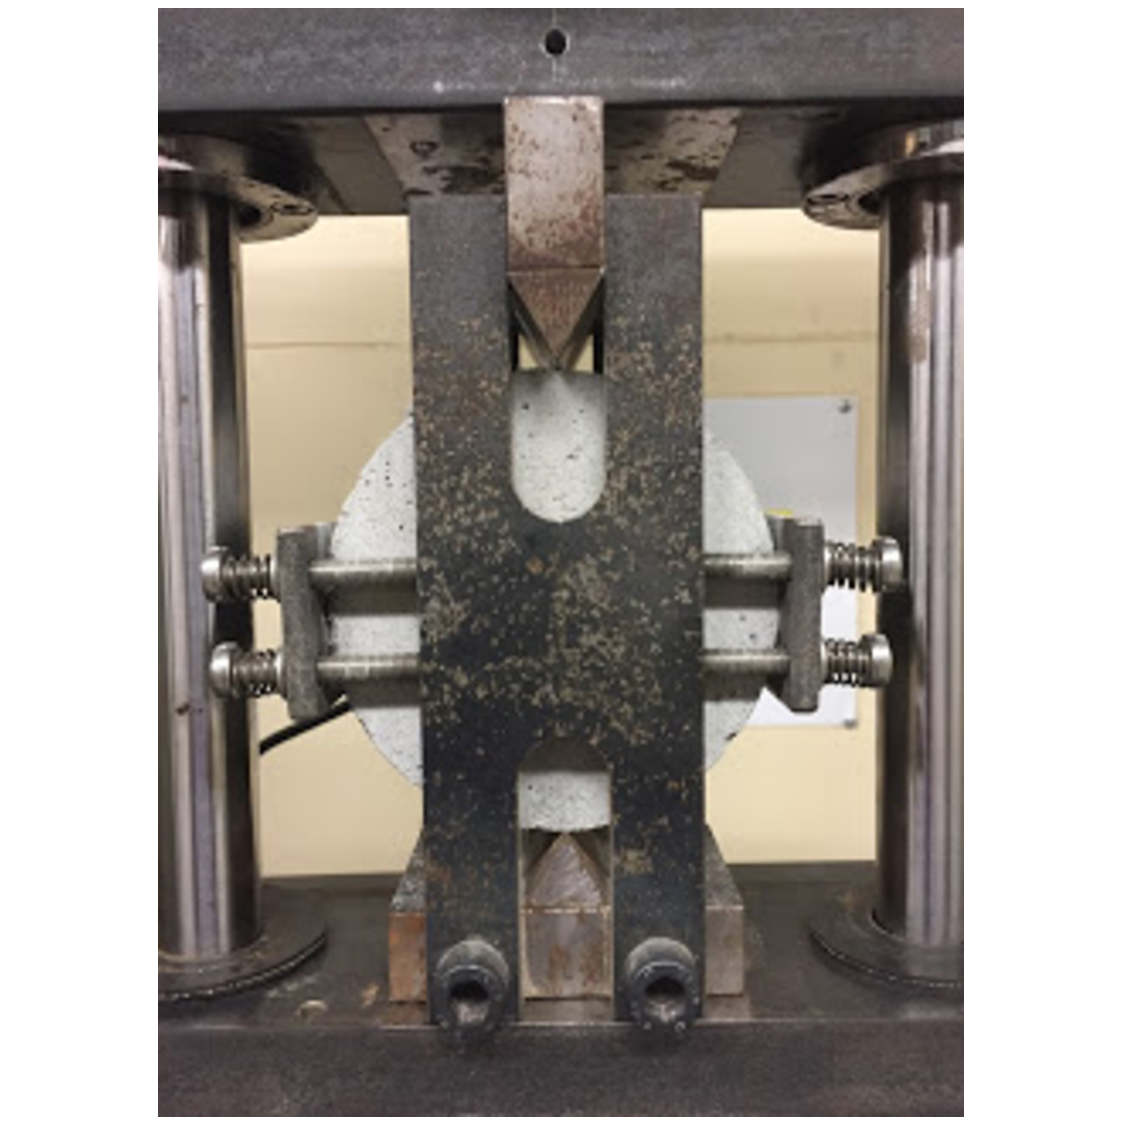
\includegraphics[width = \linewidth]{CR2}
			\caption{Splitting tensile test apparatus}
		\end{subfigure}
	\hspace{-0.1em}
		\begin{subfigure}{0.31\textwidth}
		\centering
		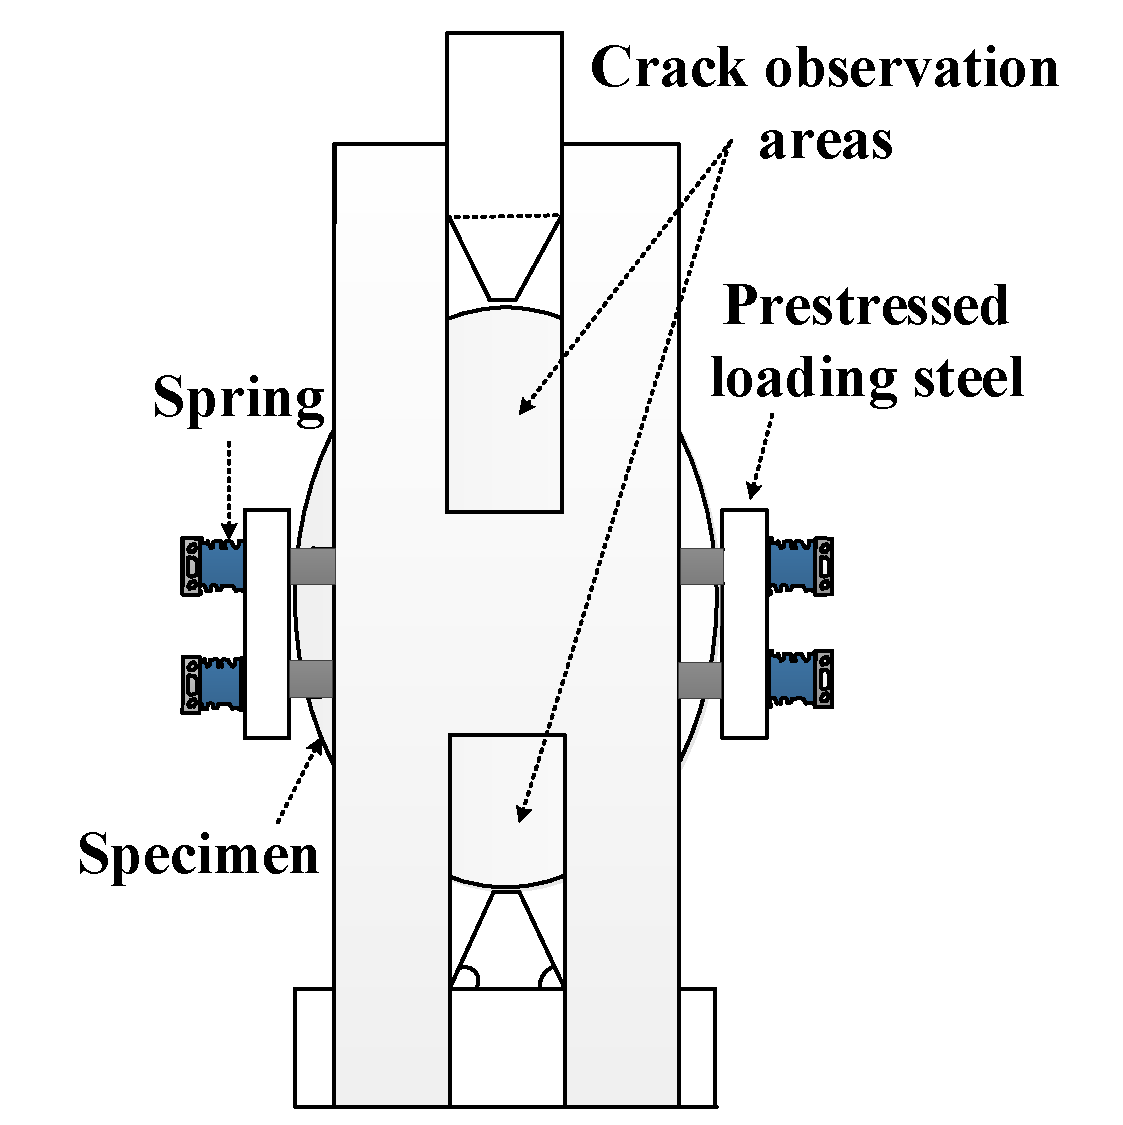
\includegraphics[width = \linewidth]{CR1}
		\caption{Schematic diagram of apparatus}
		\end{subfigure}	
	\hspace{-0.10em}
		\begin{subfigure}{0.31\textwidth}
		\centering
		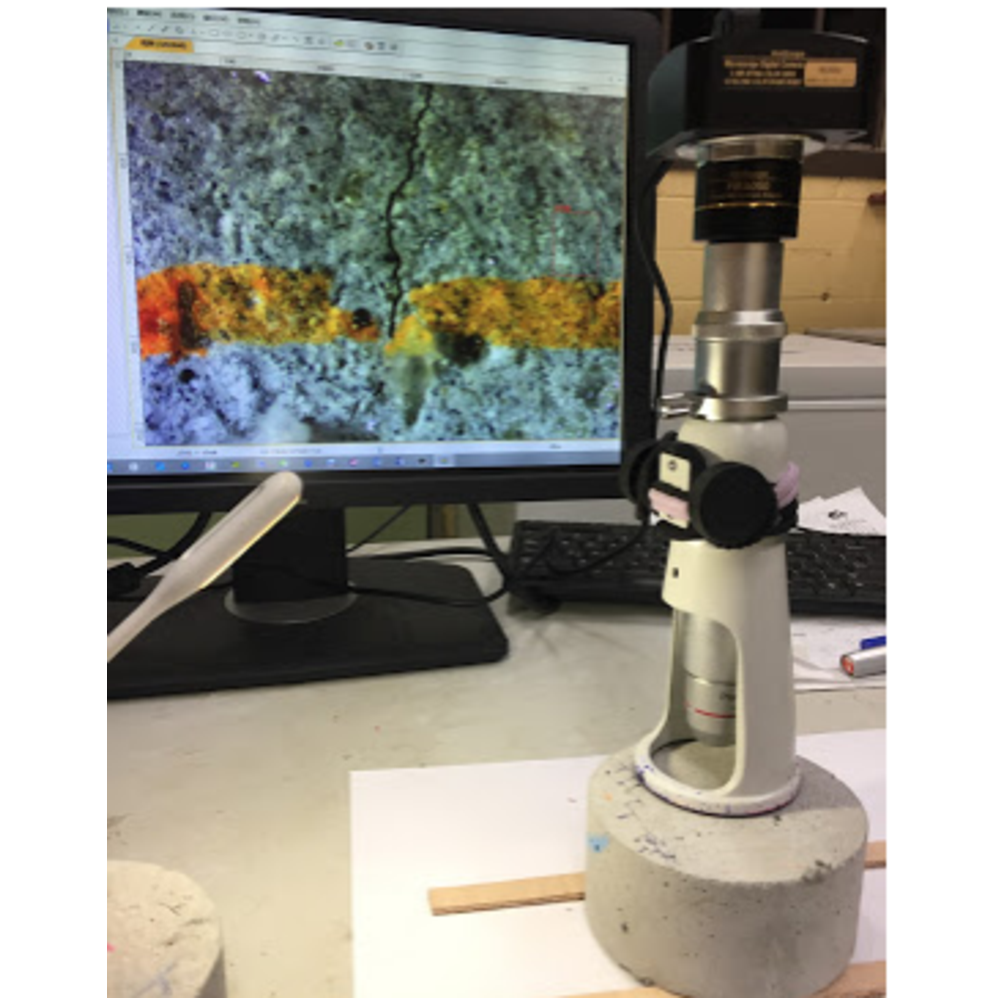
\includegraphics[width = \linewidth]{CR3}
		\caption{Crack width measurement}
		\end{subfigure}
		\caption{Splitting tensile test apparatus and microscope used in experiment for creating and measuring ECC cracks}\label{f:cr1}
	\end{figure} 


	

	
	\begin{figure}[!h]
	\centering
	\begin{subfigure}{0.3\textwidth}
		\centering
		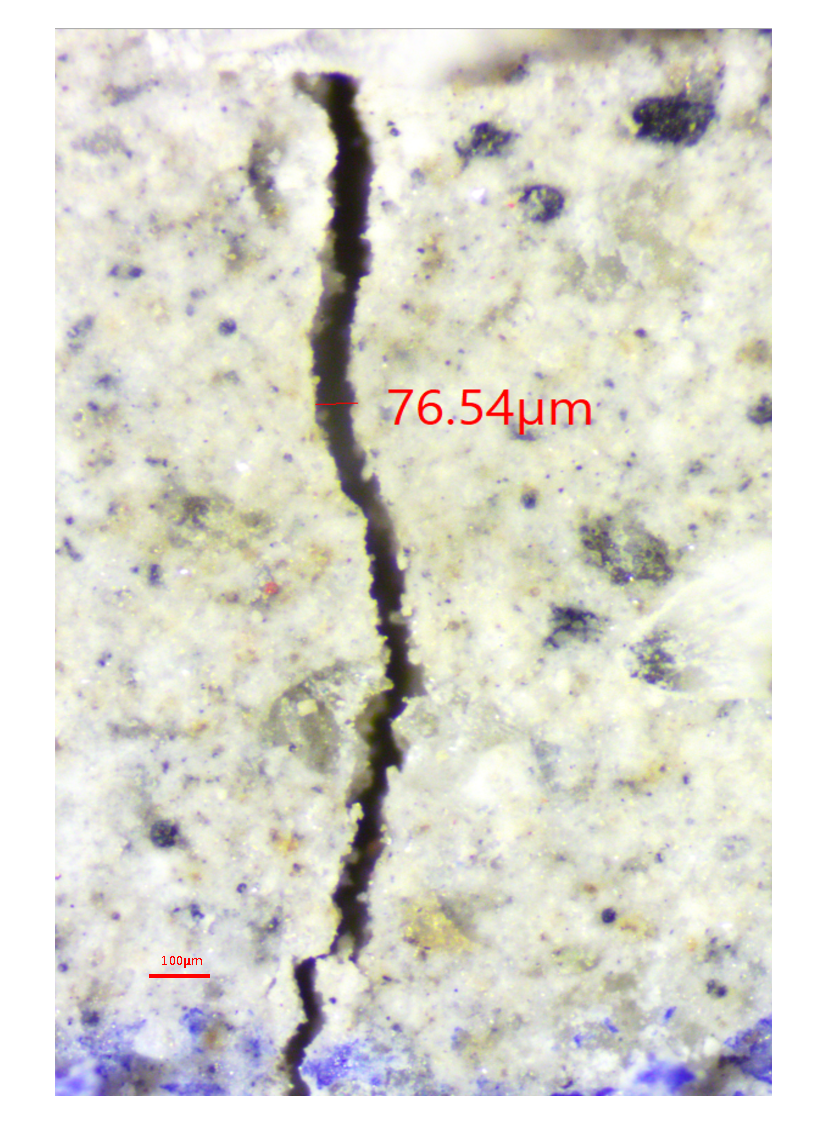
\includegraphics[width = \linewidth]{crack11}
		\caption{S1: crack before self-healing}
	\end{subfigure}
	\hspace{1em}
	\begin{subfigure}{0.3\textwidth}
		\centering
		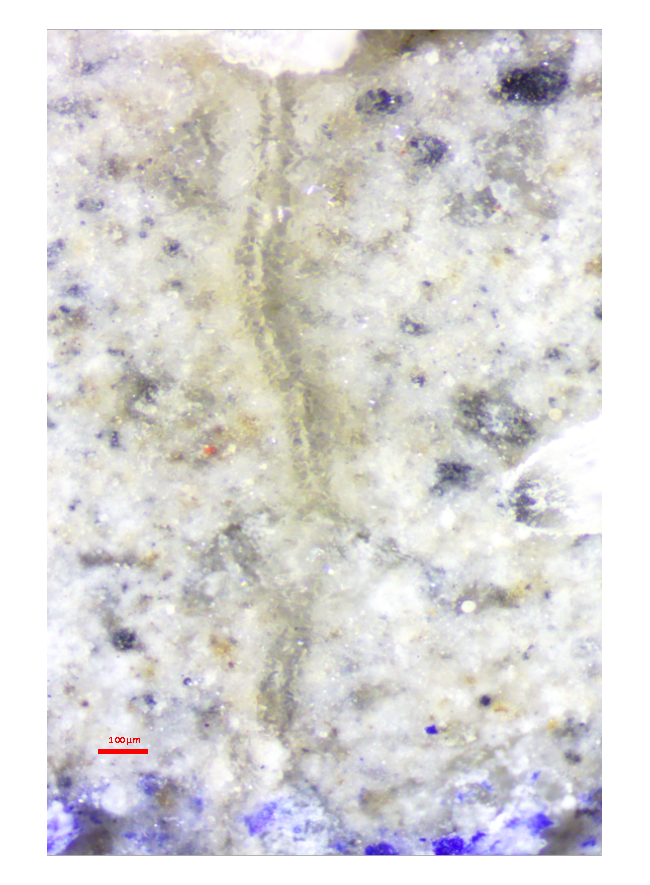
\includegraphics[width = \linewidth]{crack1}
		\caption{S1: crack after self-healing}
	\end{subfigure}	
%		\subfigure[]{%
%			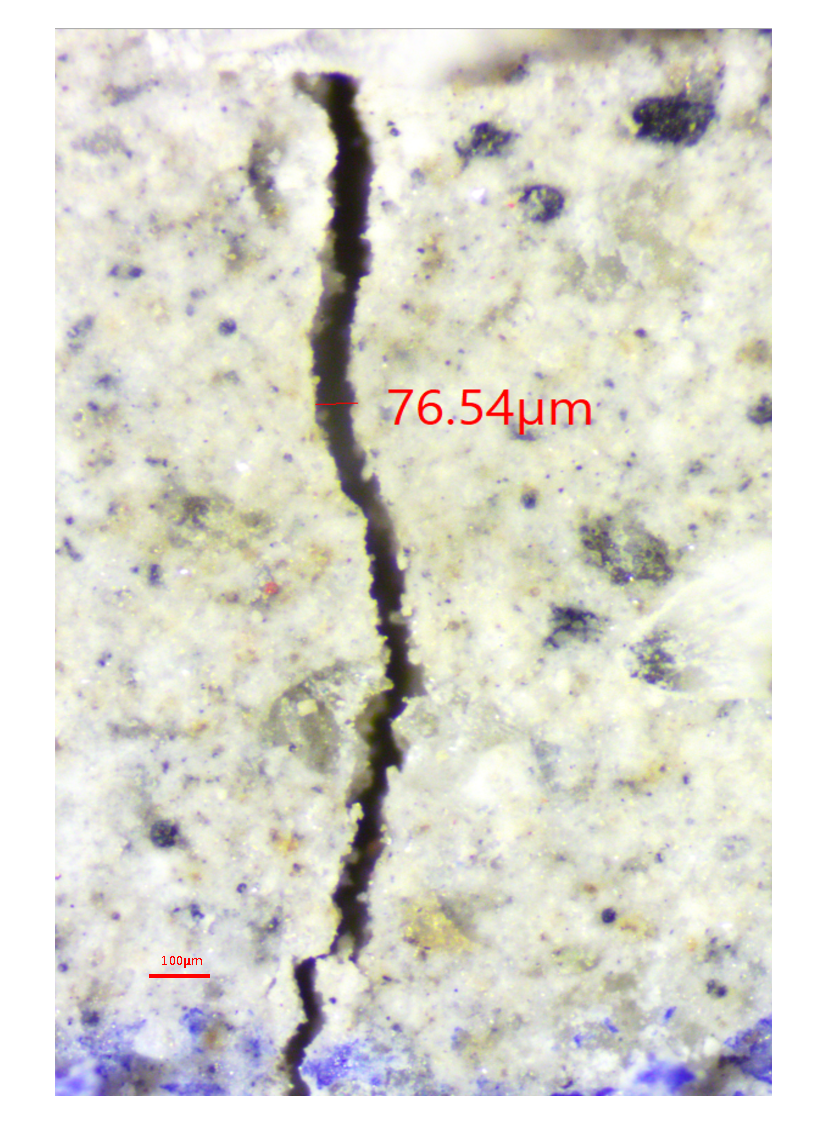
\includegraphics[width=.25\textwidth]{crack11}}\hfill
%		\subfigure[]{%
%			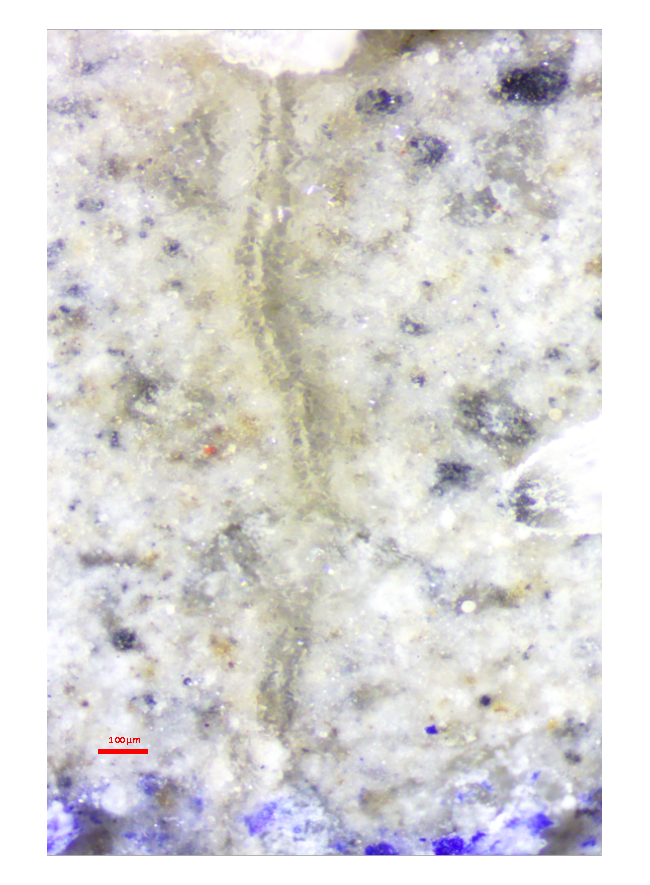
\includegraphics[width=.25\textwidth]{crack1}}\hfill
%		\subfigure[S2: crack before self-healing]{%
%			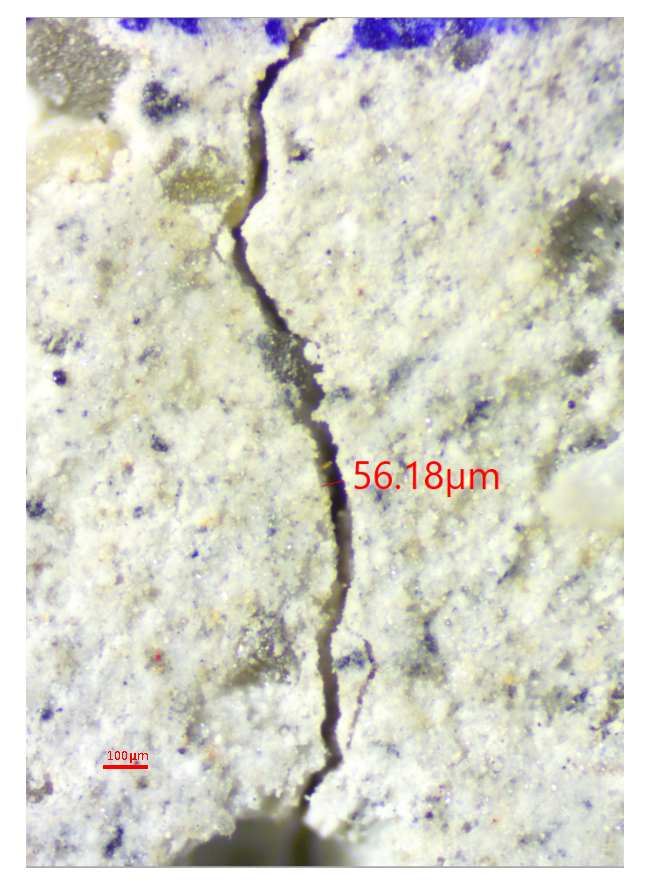
\includegraphics[width=.25\textwidth]{crack2}}\hfill
%		\subfigure[S2: crack after self-healing]{%
%			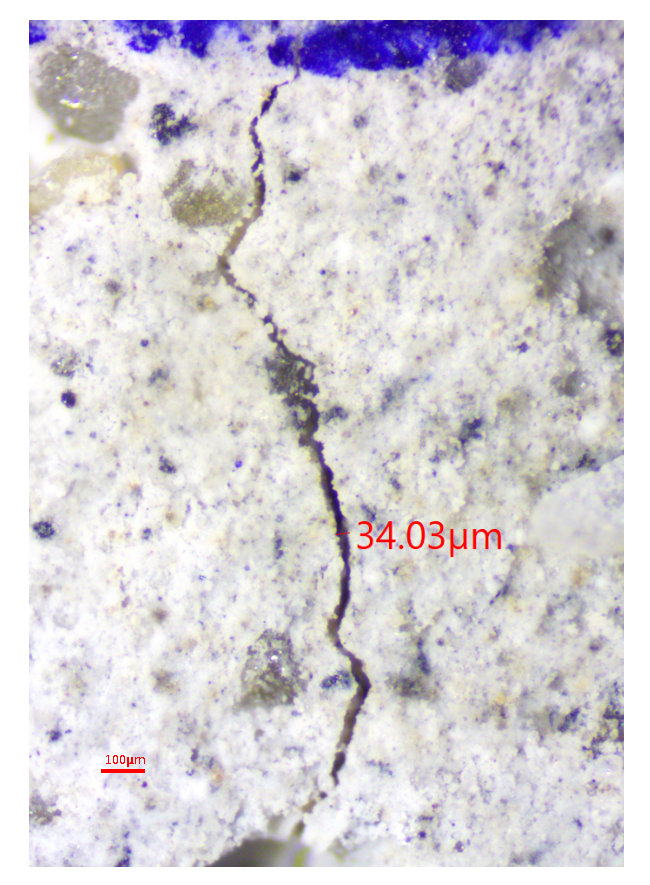
\includegraphics[width=.25\textwidth]{crack22}}\hfill
		\caption{Comparison of crack width changes in two ECC specimens, S1 and S2, before and after self-healing}\label{f:cr2}
	\end{figure}
	
	
%\subsection{The quantitative definitions for self-healing of ECC}
%
%To define the self-healing ability of ECC quantitatively, the crack width before  
%		
		
	\subsection{Data Collection}
	\label{dc}
	
	\begin{figure}[!h]
		\centering
		\includegraphics[width=.75\textwidth]{measurement}
		\caption{Schematic diagram of measuring observation areas on the surface of ECC mixture specimen}
		\label{ma}
	\end{figure}
	
	
	Experimental data for prediction were gathered with four features, including crack width before self-healing (representing the influencing factor of self-healing), and the mineral contents of  FA, SF, and LP. It is noteworthy that the factors such as GPC, sand, W/CM, and healing time were kept  constant and hence, they were excluded in the prediction modeling. For each ECC mixture, there were 6 identical test specimens. After pre-loading, the crack widths of the specimens were measured using the digital microscope before and after the self-healing. Four horizontal lines were drawn on the surface of each specimen along the direction of vertical force, which divided the specimen into five observation areas. The schematic diagram of the measurement is shown in Figure \ref{ma}. In each observation area, only one crack data was recorded if the crack width showed little or no change along the vertical force, otherwise, multiple crack data would be collected. Totally, 617 crack data samples were collected from nine mixtures to construct the ML training-testing dataset \cite{chen2021selfhealing}. Table \ref{min} shows the number of collected samples and range of crack width before and after self-healing in each mixture. 
	

	\begin{table}[!h]
		\centering
		\caption{Number of crack samples and range of crack width before and after self-healing collected from the ECC mixes}
		\label{min}
		\begin{tabular}{p{1.02in}p{1.2in}cccc}
			\toprule
			&		&	\multicolumn{2}{p{1.9in}}{Crack width before self-healing}	&	\multicolumn{2}{p{1.8in}}{Crack width after self-healing}	\\ \cmidrule(r){3-6}
			Mix	&	Number of crack samples	&	Min	($\mu m$) &	Max ($\mu m$)	&	Min ($\mu m$)	&	Max ($\mu m$)	\\
			\midrule
			FA70	&	87	&	3.28	&	134.69	&	0	&	121.37	\\
			FA65-SF5	&	77	&	4.37	&	135.47	&	0	&	124.01	\\
			FA60-SF10	&	88	&	5.18	&	121.78	&	0	&	113.11	\\
			FA55-SF15	&	88	&	3.45	&	115.8	&	0	&	109.53	\\
			FA65-LP5	&	112	&	7.65	&	119.45	&	0	&	105.65	\\
			FA60-LP10	&	37	&	5.62	&	126.82	&	0	&	110.97	\\
			FA55-LP15	&	61	&	6.42	&	132.65	&	0	&	115.95	\\
			FA55-SF5-LP10	&	34	&	8.74	&	123.09	&	0	&	110.78	\\
			FA55-SF10-LP5	&	33	&	4.64	&	131.57	&	0	&	119.79	\\
			%Total	&	617	&	-	&	-	&	-	&	-	\\
			\bottomrule
		\end{tabular}
	\end{table}
	

	
	\subsection{Preprocessing of Data}
	
	Since the input and output data of different features vary in range and units, the features with bigger number would steer the model performance. As shown in Table \ref{mx}, the range of FA varies from 641.16 to 816.03 kg, but the range of SF varies from 0 to 174.86 kg. From Table \ref{min}, the range of crack width varies from 0 to 135.47 $\mu$m. To eliminate this potential bias, the experimental data was preprocessed through the min-max normalization to scale the range of all features into[0,1] with the following equation: 
	
	\begin{equation}
	x' = \frac{x - x_{min}}{x_{max} - x_{min}}
	\end{equation}
	
	
	Where $x'$ was the scaled value of the variable $x$, $x_{max}, x_{min}$ were the maximum and minimum values of variable $x$ respectively.
	

	
	%%%%%%%%%%%%%%%%%%%%%%%%%%%%%%%%%%%%%%%%%%
	
	
	\section{Proposed Machine Learning Models }
	\label{meth}
	

	
To predict the self-healing capability of ECC, four individual ML models including LR, SVR, BPNN and CART, and three ensemble methods including bagging, AdaBoost and stacking were proposed. Ensemble models were constructed using individual models as the base estimators. To establish a baseline for comparison, the modeling parameters were set to be the same in both individual models and ensemble models. The reason for choosing these techniques was due to their popularity and some of them were even recognized as the top data mining algorithms in related fields of concrete \cite{chou2014machine}. The proposed individual and ensemble techniques are described in the following subsections.
	
	
	\subsection{Linear Regression}
	
	LR attempts to determine the relationship between a dependent variable (response variable) and one or more independent variables (explanatory variables) by fitting a linear regression equation \cite{neter1996applied}. Given our dataset $T = \{ (x_i,y_i), i = 1,2,...,n\}$, where $n = 617$ was the size of sample dataset. $x_i \in R^n$ was independent variables representing a sample of selected features from FA, SF, LP and crack width before self-healing, $R^n$ was $n$-dimensional space, $y_i \in R^1$ was the target output (crack width after self-healing) that corresponded to $x_i$. Let $d = 4$ denote the number of an independent variable  of a random vector $x = \{ x_1;x_2;...;x_d \}$, and $y$ was the corresponding output ( dependent variable). The general formula of LR for predicting self-healing capability of ECC can be expressed as follows:
	
	\begin{eqnarray}
	y = w_1 x_1 + w_2 x_2 + ......+ w_d x_d +b                                                      
	\end{eqnarray}
	where $w_i, (i = 1,2,...,d)$ was denoted as the regression coefficient, $b$ was an error term. The prediction performance of LR was used as a benchmark to compare the performance of other individual and ensemble models in this study. 
	
	\subsection{Support Vector Regression}
	
	The support vector machine (SVM) is a supervised machine learning method first introduced by Vapnik \cite{cortes1995support,vapnik1999overview} based on statistical learning theory \cite{juncai2015prediction}. Since then, it has gained popularity due to attractive features, and promising empirical performance. SVM includes two main categories: support vector classification (SVC) and SVR. For classification purposes, SVMs often used a \textit{kernel} function to map the input data as vectors to a high-dimensional feature space so that an optimal separating hyperplane can be constructed \cite{suykens1999least}. 
	
	For regression purposes, the basic idea is to provide a nonlinear function by mapping input data into a high-dimensional feature space, where a special type of hyperplane is constructed. After that, a regression model is established in the hyperplane \cite{li2007consensus}. 
	
	Given our dataset $T = \{ (x_i,y_i), i = 1,2,...,n\}$, where $n = 617$ was the size of sample dataset, $x_i \in R^n$ was the input vector representing selected features of a sample, including FA, SF, LP and crack width before self-healing, $R^n$ was the $n$-dimensional vector space, $y_i \in R^1$ was the target output indicating crack width after self-healing that corresponded to $x_i$. The SVR aimed to seek an optimum regression function $f(x)$ with minimal empirical risk, which can be expressed as follow:
	
	\begin{eqnarray}
	f(x) = \langle w,x \rangle + b \quad \text{with} \quad w \in T, b \in R                                                              
	\end{eqnarray}
	where $\langle \cdot, \cdot \rangle$ was denoted as the dot product in $T$, $w$ and $b$ were the weight vector and bias value which are estimated by minimizing the empirical risk, that was, the distance between the predicted crack width and the target crack width after self-healing.  
	
	SVR adopts an $\epsilon$-insensitive loss function penalizing predictions that has a distance between the predicted crack width and the target crack width when the self-healing is greater than $\epsilon$. Therefore, the problem of finding $w$ and $b$ to reduce the empirical risk with respect to an $\epsilon$-insensitive loss function is equivalent to the convex optimization problem that minimizes the margin ($w$) with the full prediction error within the range of $\epsilon$. Then this problem can be expressed as: 
	%:
	\begin{eqnarray} \label{svr2}
	\begin{aligned}
	\text{minimize} \quad& \frac{1}{2} ||w||^2 \\
	\text{subject to} \quad & 
	\left  \{ 
	\begin{array}{l}
	y_i -\langle w,x_i \rangle -b \le \epsilon \\
	\langle w,x_i \rangle +b -y_i \le \epsilon
	\end{array}
	\right.
	\end{aligned}                                                            
	\end{eqnarray}
	By introducing slack variables $\xi, \xi_i^*$ to allow some errors to cope with infeasible solution of the optimization problem, the formulation can be generated as \cite{vapnik1999overview}: 
	
	\begin{eqnarray}
	\begin{aligned}
	\text{minimize} \quad &  \frac{1}{2} ||w||^2 + C \sum_{i=1}^{n}(\xi + \xi_i^*) \\
	\text{subject to} \quad& 
	\left \{
	\begin{array}{l}
	y_i - \langle w, x_i \rangle -b \le \epsilon + \xi_i \\
	\langle w, x_i \rangle + b - y_i \le  \epsilon + \xi_i^* \\
	\xi_i, \xi_i^* \ge 0 
	\end{array}
	\right.
	\end{aligned}                                                              
	\end{eqnarray}
	
	The constant $C$ was the penalty value imposed on predictions that lied outside the $\epsilon$ margin. Lagrange multipliers are included to solve this problem. By constructing the objective function and all constraints, a dual set of variables are introduced as follows: \cite{yuvaraj2013support}:
	\begin{eqnarray}
	\begin{aligned}
	L_P  = & \frac{1}{2} ||w||^2 +C\sum_{i=1}^{n} (\xi_i + \xi_i^*) - \sum_{i=1}^{n} (\eta_i \xi_i + \eta_i^* \xi_i^*) \\
	& -\sum_{i=1}^{n} \alpha_i (\epsilon + \xi_i - y_i + \langle w, x_i \rangle + b) \\
	& - \sum_{i=1}^{n} \alpha_i^* (\epsilon + \xi_i^* +y_i - \langle w, x_i \rangle -b )
	& \\
	s.t. \quad & \alpha_i, \alpha_i^*, \eta_i, \eta_i^* \ge 0 
	\end{aligned}.                                                               
	\end{eqnarray}
	
	Where $L_P$ was the Lagrangian and $ \alpha_i, \alpha_i^*, \eta_i, \eta_i^* $ were Lagrange multipliers.
	
	The optimality can be achieved by the partial derivatives of $L_P$ with respect to the primal variables following the saddle point condition. Then the function of SVR is obtained as:
	\begin{eqnarray}\label{svr3}
	f(x) = \sum_{i=1}^{n} (\alpha_i - \alpha_i^*)\langle x_i , x \rangle +b                                                             
	\end{eqnarray}
	
	As for the nonlinear regression, the input data have to be mapped into a high-dimensional feature space, in which the dot product can be replaced by a kernel function $k(x_i, x_j) = \phi(x_i)^T\phi(x_j)$, and the function \eqref{svr3} can be written as:
	\begin{eqnarray}
	f(x) = \sum_{i=1}^{n}(\alpha_i - \alpha_i^*)k(x_i , x) +b                                                          
	\end{eqnarray}
	
	Different SVM algorithms use differing kinds of kernel functions such as linear, polynomial, radial basis function and sigmoid kernel. In this work, the Gaussian radial basis function (RBF) was chosen, which was defined as \cite{smola2004tutorial}:

	\begin{eqnarray}
	k(x_i, x_j) = exp ({- \frac{||x_i -x_j ||^2}{2 \sigma^2} })                                                           
	\end{eqnarray}
	
	
	\subsection{Artificial Neural Network}
	Artificial neural network (ANN), also called neural network,is originated from simulating biological neural networks. Generally, it consists of many neurons in layers including one input layer, one or several hidden layers and an output layer \cite{mukherjee1997artificial}. The neurons are fully interconnected between the neighboring layers by weight, and typically no inter-connections between neurons within the same layer \cite{naderpour2018compressive}. 
	
	There are many possible network structures available, BPNN was utilized in this study because of back-propagation (BP) algorithms is the most widely used and effective learning algorithm for training an ANN. A preliminary architecture of the BPNN was determined to be 4 - $n$ - 1, where 4 input neurons represented the input features standing for FA, LP, SF and crack width before self-healing, $n = 5$ indicated the number of neurons in the hidden layer, and 1 target neuron in the output layer for the predicted crack width after self-healing. This is a three-layer network with one hidden layer capable to approximate most continuous functions, of which the complex nonlinear relationship could be approximated in accuracy \cite{yan2017evaluation}. The architecture of the BPNN model for predicting self-healing is demonstrated in Figure \ref{fig:BPNN}. %Details of input parameters see in Section \ref{experi} and \ref{dc}.
	
	\begin{figure}[!]
		\begin{center}
			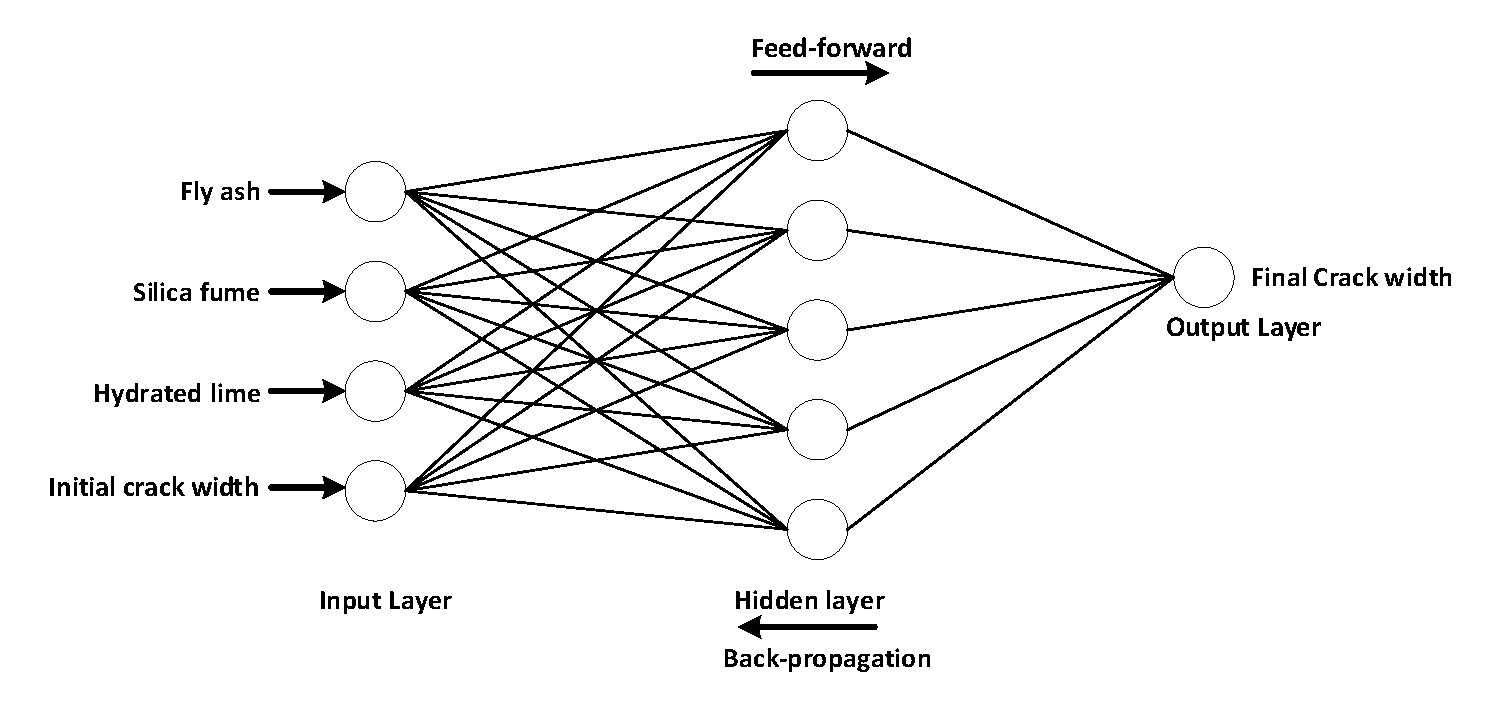
\includegraphics[width=\textwidth]{BPNN.pdf}
		\end{center}
		\caption{Schematic diagram of BPNN model for predicting self-healing capability of ECC}
		\label{fig:BPNN}
	\end{figure}
	
	Given a set of inputs $ \{ x_1, x_2,x_3,..., x_n\}$, while information was passed through the input layer to the hidden layer, each neuron in the input layer was multiplied by respective weights added by a bias and are summed together. After that, an activation function $f$ was applied to form the output $z$. This can be expressed in the following equation \cite{alshihri2009neural}:
	
	\begin{equation}
	z = f(\sum_{i=1}^{n} w_{ij}x_i + b_j)
	\end{equation}
	
	where $w_{ij}$ was the connection weights between the $i$th neuron of input and the $j$th neuron in the hidden layer, and $b_j$ was the bias of the $j$th neuron. The sigmoid function was applied as the activation function between the input, hidden, and output neurons to form the output. 
	
	\begin{equation}
	f(x) = \frac{1}{1+e^{-x}}
	\end{equation}
	
	The goal of training a neural network is to determine the values of the connection weights and the biases of the neurons. The back propagation indicates an iterated method to adjust the weights from output layer to input layer. At first, the outputs were calculated feed-forward from the input layer via the hidden layer to the output layer. Then an error was generated by comparing the output with the target output. After that, the error was back propagated to the hidden layer and input layer. By adjusting the connection weights and biases, the error was further reduced. The process was repeated until the error was minimised or reaching the termination to avoid over-fitting. 
	
	\subsection{Classification and Regression Tree}
		The CART \cite{breiman2017classification}  is a tree decision algorithm that splits data into mutually exclusive subgroups based on recursive binary partitioning procedure. It develops the relationship between the target variables (the crack width after self-healing of ECC) and the independent variables (the input features of FA, SF, LP and crack width before self-healing of ECC) to create decision rules to form subgroups as branches and leaves as shown in Figure \ref{fig:CART}. The process of CART starts from the root node which contains the entire data set to construct two sub-nodes representing two categories. Then this recursion process is applied to each sub-node until all divided sub-nodes are leaf nodes. The CART tree can be either a classification tree \cite{dan1995cart} or regression tree \cite{put2003classification} depending on the type of target and independent variables which may be categorical or numerical. 
	

	
	\begin{figure}[!htb]
		\begin{center}
			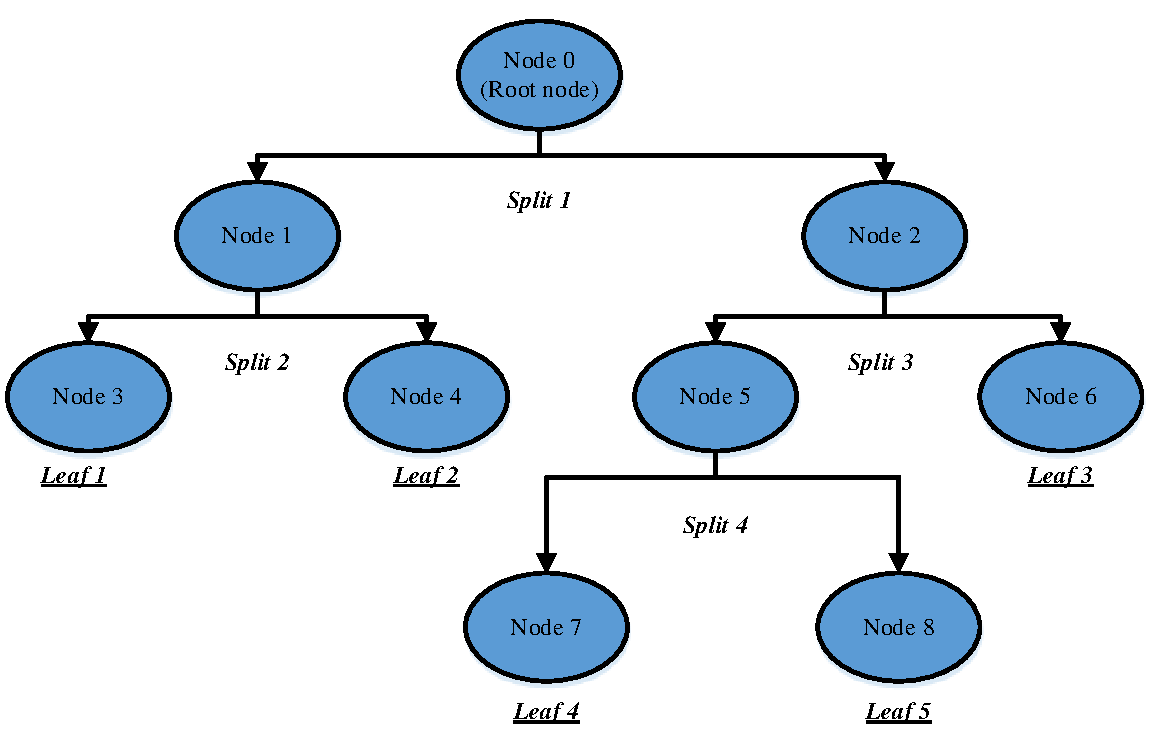
\includegraphics[width=0.75\textwidth]{CART}
		\end{center}
		\caption{Structure of a classification and regression tree \cite{put2003classification}}
		\label{fig:CART}
	\end{figure}
	
	
The key idea of constructing a CRAT tree is achieved by selecting a variable at each node that best splits the empirical data. To locate splits, $Gini$ index was used to measure the impurity of the two child nodes containing subsets of data that were as homogeneous as possible with respect to the target variable.

	Given a dataset had $K$ classes and the probability of a record in the dateset which belongs to class $i$ is $p_i$, $i \in \{1,2,3,...,K\}$, the $Gini$ impurity can be expressed as:
	
	\begin{equation}
	G(p) = \sum_{i=1}^{K}p_i(1-p_i) = 1- \sum_{i=1}^{K}p_i^2
	\end{equation}
	
	
	\subsection{Ensemble Methods}
	In contrast to many ML approaches such as SVM and CART (which develop a single learner from training data), ensemble methods train multiple base learners and combine them \cite{chou2014machine} to improve generalizability over a single estimator. Therefore, weak learners (base learners) can be boosted to become strong learner \cite{frosyniotis2003divide} in an ensemble method. The base learners in an ensemble were developed from an individual learning algorithm such as decision tree, SVM, or other kinds of learning algorithms. Breiman \cite{dietterich2000ensemble} showed that ensemble methods are usually more accurate than individual learning methods.
	
	The input features of FA, SF, LP, and crack width before self-healing of ECC were considered as the $d$-dimensional predictor variable $X$, whereas, the crack widths after self-healing of ECC were the one dimensional output $Y$.  Each estimator used an individual algorithm to provide one estimated function $g(\cdot)$. The output presented by ensemble-based function $g_{en}(\cdot)$ was obtained by a linear combination of individual functions. This ensemble approach can be expressed mathematically as:
	
	\begin{equation}
	g_{en}(\cdot) = \sum_{j=1}^{N}c_j *g(\cdot)
	\end{equation}
	
	Where $c_j$ expressed as the combination coefficients, dependent on the used ensemble models.  
	
	\subsubsection{Bagging}
	Bagging method (bootstrap aggregating) can generate multiple versions of a predictor to obtain an aggregated predictor \cite{breiman1996bagging}. It generates multiple models independently on different versions of dataset via random bootstrapping of the original training set. In other words, several training examples could repeatedly appear in different bootstrap replicates. Then the individual predictions are aggregated through a combination method (either voting or averaging) to form the final prediction. Bagging method can be used to reduce the variance of a base estimator (e.g. a regression tree), by introducing randomization into its construction procedure and making an ensemble out of it.
This study used four individual models to build bagging ensemble models including a LR bagging ensemble model (abbreviated as Bag$\_$LR), a SVR bagging ensemble model (abbreviated as Bag$\_$SVR), a BPNN bagging ensemble model (abbreviated as Bag$\_$BPNN), and a CRAT bagging ensemble model (abbreviated as Bag$\_$CRAT).


	% In many cases, bagging methods constitute a very simple way to improve with respect to a single model, without making it necessary to adapt the underlying base algorithm.
	
	\subsubsection{AdaBoost}

	
	Similar to bagging, AdaBoost method \cite{freund1996experiments} manipulates the training examples to generate multiple predictions to form the final prediction. The main difference with bagging is that AdaBoost applies a weight to each of the training examples. In each iteration, the weights are individually updated to minimize the weighted error on the training set. For example, weights on those training examples incorrectly predicted in previous iteration increase, whereas the weights of the correctly predicted training examples decrease. Therefore, AdaBoost tends to construct progressively more difficult learning problems in subsequent iterations. Once the training process has finished, the predictions are combined through a weighted majority vote (or sum) to produce the final prediction. So, the final classifier usually can achieve a high degree of accuracy in the test set.
	
By combining four individual models as base estimators in AdaBoost, this study obtained four AdaBoost ensemble models. They are a LR AdaBoost ensemble model (abbreviated as Ada$\_$LR), a SVR AdaBoost ensemble model (abbreviated as Ada$\_$SVR), a BPNN AdaBoost ensemble model (abbreviated as Ada$\_$BPNN), and a CRAT AdaBoost ensemble model (abbreviated as Ada$\_$CRAT). 

	
	\subsubsection{Stacking}

	
	Stacking regression combines multiple regression models via a meta-regressor, using out-of-fold prediction concept \cite{raschkas_2018_mlxtend}. The stacking method used in this work splits the data set into k folds, in which the k-1 folds are used to train the first level regressors in k successive rounds. In each round, the first level regressors are used to predict based on the remaining 1 subset. After that, the prediction results are used and stacked as input data to the second level regressors to form a final set of predictions \cite{sill2009feature}. The schematic diagram of stacking model is shown in Figure \ref{fig:Stack}.  In this study, one stacking based ensemble model (abbreviated as Stack$\_$LR) was proposed based on two levels scheme. SVR, BPNN and CRAT were used as regression models in the first level to get the prediction results, and LR was used as meta-regressor in the second level to combine and generate the final prediction results.
	
	\begin{figure}[!h]	
		\begin{center}
			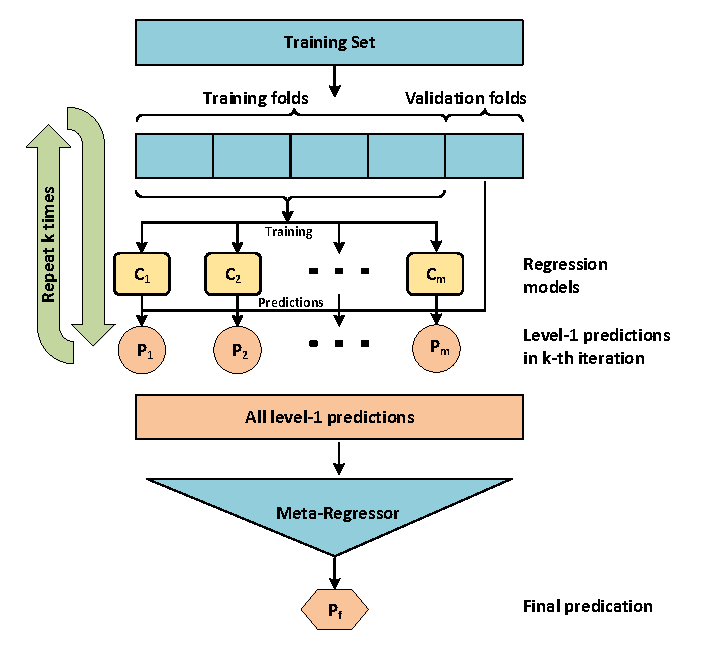
\includegraphics[width=0.75\textwidth]{SP}
		\end{center}
		\caption{Schematic diagram of Stacking model \cite{sill2009feature}}
		\label{fig:Stack}
	\end{figure}
	
	
	
	%%%%%%%%%%%%%%%%%%%%%%%%%%%%%%%%%%%%%%%%%%
	
	
	%%%%%%%%%%%%%%%%%%%%%%%%%%%%%%%%%%%%%%%%%%
	\section{Validation and Evaluation}
	\label{4}
	
	
	
	\subsection{Cross-validation Method}
	\label{cross}
	Generally, dataset is split to generate a training subset and a validation subset keeping the properties of the original dataset as much as possible to avoid misleading estimates. To minimize bias of random data splitting, the K-fold cross-validation is commonly used as it can yield optimal computational time and reliable variance \cite{chou2014machine,kohavi1995study}. In this study, a ten-fold cross-validation approach was applied to assess model performance as shown in Figure \ref{fig:TFC}. The dataset was split randomly into 10 equal-size subsets with a similar distribution. In each validation process, nine of the subsets were used for training and the rest for testing. The process was repeated 10 times \cite{dor2007achieving}. The average accuracy after 10 times validation was reported as the model accuracy.
	
	
	\begin{figure}[!h]
		\begin{center}
			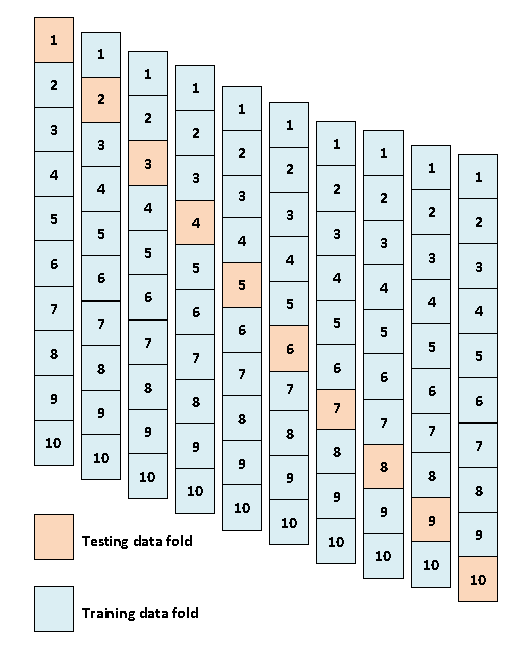
\includegraphics[width=0.65\textwidth,height=0.65\textwidth]{TC}
		\end{center}
		\caption{Ten-fold cross-validation approach}
		\label{fig:TFC}
	\end{figure}
	
	\subsection{Performance Evaluation}
	To show and validate the accuracy of the proposed ML models, three statistical indices namely mean absolute Error (MAE), root mean square error (RMSE), and the coefficient of determination $R^2$ were used and expressed in equations (\ref{fm1}), (\ref{fm2}), and (\ref{fm3}), respectively. The average deviation of the performance of an individual model or an ensemble model from a benchmark model in terms of  three statistical measures (MAE, RMSE and  $R^2$) was calculated using equation (\ref{CP}).
	
	\begin{itemize}
		\item Mean absolute error (MAE). 
		\begin{eqnarray}
		\label{fm1}
		MAE = \frac{1}{n}\sum_{i=1}^{n}{|y_i - y_i^{'}|}                                                       
		\end{eqnarray}
		\item Root mean square error (RMSE)
		\begin{eqnarray}
		\label{fm2}
		RMSE = \sqrt{\frac{1}{n}\sum_{i=1}^{n}({{ y_i  - y_i^{'}}} )^2}                                                         
		\end{eqnarray}
		\item Coefficient of determination ($R^2$)
		\begin{eqnarray}
		\label{fm3}
		R^2 = 1 - \frac{\sum_{i=1}^{n}(y_i - y_i^{'})^2}{ \sum_{i=1}^{n} (y_i -\overline{y})^2  }                                             
		\end{eqnarray}
		\item Deviation ($Dev$)
		\begin{equation}
		\label{CP}
		Dev(\%) = \frac{P_i - P_{j}}{ P_{j}} * 100
		\end{equation}
	\end{itemize} 
	
	Where $y_i$ was the target output, $y_i^{'}$ was the predicted output, $n$ was the number of samples, $\overline{y}$ was the mean of the target output. $Dev$ indicated the statistical performance improvement compared with a benchmark model, $P_i$ was the statistical performance (MAE, RMSE or  $R^2$) of an individual or ensemble method, and $P_j$ was the corresponding performance of a benchmark model, LR or an individual method used in the ensemble method as the base learner.
	
	MAE statistics is a measure of errors between the predicted values (the estimated value of crack width of ECC after self-healing) with the target  values (the observed value of crack width of ECC after self-healing in empirical data). RMSE statistics computes the square root of the average residual error between the predicted values and the target values. A lower value of MAE or RMSE indicates a better prediction performance of the model. $R^2$ measures the strength of association between the predicted values and the target values, based on the proportion of total variation of outcomes. A greater value close to 1 represents a better prediction performance that commendably replicates the observed crack width of ECC after self-healing.  Deviation statistics indicates the improvement of the prediction performance of an individual or an ensemble model from a benchmark model that can be the LR model or the individual model used as base learners in the corresponding ensemble model. 
	
	
	
	%\begin{figure}[!h]
	%	\centering
	%	\includegraphics[width=0.9\textwidth]{01R2.png}
	%	\caption{Average $R^2$ results of all machine learning models on self-healing of ECC}
	%	\label{su}
	%\end{figure}
	
	%%%%%%%%%%%%%%%%%%%%%%%%%%%%%%%%%%%%%%%%%%
	\section{Results and Discussion}
	\label{result}

	In this section, the prediction performance of individual and ensemble methods are examined by MAE, RMSE and $R^2$ according to ten-fold cross-validation. The abbreviation for labelling models were adopted in a such a way that the letters Bag, Ada and Stack stand for the ensemble methods of Bagging, AdaBoost and Stacking, respectively. The letters LR, SVR, BPNN and CRAT stand for the base estimators. However, the Stack\_LR model refers to combining the base methods including SVR, BPNN, and CRAT in the first level and using LR as a meta-regressor in the second level.
	
% 	Where we use the abbreviations for ease of presentation, in which Bag\_LR, Bag\_SVR, Bag\_BPNN and Bag\_CRAT express generating bagging ensemble method by using LR, SVR, BPNN and CRAT as base estimators, respectively. Ada\_LR, Ada\_SVR, Ada\_BPNN and Ada\_CRAT present generating AdaBoost ensemble method by manipulating LR, SVR, BPNN and CRAT as base estimators, respectively. Stack\_LR indicates developing stacking ensemble method based on individual methods (including SVR, BPNN, and CRAT) as learning base with using LR as a meta-regressor. 
	
	\subsection{Prediction performance assessment}
	
	Table \ref{per} shows the average performance of individual and ensemble models. The ten-fold cross-validation results (MAE, RMSE, and $R^2$) for both individual and ensemble models and their deviation with respect to the results of LR model. 
		\begin{table}[!h]
		\small
		\centering
		\caption{Average performances of machine learning models for self-healing prediction of ECC}
		\begin{tabular*}{0.75\textwidth}{ll|cc|cc|cc}
			\toprule
			&	Models	&	MAE	&	$Dev(\%)$	&	RMSE	&	$Dev(\%)$	&	$R^2$	&	$Dev(\%)$	\\
			%		&Models & MAE ($\mu m$) & $Dev$ (\%)  & RMSE ($\mu m$) & $Dev$ (\%) & $R^2$ & $Dev$ (\%)\\
			%		&  &  & LR  &  & LR  &  & LR  \\
			\midrule
			\multirow{4}{0.55in}{Individual models} &	LR	&	5.012	&	-	&	7.680	&	-	&	0.860	&	-	\\
			
			&	BPNN	&	4.329	&	-13.6	&	6.515	&	-15.2	&	0.899	&	4.5	\\
			
			&	CRAT	&	4.305	&	-14.1	&	6.811	&	-11.3	&	0.887	&	3.1	\\
			
			&	SVR	&	4.296	&	-14.3	&	6.826	&	-11.1	&	0.883	&	2.7	\\
			
			\midrule
			\multirow{10}{0.55in}{Ensemble models} 	&	Ada\_LR	&	4.784	&	-4.6	&	7.400	&	-3.6	&	0.867	&	0.8	\\
			
			&	Ada\_BPNN	&	4.226	&	-15.7	&	6.435	&	-16.2	&	0.900	&	4.7	\\
			
			&	Ada\_CRAT	&	4.207	&	-16.1	&	6.455	&	-15.9	&	0.898	&	4.4	\\
			
			&	Ada\_SVR	&	4.145	&	-17.3	&	6.577	&	-14.4	&	0.893	&	3.8	\\
			
			&	Bag\_LR	&	5.014	&	0.0	&	7.689	&	0.1	&	0.860	&	0.0	\\
			
			&	Bag\_BPNN	&	4.143	&	-17.3	&	6.341	&	-17.4	&	0.901	&	4.8	\\
			
			&	Bag\_CRAT	&	4.093	&	-18.3	&	6.358	&	-17.2	&	0.901	&	4.8	\\
			
			&	Bag\_SVR	&	4.302	&	-14.2	&	6.820	&	-11.2	&	0.883	&	2.7	\\
			
			&	Stack\_LR	&	3.934	&	-21.5	&	6.118	&	-20.3	&	0.904	&	5.1	\\
			\bottomrule
		\end{tabular*}
		\label{per}
	\end{table} 
	
	
	Generally, most of the proposed models were able to learn and predict empirical data with an acceptable degree of precision. Based on the results, the Stack\_LR model showed the best prediction performance as it has the highest $R^2$ value and lowest MAE and RMSE values. Among the individual models, SVR performed the best in terms of MAE (4.296), but BPNN has the lowest RMSE value (6.515) and highest $R^2$ of 0.899. For the single learning based ensemble methods, Bag\_CRAT gave the best performance in terms of MAE (4.093), and Bag\_BPNN performed better on RMSE value (6.341). In terms of $R^2$, Bag\_CRAT and Bag\_BPNN models showed the same performance (0.901) and better than other ensemble methods except Stack\_LR. The performances of all ML models described in Table \ref{per} are depicted in Figure \ref{comp} (a), (b), and (c) in terms of MAE, RMSE and $R^2$, respectively.
	
% 	Table \ref{per} shows the average performance of ten-fold cross-validation for each model (in each row), and the performance deviation from the LR model with respect to MAE, RMSE and $R^2$, respectively. As it can be seen, Stack\_LR is superior to all other individual or ensemble models on the basis of all three performance measures (3.934, 6.118, 0.904 for MAE, RMSE, and $R^2$, respectively). Since $R^2$ is a measure of correlation, which can be used to evaluate the effectiveness of the model’s capabilities in predicting crack width \cite{khanal2018integration}, the 90.4\% effectiveness of Stack\_LR can be interpreted as 90.4\% of the information in the data that is explained by the model. Furthermore, among the individual models, SVR performs the best in terms of MAE (4.296), and BPNN has the lowest error on RMSE (6.515) and highest accuracy with $R^2$ 0.899. For the single learning-based ensemble methods, Bag\_CRAT has the best performance in terms of MAE (4.093), and Bag\_BPNN performs the best on RMSE (6.341). In terms of $R^2$, Bag\_CRAT and Bag\_BPNN have the same performance (0.901) and outperform other ensemble methods using an individual method as the base estimator.  Moreover, it can be concluded that most ML models are able to learn and predict empirical data with an acceptable degree of precision. 
	
	

\begin{figure}[!h]
		\centering
		\begin{subfigure}{.53\textwidth}
			\centering
			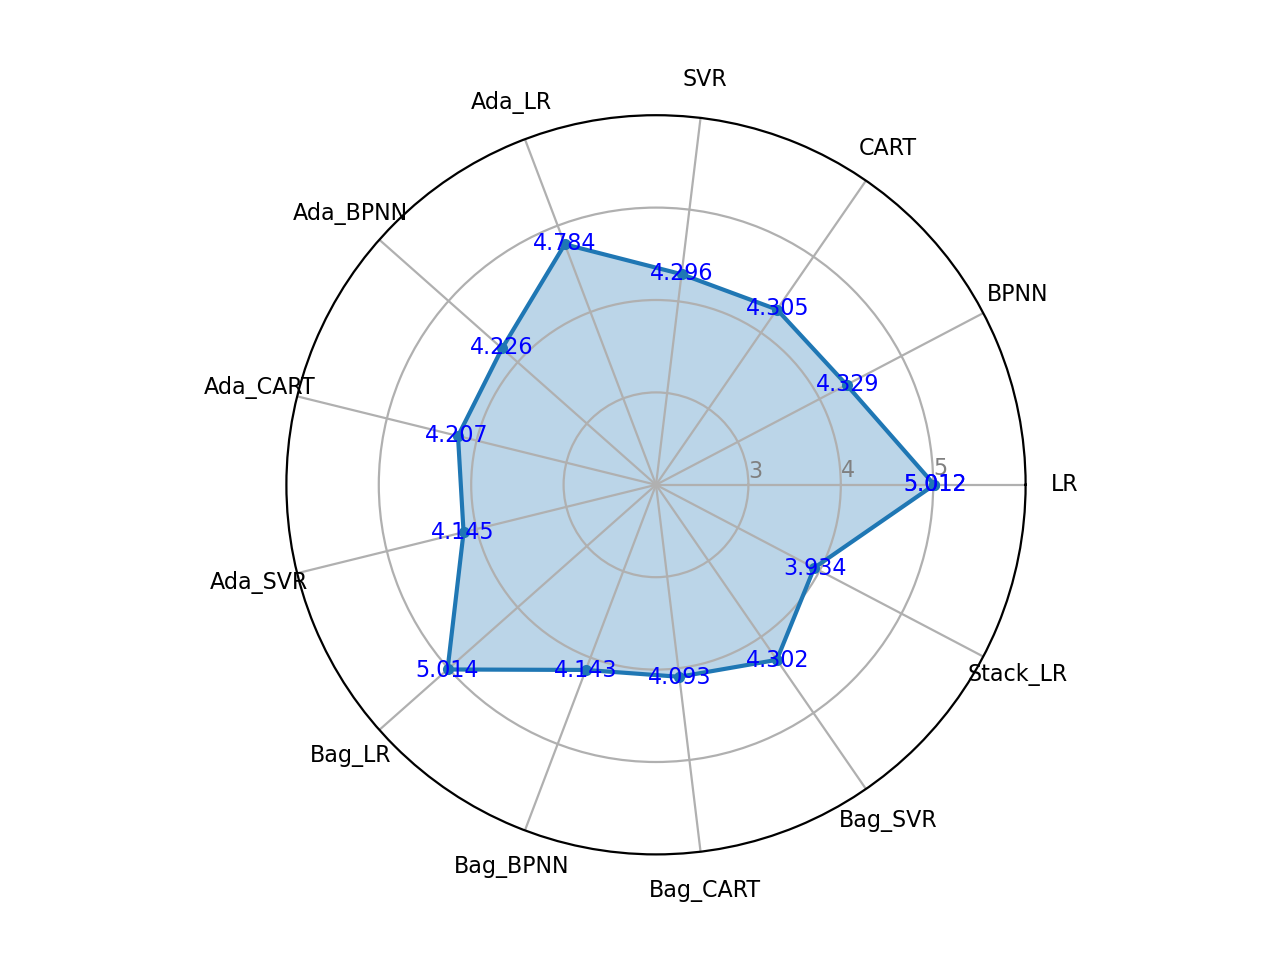
\includegraphics[width = \linewidth]{MAEcircle.png}
			\caption{MAE}
		\end{subfigure}%
		\hspace{-3em}
		\begin{subfigure}{0.53\textwidth}
		\centering
		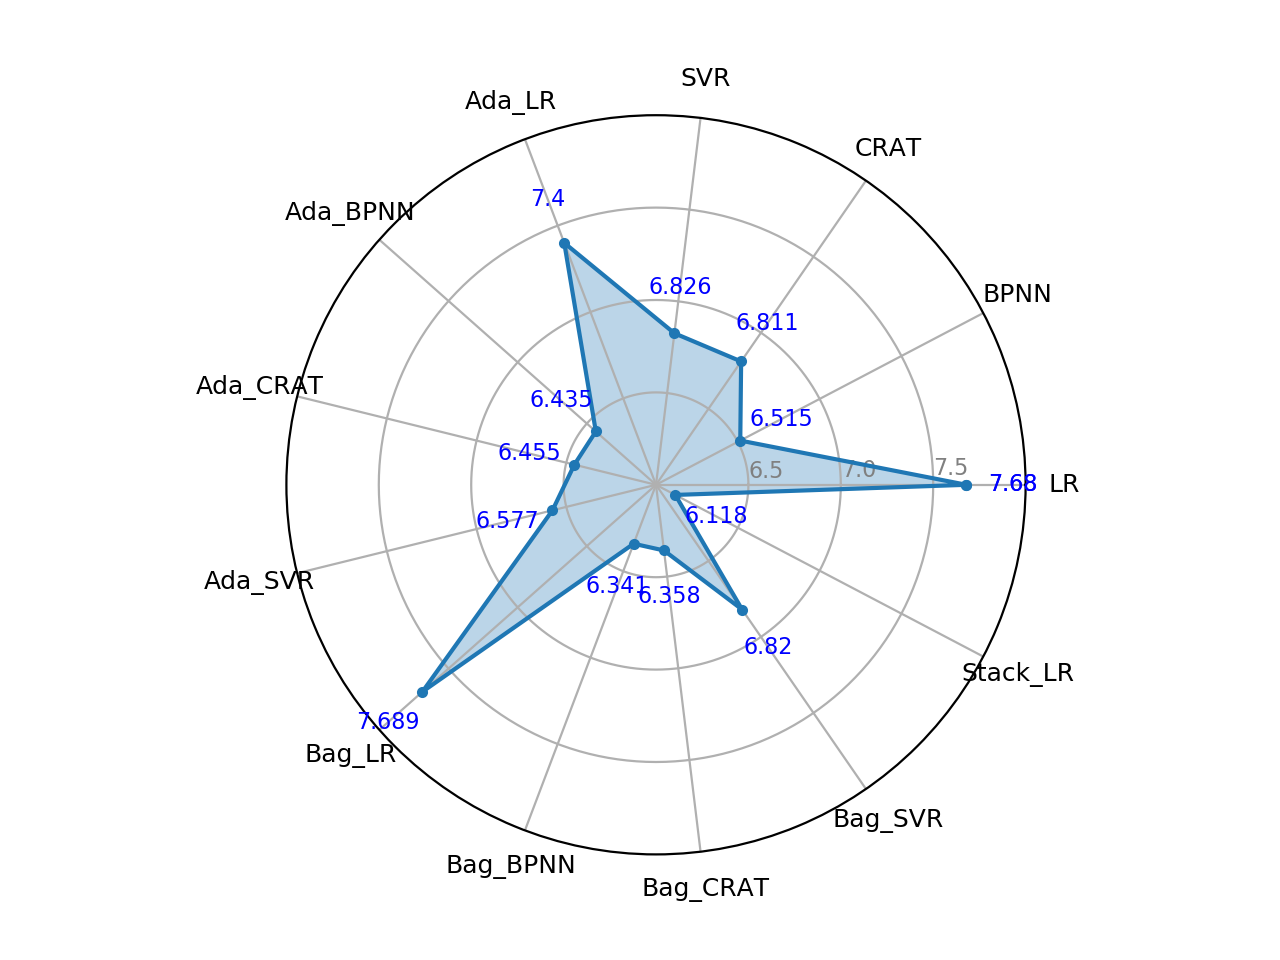
\includegraphics[width = \linewidth]{RMSEcircle.png}
		\caption{RMSE}
		\end{subfigure}%
		\hspace{1em}
		\begin{subfigure}{.53\textwidth}
			\centering
			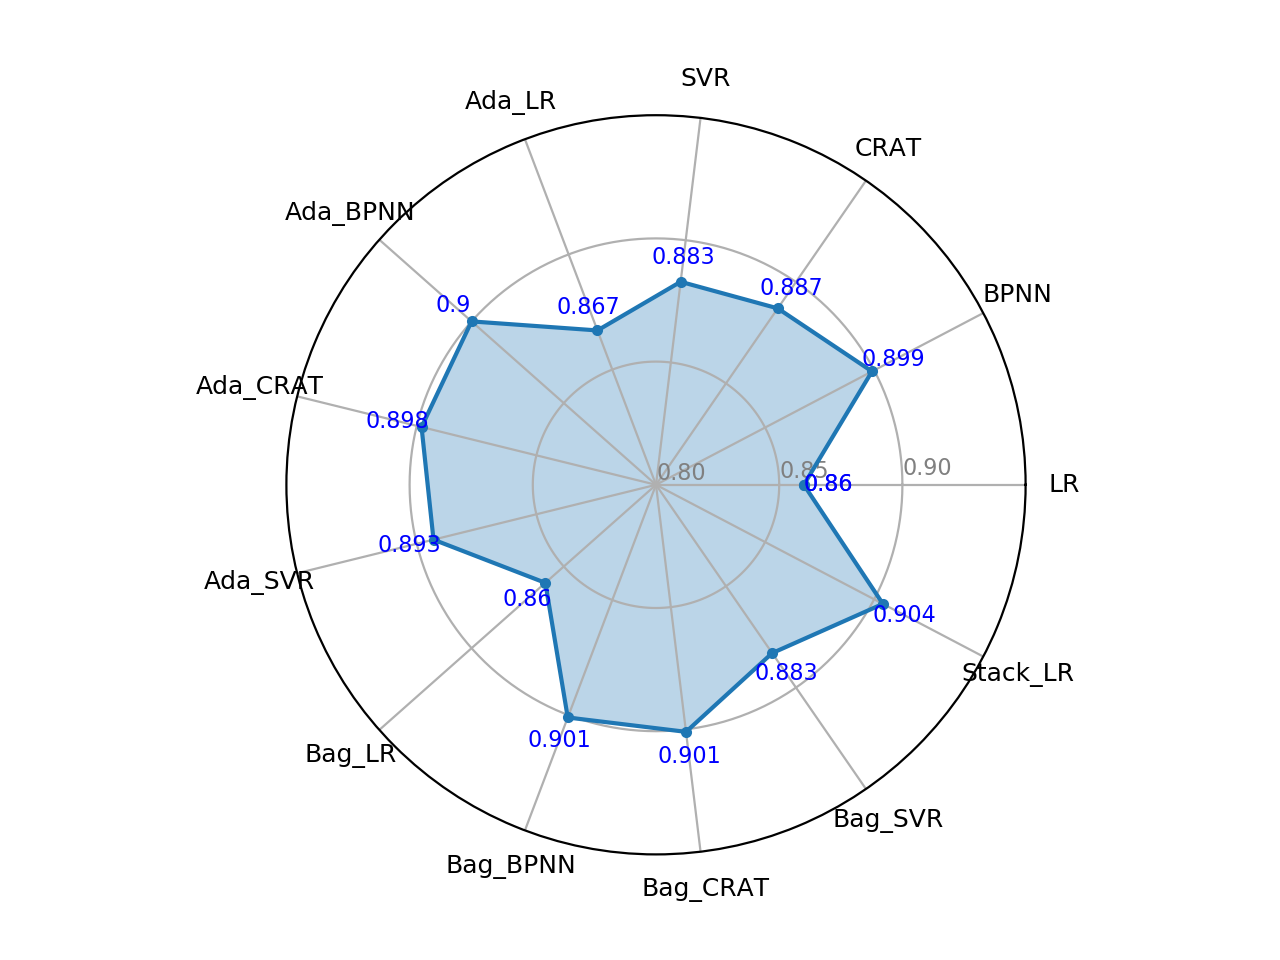
\includegraphics[width = \linewidth]{R2circle.png}
			\caption{$R^2$}
		\end{subfigure}%
		\hspace{1em}
		\caption{Average prediction performance of 10-fold cross-validation on all machine learning models for predicting self-healing ability of ECC }\label{comp}
	\end{figure}
	

	Overall, all models can noticeably reduce the error values and increase the prediction accuracy compared with LR, except Bag\_LR. Among the models boosted by AdaBoost, Ada\_SVR performed the best with the lowest MAE value, whereas Ada\_BPNN performed the best on RMSE value showing the highest $R^2$ value. In case of bagging, both Bag\_CRAT and Bag\_BPNN performed better in terms MAE, RMSE and $R^2$ than those of the corresponding models boosted by AdaBoost. However, Bag\_LR showed a poor performance compared to LR on the MAE and RMSE values. For a better comparison among the ensemble methods used, the performance results between the ensemble models and their corresponding individual (or benchmark) models are indicated in Table \ref{com}. The results indicate that most ensemble methods improved the performance of individual models. For example, the MAE and RMSE values of BPNN after bagging reduced by 4.3\% and 2.7\%, respectively, and with a higher value of $R^2$ compared to those of the individual BPNN model. Among all the ensemble methods studied, stacking showed the best improvement on all performance measures.
	

	
% 	For example, of the models based on ensemble learning by AdaBoost, Ada\_SVR performs the best on MAE, reducing by 17.3\%, Ada\_BPNN performs the best on RMSE, reducing by 16.2\% and on $R^2$, increasing by 4.7\%. For the bagging ensemble methods, Bag\_CRAT performs the best on MAE, reducing by 18.3\%, Bag\_BPNN performs the best on RMSE, reducing by 17.4\%, and Bag\_CRAT and Bag\_BPNN have the same performance on $R^2$, increasing by 4.8\%. However, note that Bag\_LR has a worse performance than LR in terms of MAE and RMSE. This may result from several training examples repeatedly appearing in different replicated datasets to train multiple base regressors. 

% 	Table \ref{com} further shows the deviation of ensemble models from individual models which are used as base learners over the three statistical measures based on ten-fold cross-validation results. The results indicate that the ensemble methods using individual methods as a learning base improved the performance of the individual method on the basis of all three performance measures. For example, using BPNN as the learning base, ensemble method Bag\_BPNN has the lower error (MAE and RMSE decreasing by 4.3\% and 2.7\%, respectively) and higher accuracy ($R^2$ increasing by 0.2\%) than the individual method BPNN. Moreover, the comparative results showed that ensemble learning based models (Stack\_LR) distinctly outperformed the single learning based models (Ada\_LR and Bag\_LR) in terms of overall performance measures.
	
	\begin{table}[!h]
		\small
		\centering
		\caption{Performance deviation of ensemble models from benchmark models on self-healing of ECC }
		\begin{tabular*}{0.9\textwidth}{llccc|llccc}
			\toprule
			&	&	MAE	&	RMSE	&	$R^2$	&	&	&	MAE	&	RMSE	&	$R^2$	\\
			\cmidrule{3-5} \cmidrule{8-10}
			Benchmark & Model& \multicolumn{3}{c|}{$Dev (\%)$} &Benchmark & Model& \multicolumn{3}{c}{$Dev (\%)$} \\
			\midrule
			LR	&	Ada\_LR	&	-4.6	&	-3.6	&	0.8		&	LR	&	Bag\_LR	&	0.0	&	0.1	&	0.0	\\
			BPNN	&	Ada\_BPNN	&	-2.4	&	-1.2	&	0.1	&	BPNN	&	Bag\_BPNN	&	-4.3	&	-2.7	&	0.2	\\
			CRAT	&	Ada\_CRAT	&-2.3	&	-5.2	&	1.2	&	CRAT	&	Bag\_CRAT	&	-4.9	&	-6.6	&	1.6\\
			SVR	&	Ada\_SVR&-3.5	&	-3.6&	1.1	&	SVR	&	Bag\_SVR	&	0.1	&	-0.1	&	0.0	\\
			\midrule
			Ada\_LR	&	Stack\_LR	&	-17.8&	-17.3&	4.3	&	Bag\_LR	&	Stack\_LR	&-21.5	&	-20.4&	5.1 \\
			\bottomrule 
		\end{tabular*}
		\label{com}
	\end{table} 
	
		However, the results showed that the effectiveness of ensemble methods on individual models varied. For instance, bagging method enhanced the performance of BPNN and CRAT substantially, but not for both LR and SVR models. On the other hand, the AdaBoost method brought a considerable improvement for LR and SVR models. To improve the performance accuracy, researchers should employ different ensemble methods to compare their effectiveness on different ML models.  
	
% 	Specifically, bagging ensembles substantially enhance the performance of BPNN and CRAT while the AdaBoost ensemble achieve a considerable improvement for LR and SVR. It means that BPNN and CRAT used as the base learner, bagging method achieves better results (lower error value and higher $R^2$) than the AdaBoost and individual method, and the LR and SVR used as the base learner, the AdaBoost method gets better results than the bagging and individual method.
	
	\subsection{Prediction performance comparison}
% 	\subsubsection{Comparison of MAE}
For assessment of errors between the predicted crack width and the experimental observed crack width, a comparison of the proposed ML models     is illustrated in Figure \ref{error1} to \ref{error4}, in which the predicted crack width after self-healing by ML models and the experimental observed crack width after self-healing are presented in sub-figure (a). Error of predicted crack width over the experimental observed crack width after self-healing is displayed as the measurement index (shown in the vertical coordinate) based on the group of crack width before self-healing (shown in the horizontal coordinate) in the rest of sub-figures. Furthermore, a horizontal line located at the vertical coordinate of zero ($ y = 0$) is marked as the target line in the rest of sub-figures \cite{alshihri2009neural,yan2017evaluation}. Generally, the shorter the error bar (indicates a closer distance from the target line) demonstrates the predicted crack width is more accurate, which means the smaller or even zero error between the predicted crack width and experimental observed crack width after self-healing.
	
% 	preidcted value - observed value.
		\begin{figure}[!h]
		\centering
		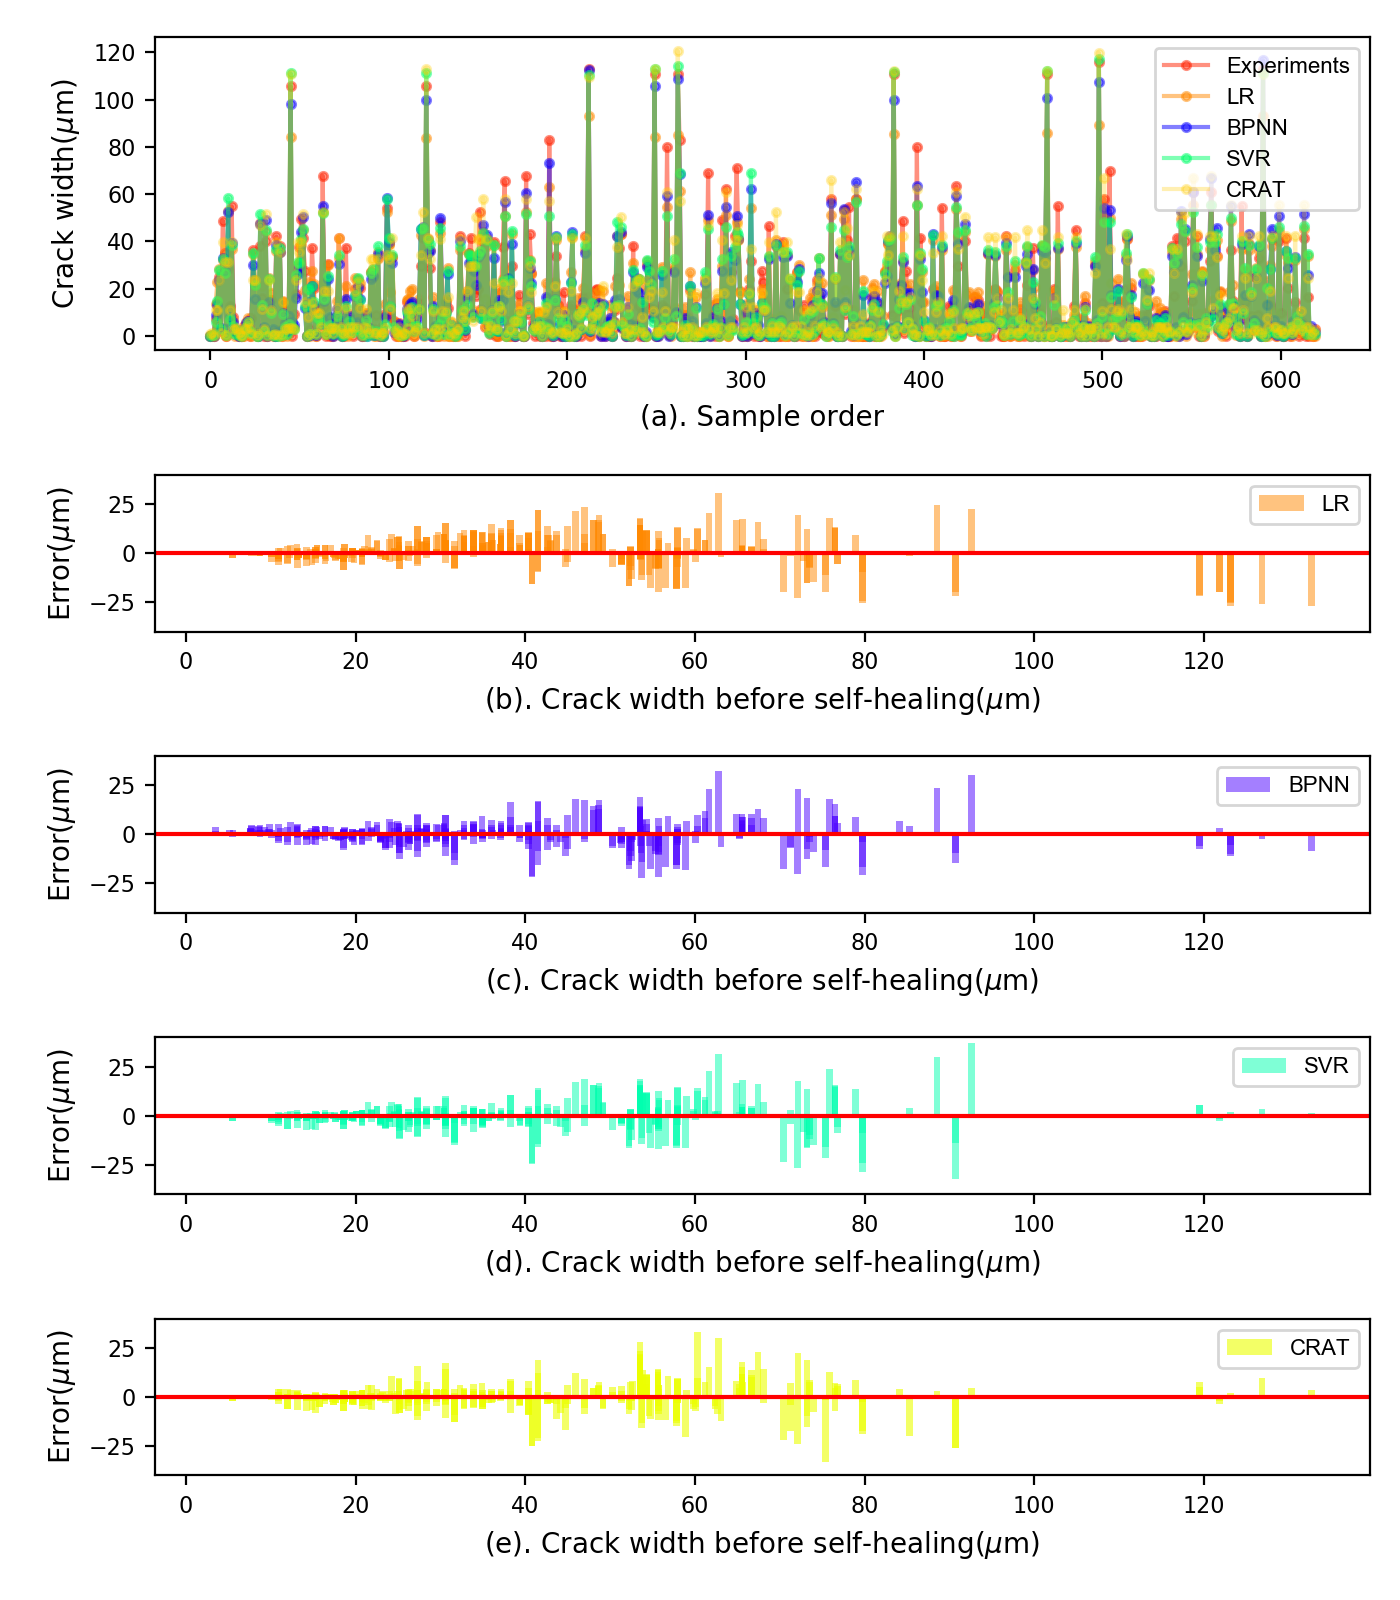
\includegraphics[width=\textwidth]{error.png}
		\caption{Comparison of predicted and observed crack width after self-healing of ECC for individual models}
		\label{error1}
	\end{figure}
	
	\begin{figure}[!h]
		\centering
		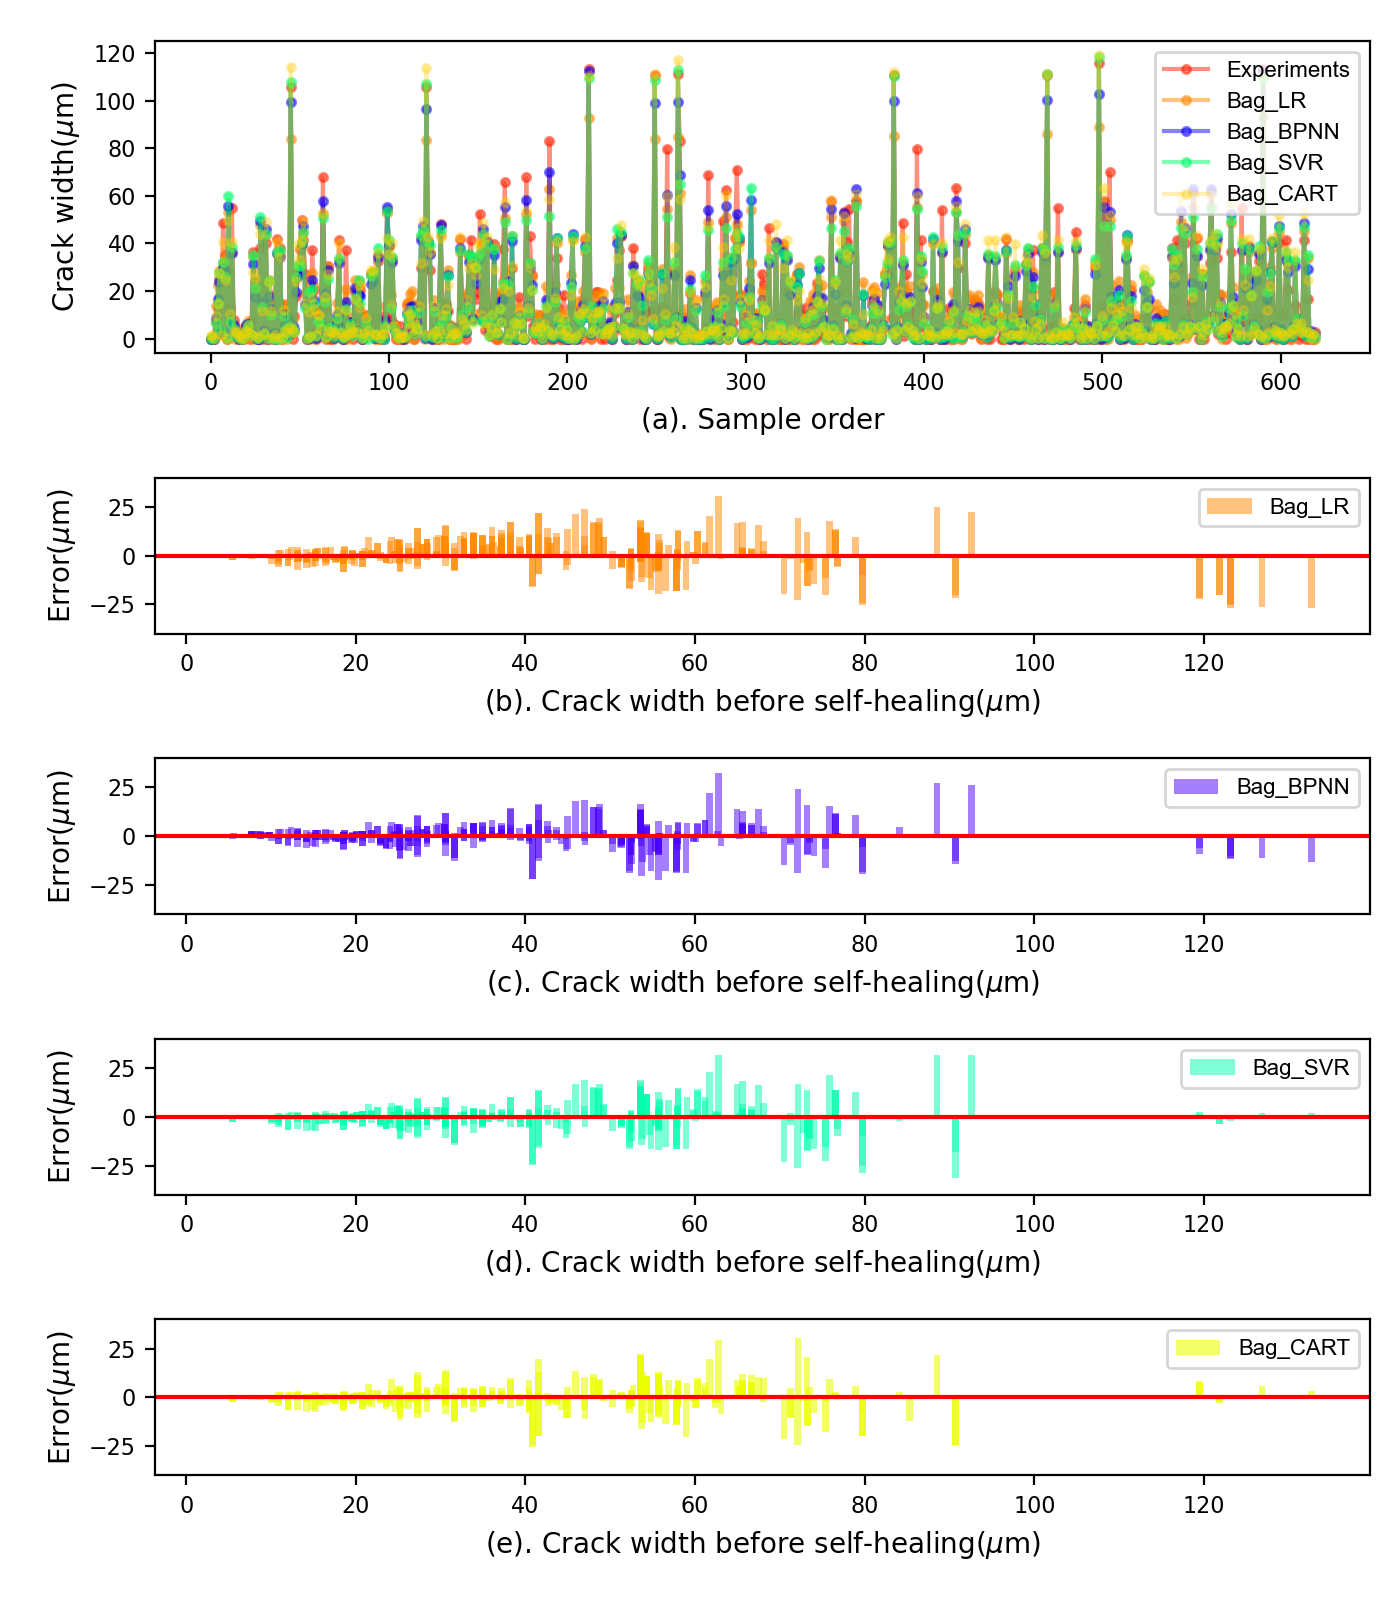
\includegraphics[width=\textwidth]{bagError.png}
		\caption{Comparison of predicted and observed crack width after self-healing of ECC for bagging ensemble models}
		\label{error2}
	\end{figure}
	
		\begin{figure}[!h]
		\centering
		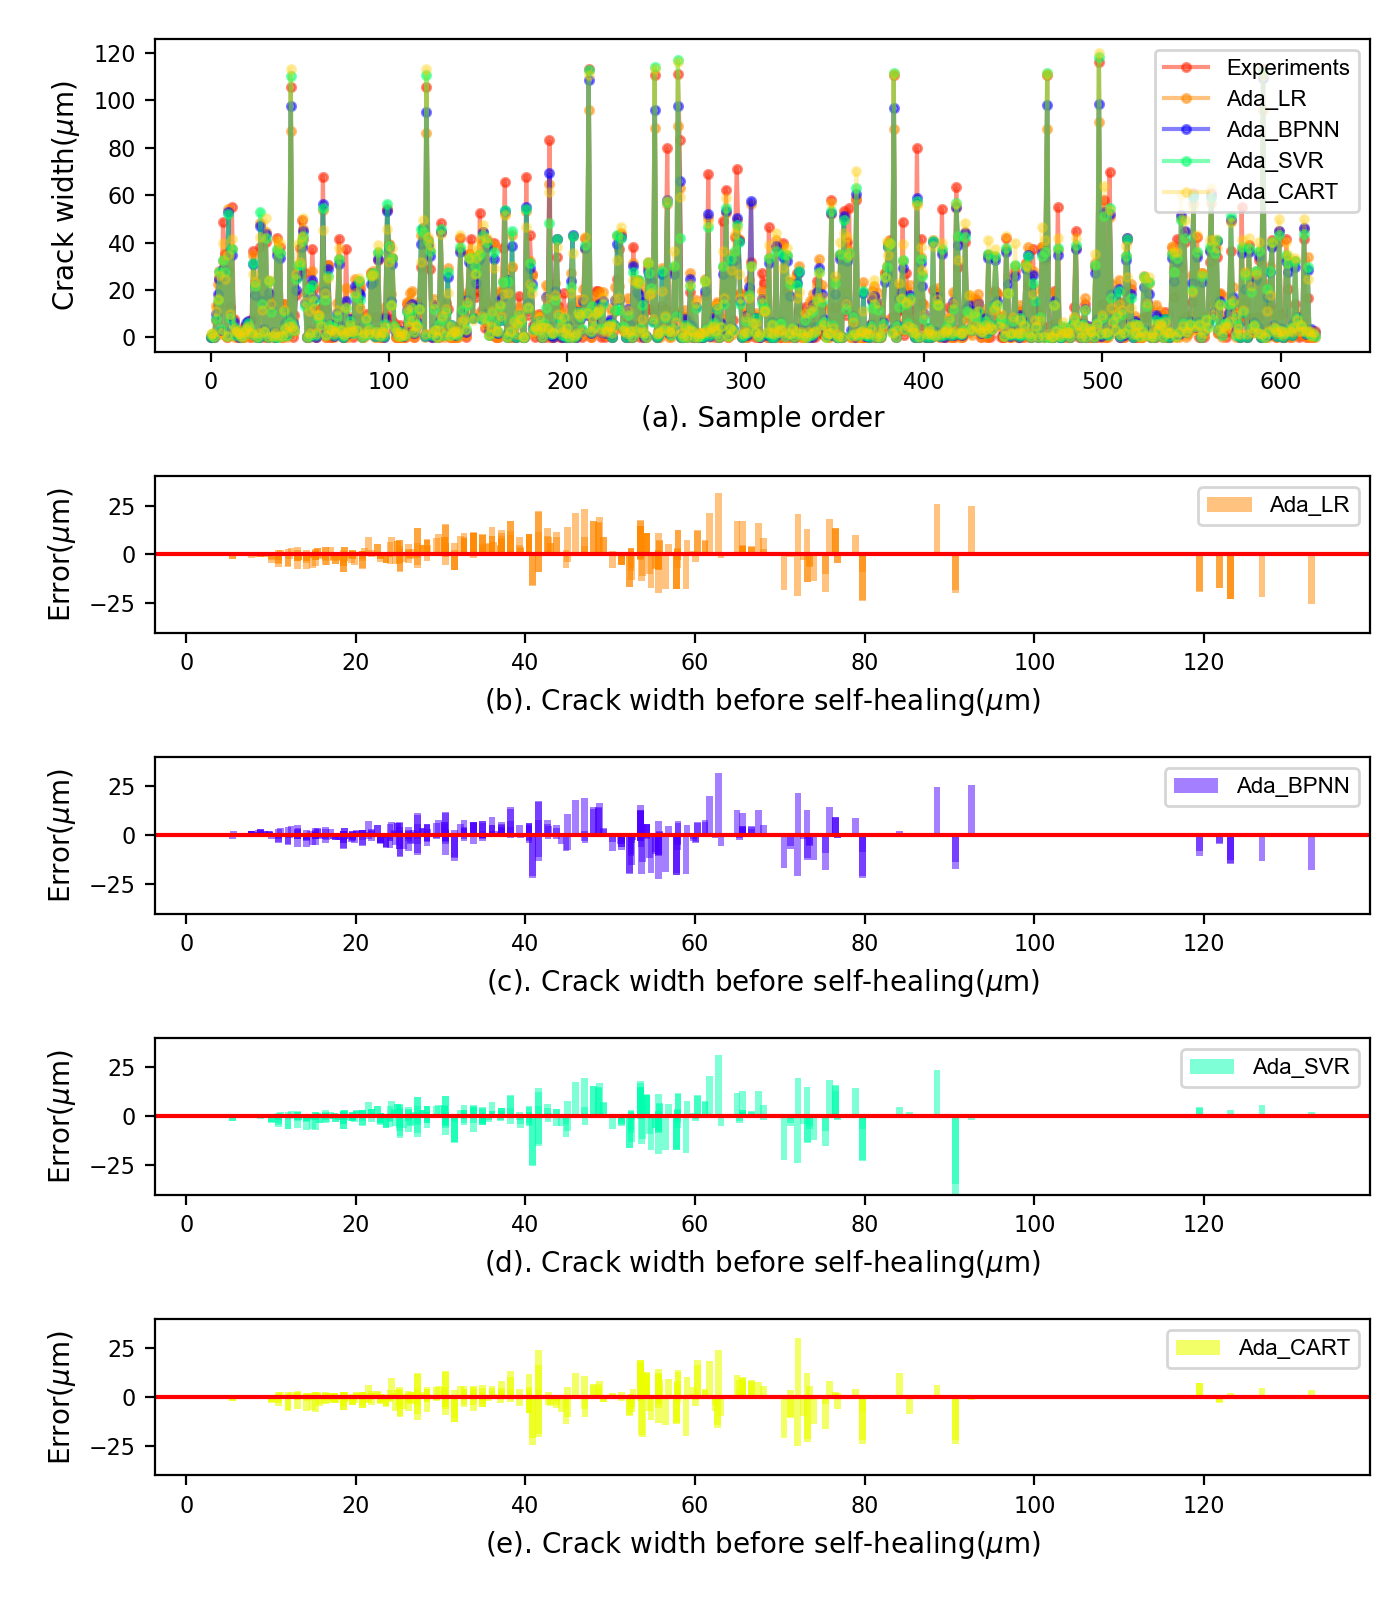
\includegraphics[width=\textwidth]{AdaError.png}
		\caption{Comparison of predicted and observed crack width after self-healing of ECC for adaBoost ensemble models}
		\label{error3}
	\end{figure}

		\begin{figure}[!h]
	\centering
	\includegraphics[width=\textwidth]{StackError.png}
	\caption{Comparison of predicted and observed crack width after self-healing of ECC for stacking ensemble models}
	\label{error4}
\end{figure}

	It has been reported that crack width control is critical to the generation and accumulation of self-healing substances \cite{vidal2004analyzing,wang1997permeability,reinhardt2003permeability,edvardsen1999water,qiu2016coupled} that further affect the self-healing capability of ECC. In order to eliminate the influence of cracking pattern, a newly developed splitting tensile test apparatus (shown in Figure \ref{f:cr1}) was used to control crack width, length and depth, as well as the branched and accumulated crack. As shown in Table \ref{min}, and Figure \ref{error1} to \ref{error4}, the maximum crack width before self-healing is 135.47 $\mu m$ less than 150 $\mu m$, and the majority of cracks are within 100 $\mu m$. Specially, most of the cracks are less than 60 $\mu m$. 

    As shown in Figure \ref{error1}, the SVR model exhibited lower discreteness of error bar than other individual models. For the crack width less than 60 $\mu m$ before self-healing, the variations of the error bar of the SVR model is slightly lower than BPNN and CRAT models, while the CRAT model is slightly lower than SVR and BPNN models for the crack width between 60 and 100 $\mu m$ before self-healing. It is clear that the error bar of SVR model varies slightly around the target line, indicating that the predicted outputs are a little different from the experimental observed crack width and gather around zero for the crack width larger than 100 $\mu m$ before self-healing. Moreover, the variations of the error bar of SVR model is lower than CRAT model which is lower than BPNN model. And all three models exhibit lower error bar variation than the LR model that demonstrates substantial deviation from the target line (denoting relative larger differences between the predicted crack width and the experimental observed crack width). This is consistent with the model indicator MAE analysed in Table \ref{per}. Among the individual models, the MAE between the predicted crack width and the experimental observed crack width is 4.296 for SVR that is lower than BPNN (4.329) and CRAT (4.305) models, and all of them is lower than LR (5.012) model as shown in Table \ref{per}.
    
    	

	
    From Figure \ref{error2} and \ref{error3}, we can see that the bag\_CRAT and Ada\_CRAT models exhibited lower error derivation from the target line than other ensemble models. It is clear that the variation of error bar of bag\_CRAT and Ada\_CRAT models are limited within a shorter interval, especially for the crack width between 60 and 100 $\mu m$ before self-healing. Meanwhile, the error bar of these two ensemble models oscillated slightly than CRAT model. The MAE between the predicted crack width and the experimental observed crack width is 4.093 of bag\_CRAT and 4.207 of Ada\_CRAT. However, the variations of error bar of BPNN compared with Ada\_BPNN and bag\_BPNN, and of SVR compared with Ada\_SVR and bag\_SVR don't exhibit distinct differences. As it can be seen in Figure \ref{error4}, the variations of the error bar of stack\_LR model exhibits limited interval $[-20,20]$ while all other models shown $[-25,25]$. The MAE between the predicted crack width and the experimental observed crack width is 3.934. 
    
    
    It is known that the self-healing performance increase with the decrease in crack width \cite{herbert2013selfhealing,liu2017influence}, this may due to the fact that small cracks consume less repair products to complete self-healing processes \cite{de2018review}. That means larger crack width before self-healing potentially has larger crack width after self-healing, which usually exhibit higher error between the predicted crack width and the experimental observed crack width after self-healing. As shown in Figure \ref{error1} to \ref{error4}, all individual and ensemble models exhibit slightly oscillation around the target line for crack width less than 60 $\mu m$ before self-healing, and this oscillation increases as the crack width increases for the crack under 100 $\mu m$. For the crack width over 100 $\mu m$, LR, bag\_LR and Ada\_LR models are in line with this increasing processes, which show larger oscillation interval. However, this oscillation interval decreases for all other ML models in the group of crack width over 100 $\mu m$. 
    
    Thus, it can be concluded that the accuracy of the LR method is significantly improved by BPNN, CRAT and SVR methods by either using individual models or using ensemble models. And the stack\_LR model that combines multiple prediction models (BPNN, CRAT, SVR and LR) is superior to all other models shown the lowest error discreteness. 
	
% 	Table \ref{per} shows the average performance of ten-fold cross-validation for each model (in each row), and the performance deviation from the LR model with respect to MAE, RMSE and $R^2$, respectively. 
	
% 	As it can be seen, Stack\_LR is superior to all other individual or ensemble models on the basis of all three performance measures. 
	
% \subsubsection{Comparison of RMSE}
	In order to assess the RMSE of ten-fold cross validation, the distribution of RMSE calculated based on the differences between the predicted crack width and experimental observed crack width after self-healing is presented graphically in Figure \ref{bar} as a boxplot. Box plot is a statistical tool that is used to 
	depicting numerical data through their quartiles including maximum, minimum, median values of a dataset \cite{taffese2015caprm,olalusi2020machine}.The medium value is shown as the red line whitin the box. Each rectangular box indicates the interquartile range (IQR) covers the 50\% (the lower 25\% to the upper 75\% quartiles) of the RMSE data point, while the whiskers drawn up and down to the maximum and nimimum values represented 1.5 times the IQR from the RMSE data. All other points out of the whiskers range are outliers and shown as red plus sign. A mean value of RMSE equal to zero would indicate a perfect model that achieves a perfect fit between the predicted crack width and the experimental observed crack width. In general, the perfect condition almost never achieved in practice \cite{wikiRMSE}, and a lower RMSE value indicates a better prediction performance of a model. 
   	
	
	Assessment of the box plot revealed that the stack\_LR has the smallest median value (6.118 shown in Table \ref{per}) and the shortest length of the IQR of all the ML models, thereby suggesting minor variation of RMSE for the stack\_LR model. In contrast, the LR and bag\_LR have the largest median value (7.680 and 7.689 shown in Table \ref{per}) and longest length of the IQR of all the ML models, thereby suggesting considerable variation of RMSE for the LR and its ensemble models. Regarding the individual models, the BPNN has the lowest median value of RMSE, the SVR model has the shortest length of the IQR but three outliers (of ten data points), and all three models have lower median RMSE value than LR. Regarding the adaBoost and bagging ensemble models, BPNN, CRAT and SVR have lower median RMSE value than LR, and the SVR has the shortest length of IQR but with outliers. 
	
	Therefore, it can be concluded that the stack\_LR outperforms all other models, which has the lowest median and smallest variation of RMSE, suggesting the best fit of predicted crack width and the experimental observed width. Regarding the rest of ML models, the BPNN display the most stable performance in either individual models or ensemble models with reasonable low median value and short IQR of all other models. 
	
	
	\begin{figure}[!h]
		\centering
		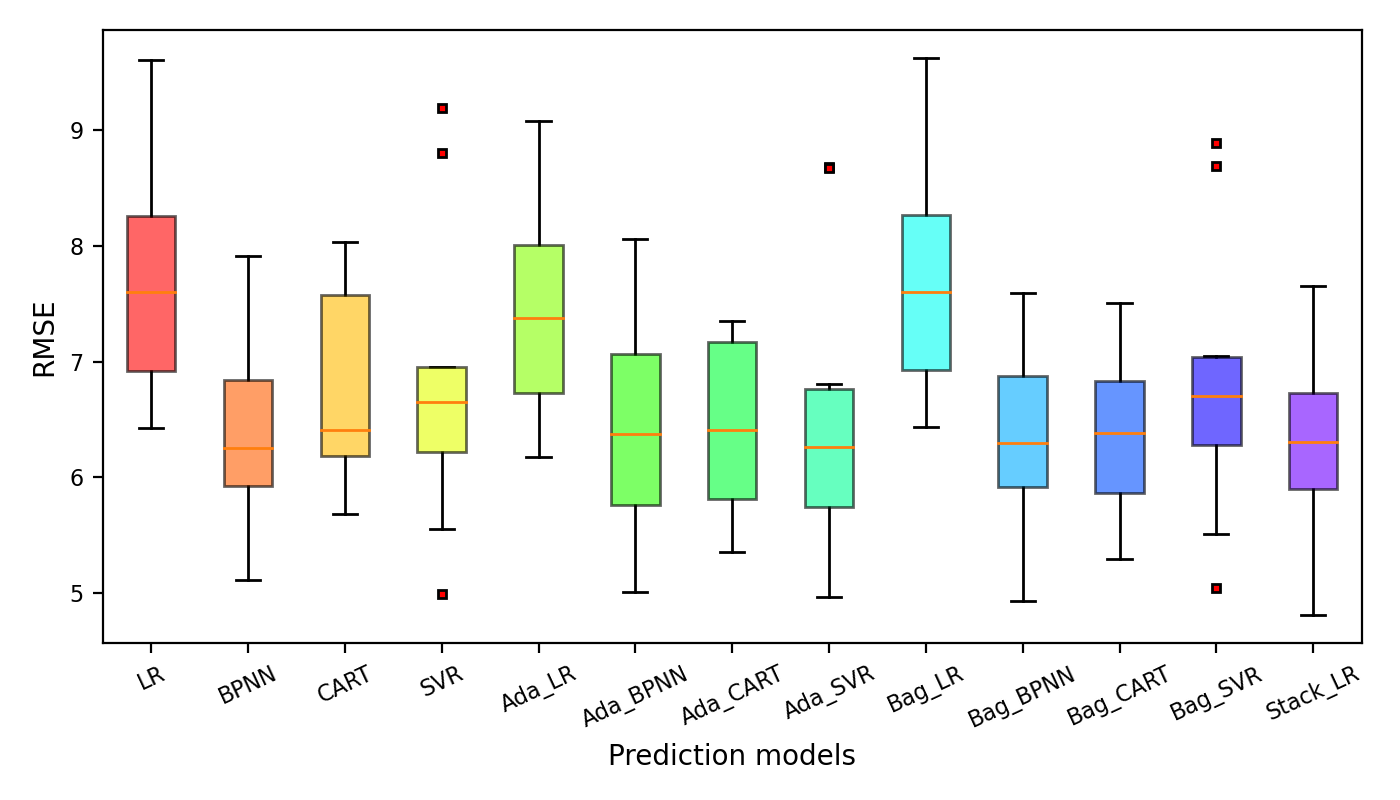
\includegraphics[width=\textwidth]{boxRMSE.png}
		\caption{Ten-fold cross validation of RMSE by proposed ML models in prediction of self-healing ability of ECC}
		\label{bar}
	\end{figure}
	

% \subsubsection{Comparison of $R^2$}	
	In the following, the linear regressions of the predicted crack width and experimental observed crack width after self-healing (after 10 W/D cycles) are evaluated using $R^2$ as illustrated in Figure \ref{gbrt} and \ref{fig:st}. The coefficient of determination $R^2$ and equation of the linear least square fit line are shown in the Figure (of the form $y = ax +b$ relating predicted crack width $``y"$ after self-healing which is the dependent variable to experimental observed crack width $``x"$ after self-healing as an independent variable) indicates that the prediction output is very close to the experimental observed results. Basically, $R^2$ interpreted the correlation, not accuracy \cite{khanal2018integration}. Although a high $R^2$ value would not lead to accurate prediction of a model, the more closely the $R^2$ approaches to one, and with the slope $``a"$ of the fit line is closer to 1 and the $``y"$ intercept $``b"$ is more small, close to 0 (the fit line is more close to the target line $Y = X$), the better the prediction performance is achieved. 
	
	
	\begin{figure}[!h]
		\centering
		    \begin{subfigure}{.35\textwidth}
			\centering
			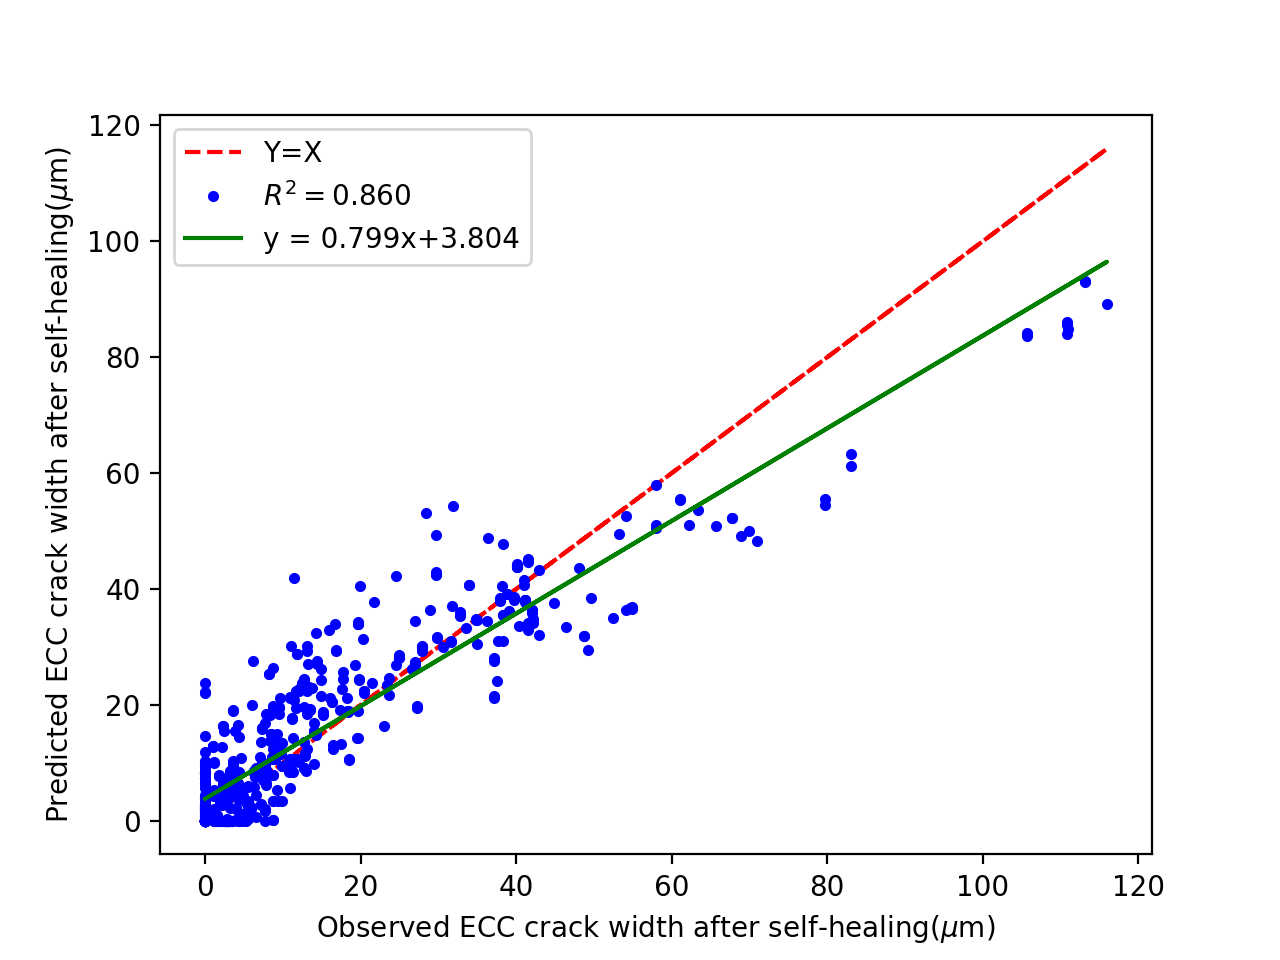
\includegraphics[width = \linewidth]{02LR.png}
			\caption{LR}
		    \end{subfigure}%
		\hspace{-1.4em}
			\begin{subfigure}{.35\textwidth}
		    \centering
		    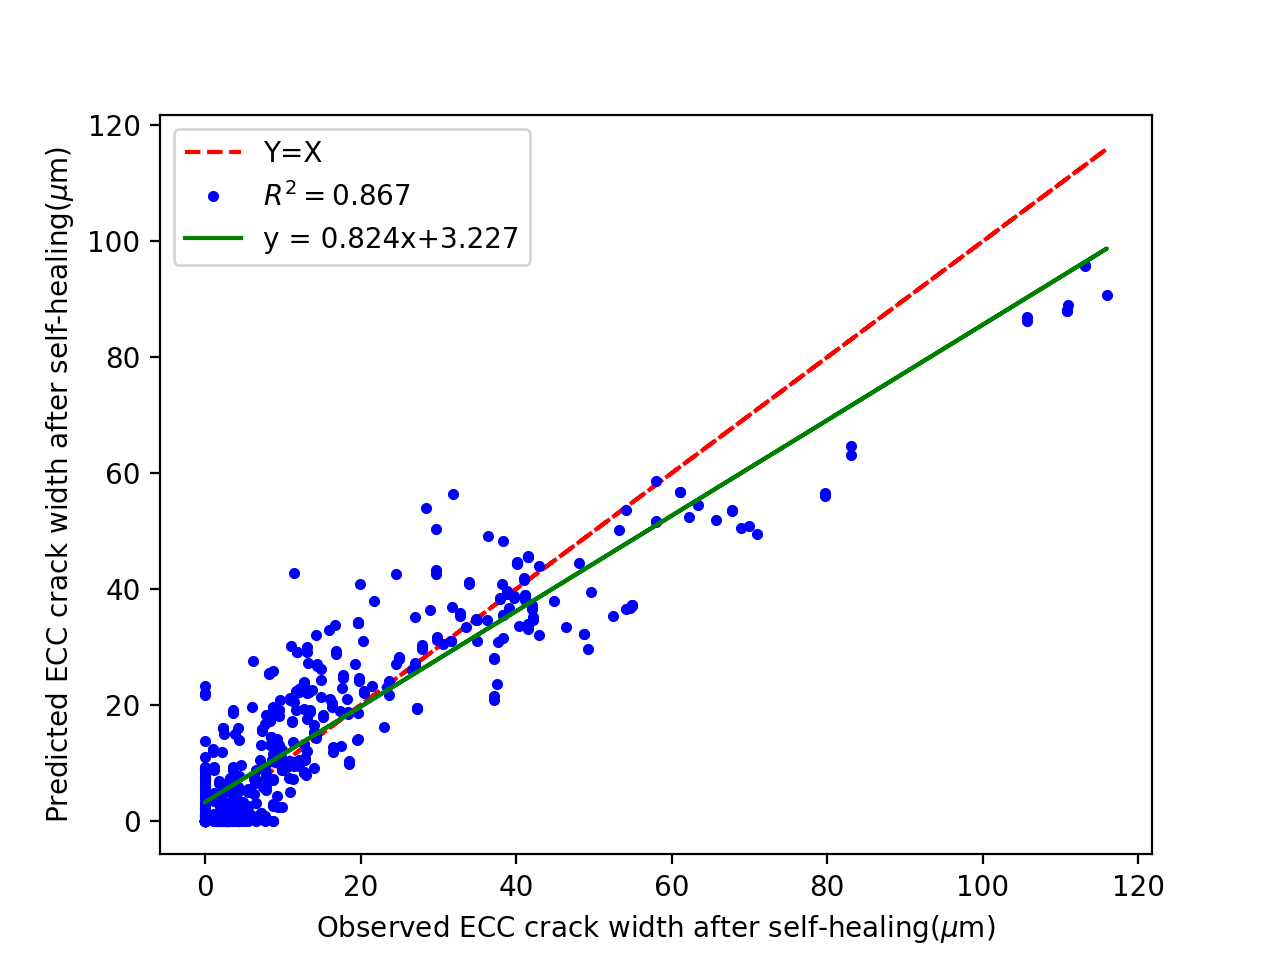
\includegraphics[width = \linewidth]{02Ada_LR.png}
		    \caption{Ada\_LR}
		    \end{subfigure}%
		\hspace{-1.4em}
		    \begin{subfigure}{.35\textwidth}
		    \centering
		    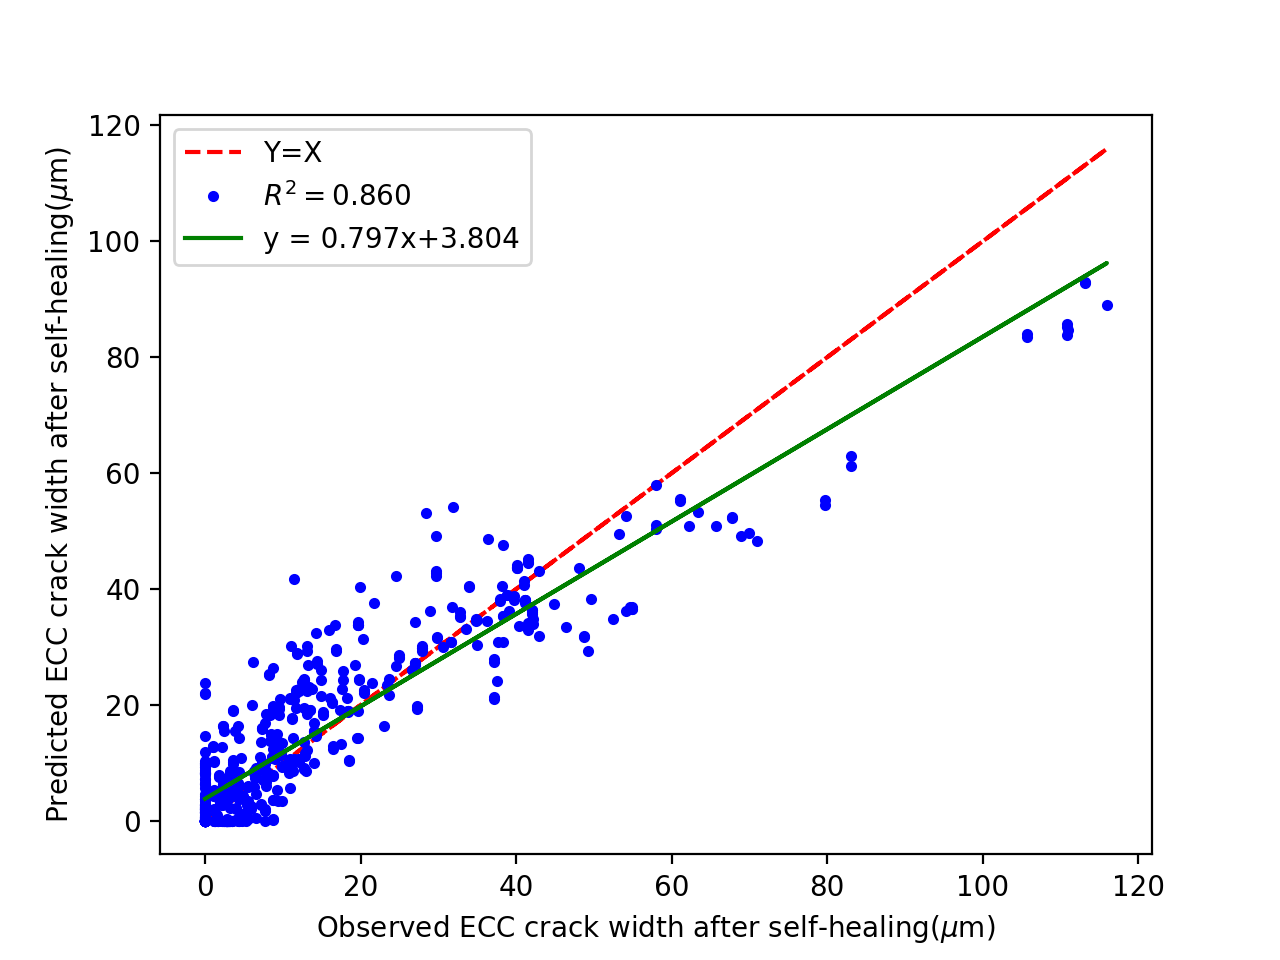
\includegraphics[width = \linewidth]{02Bag_LR.png}
		    \caption{Bag\_LR}
	    	\end{subfigure}%
		\hspace{-1.4em}
		    \begin{subfigure}{0.35\textwidth}
		    \centering
		    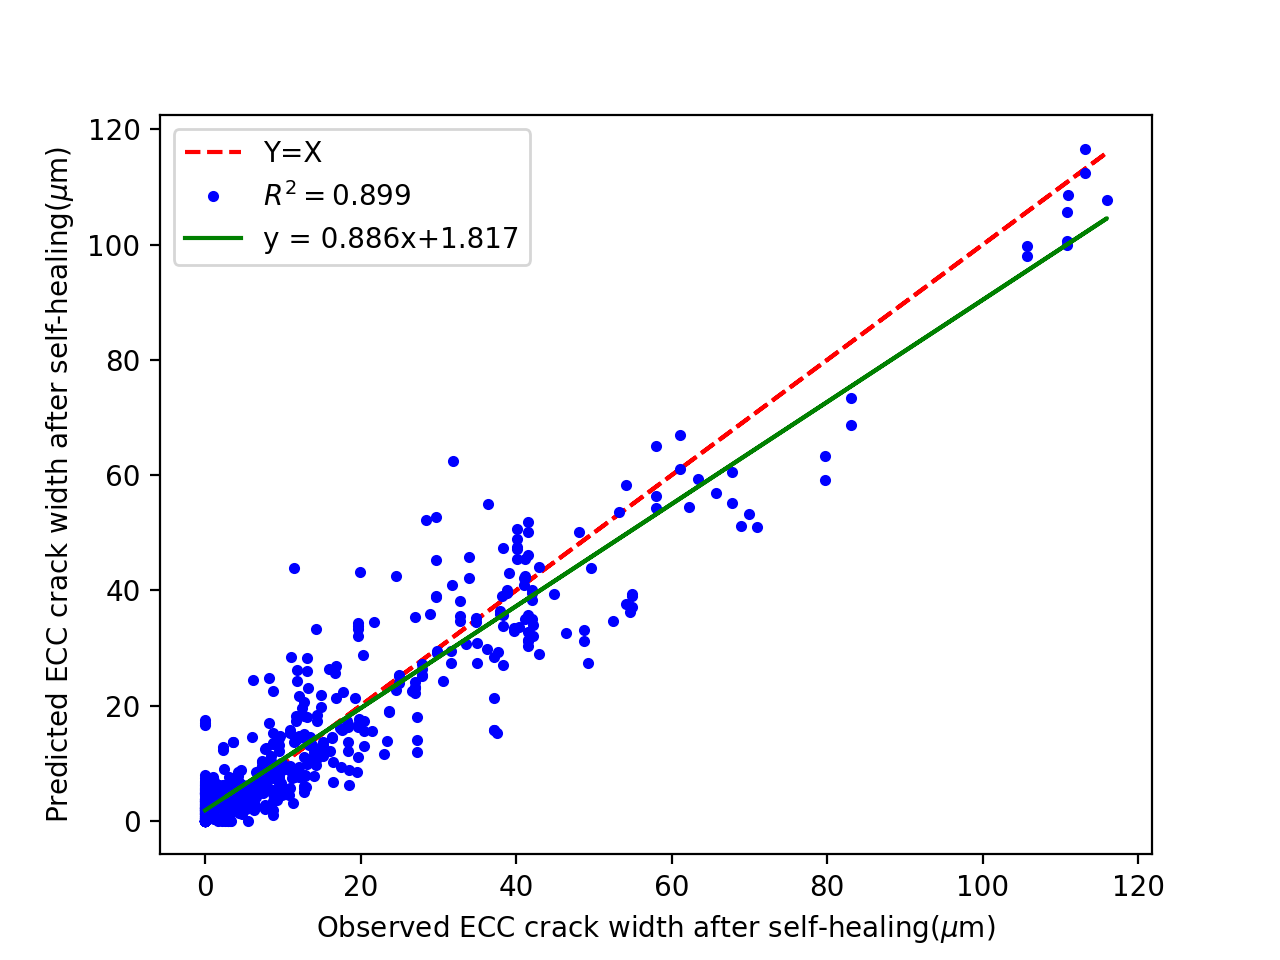
\includegraphics[width = \linewidth]{02BPNN.png}
		    \caption{BPNN}
		    \end{subfigure}%
		\hspace{-1.4em}
		    \begin{subfigure}{0.35\textwidth}
		    \centering
		    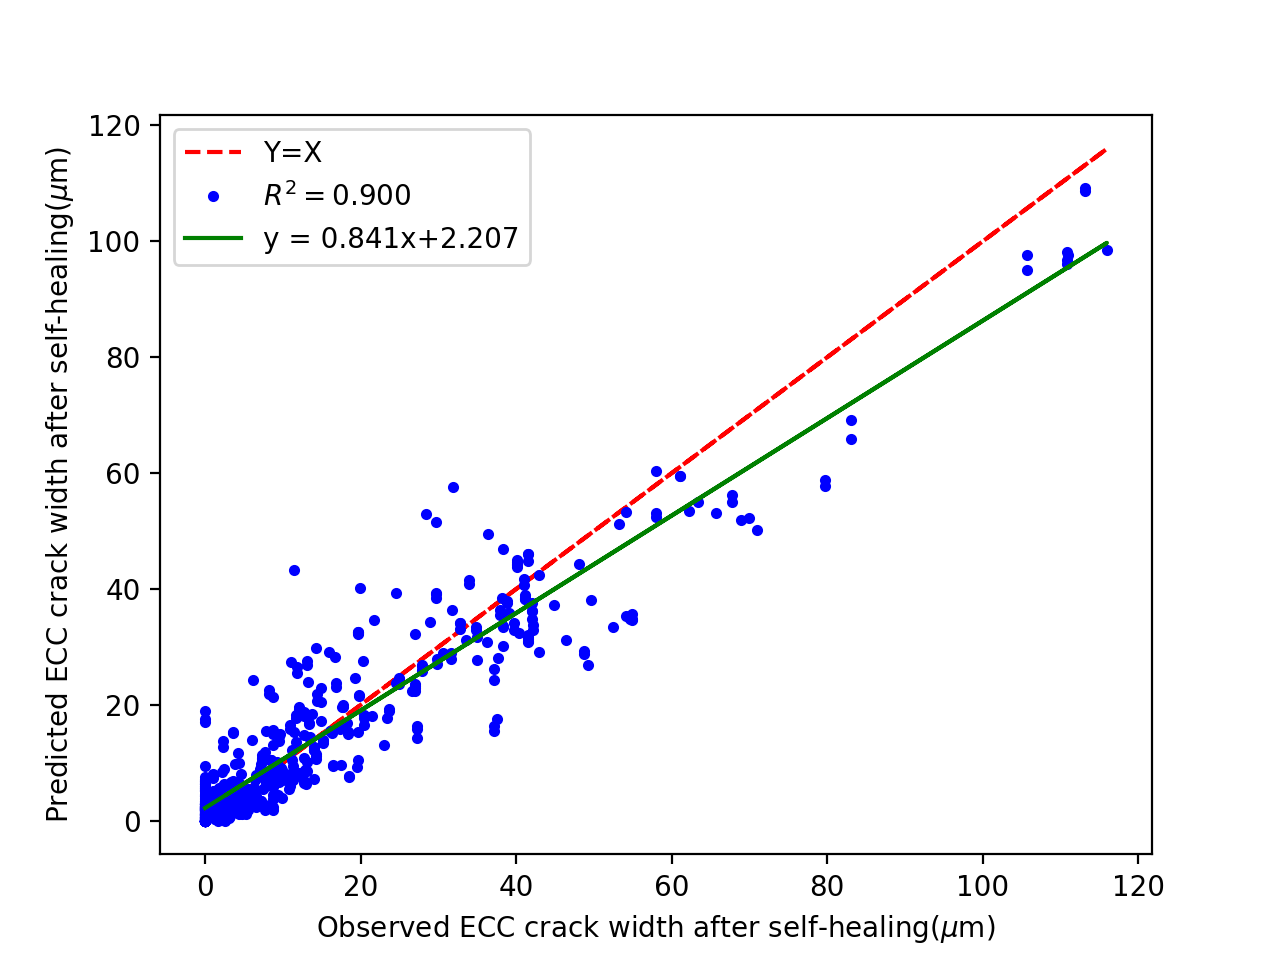
\includegraphics[width = \linewidth]{02Ada_BPNN.png}
		    \caption{Ada\_BPNN}
		    \end{subfigure}%
		\hspace{-1.4em}
		    \begin{subfigure}{0.35\textwidth}
		    \centering
		    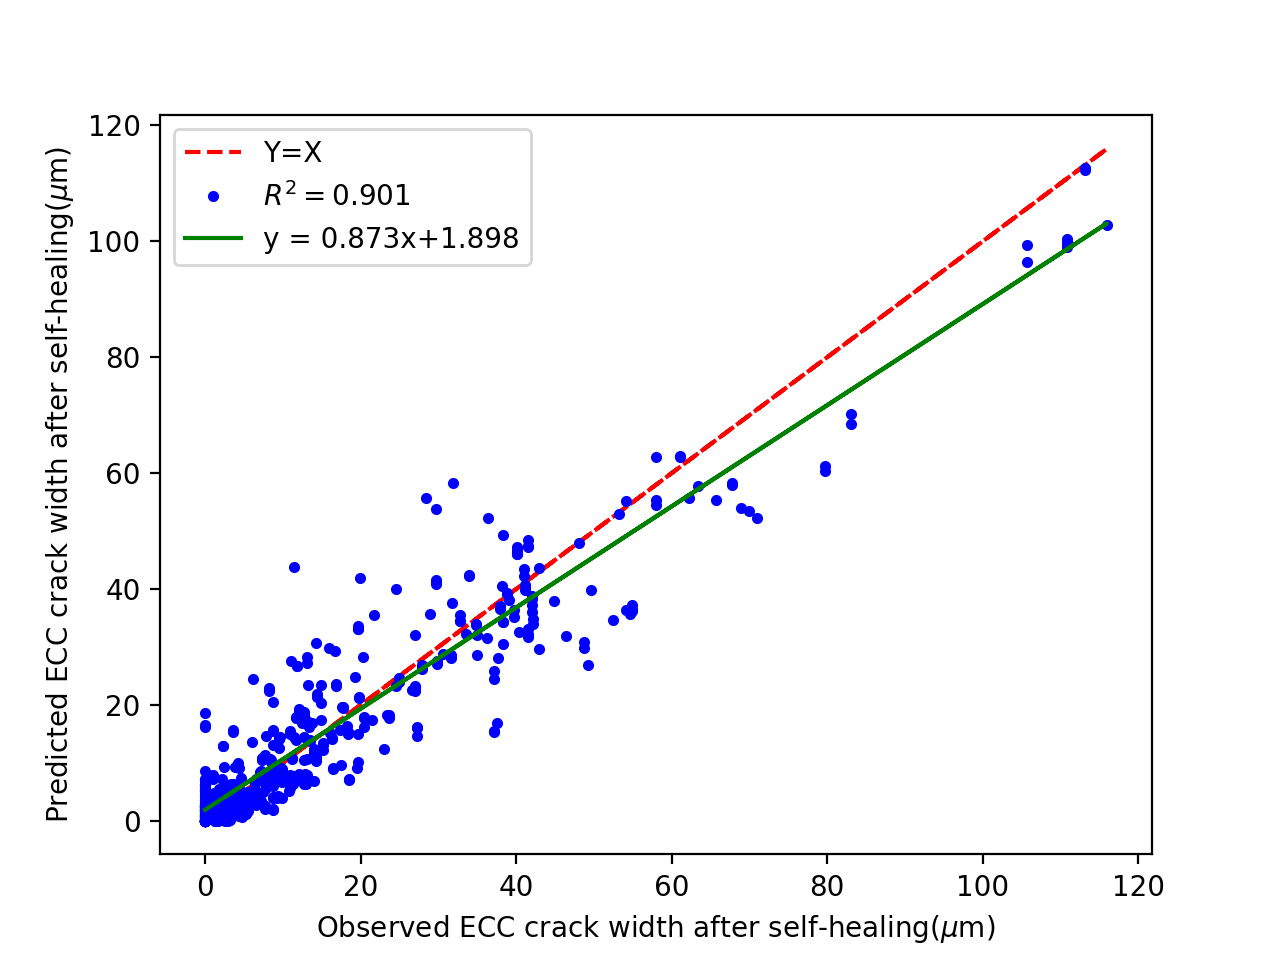
\includegraphics[width = \linewidth]{02Bag_BPNN.png}
		    \caption{Bag\_BPNN}
		    \end{subfigure}%
		\hspace{-1.4em}
		    \begin{subfigure}{.35\textwidth}
			\centering
			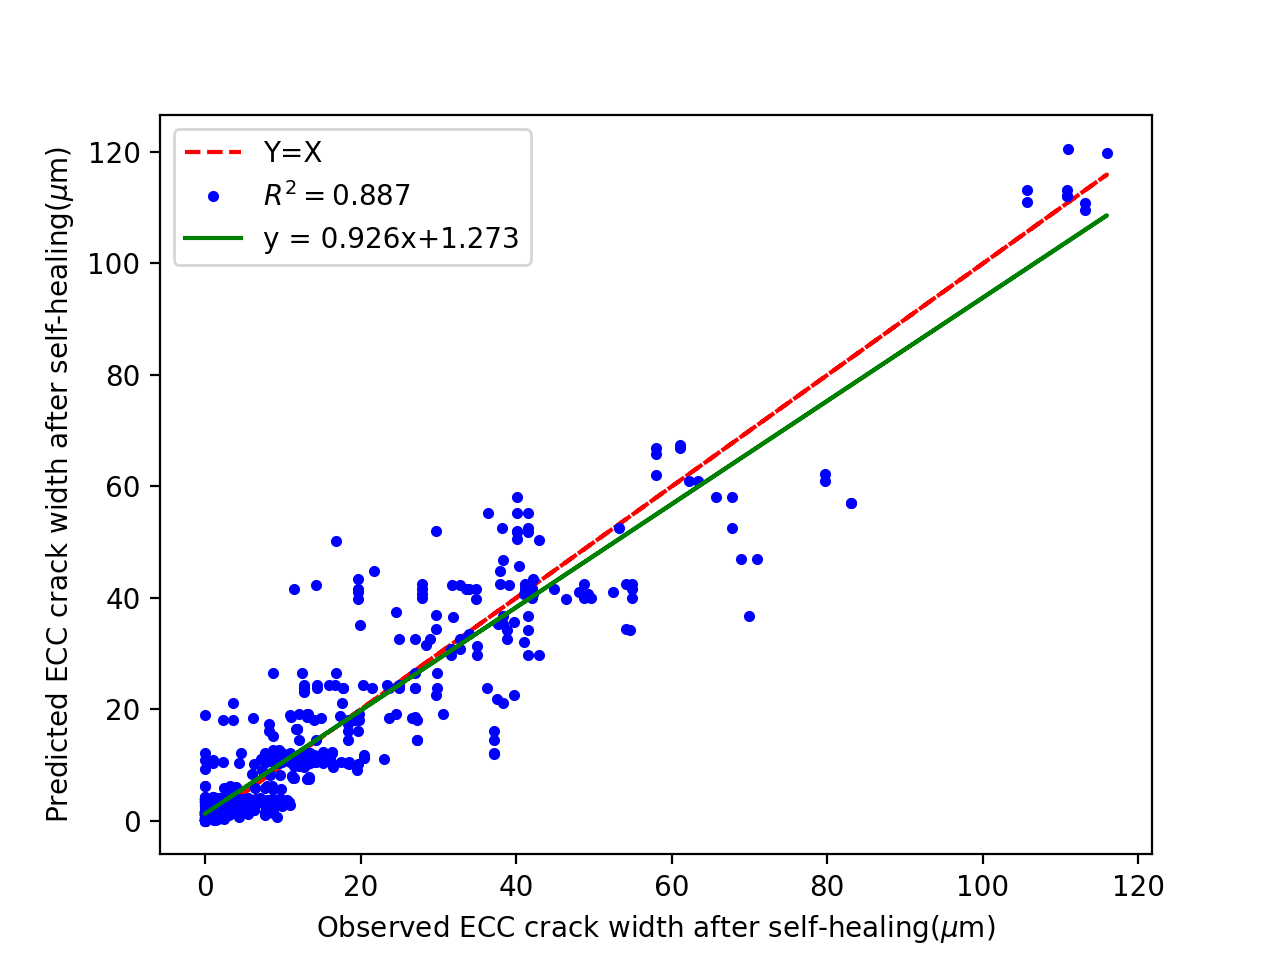
\includegraphics[width = \linewidth]{02CRAT.png}
			\caption{CRAT}
		    \end{subfigure}%
		\hspace{-1.4em}
		    \begin{subfigure}{.35\textwidth}
			\centering
			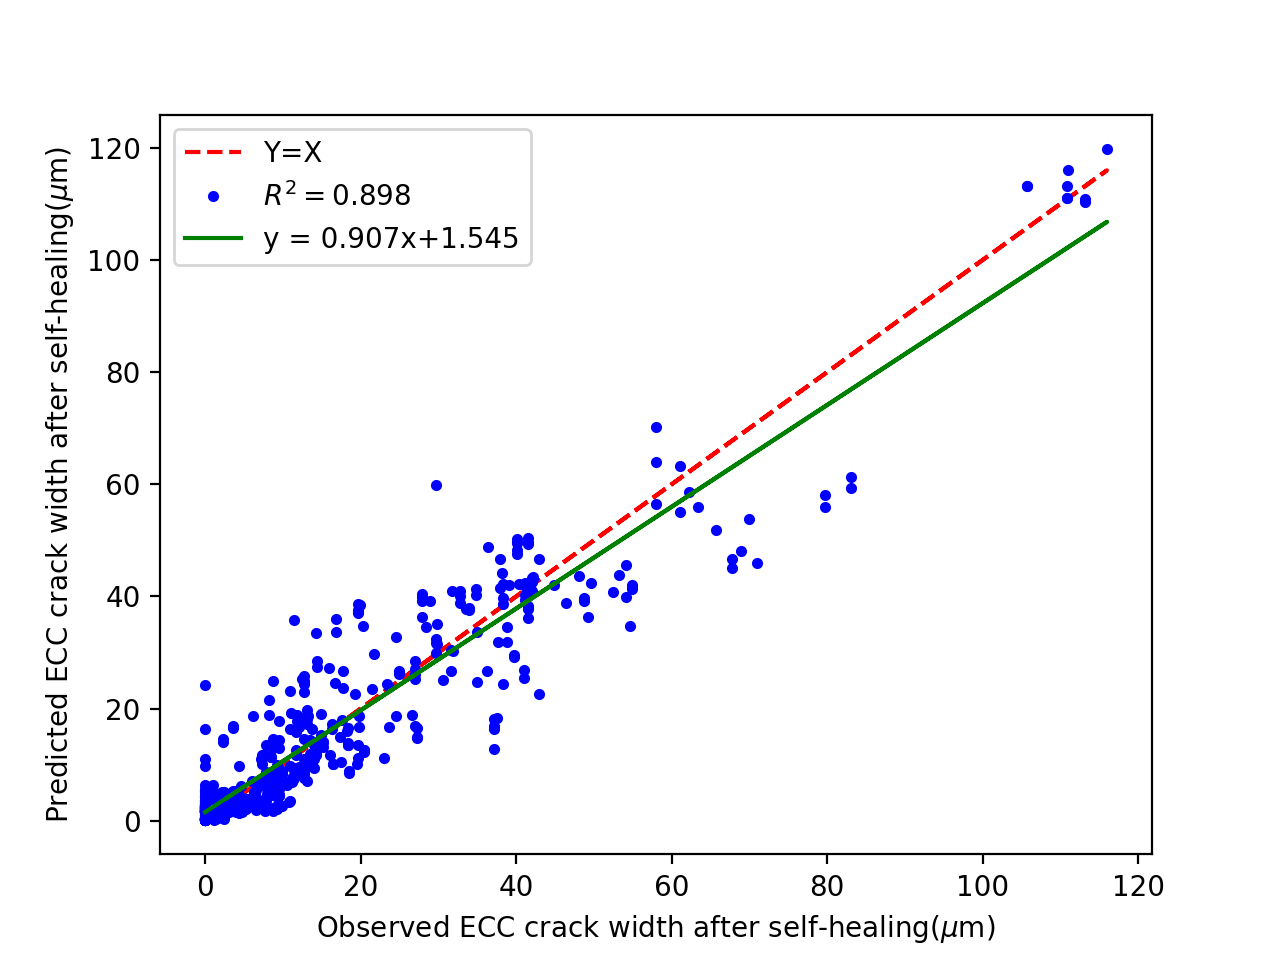
\includegraphics[width = \linewidth]{02Ada_CRAT.png}
			\caption{Ada\_CRAT}
		    \end{subfigure}%
		\hspace{-1.4em}
		    \begin{subfigure}{.35\textwidth}
			\centering
			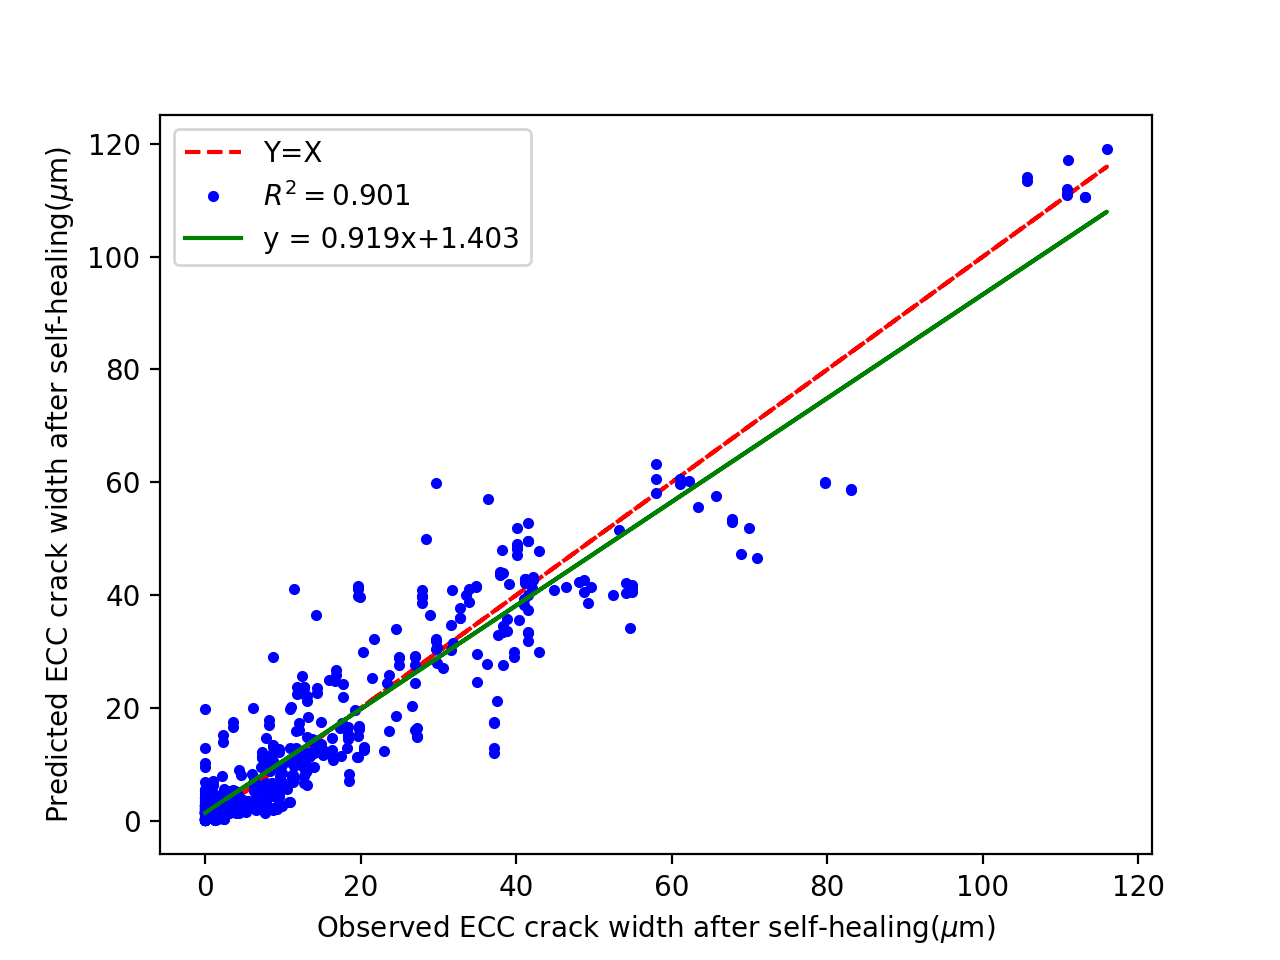
\includegraphics[width = \linewidth]{02Bag_CRAT.png}
			\caption{Bag\_CRAT}
		    \end{subfigure}%
		\hspace{-1.4em}
		    \begin{subfigure}{0.35\textwidth}
		    \centering
		    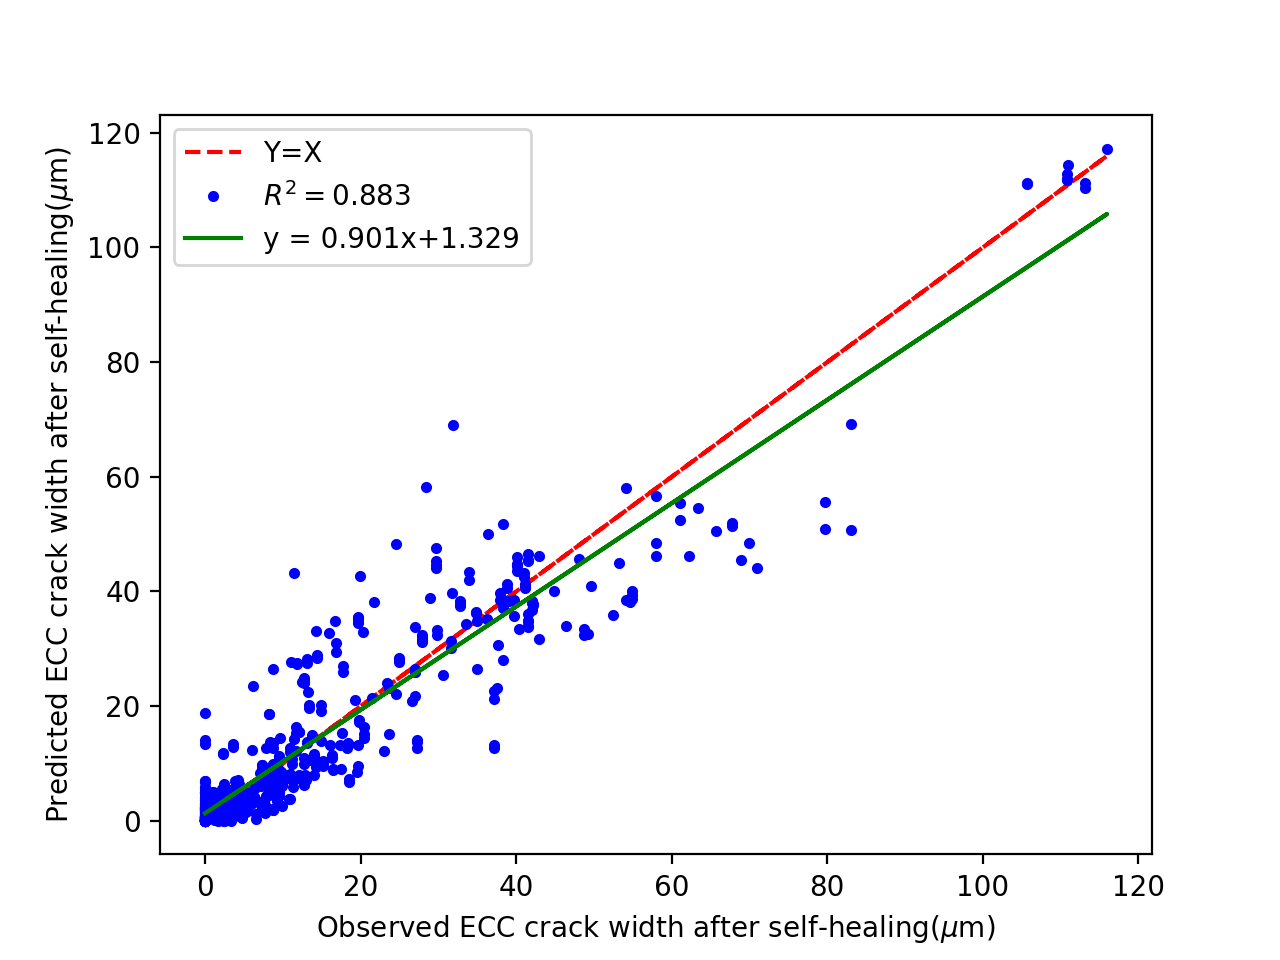
\includegraphics[width = \linewidth]{02SVR.png}
		    \caption{SVR}
		    \end{subfigure}%
		\hspace{-1.4em}
	    	\begin{subfigure}{.35\textwidth}
			\centering
			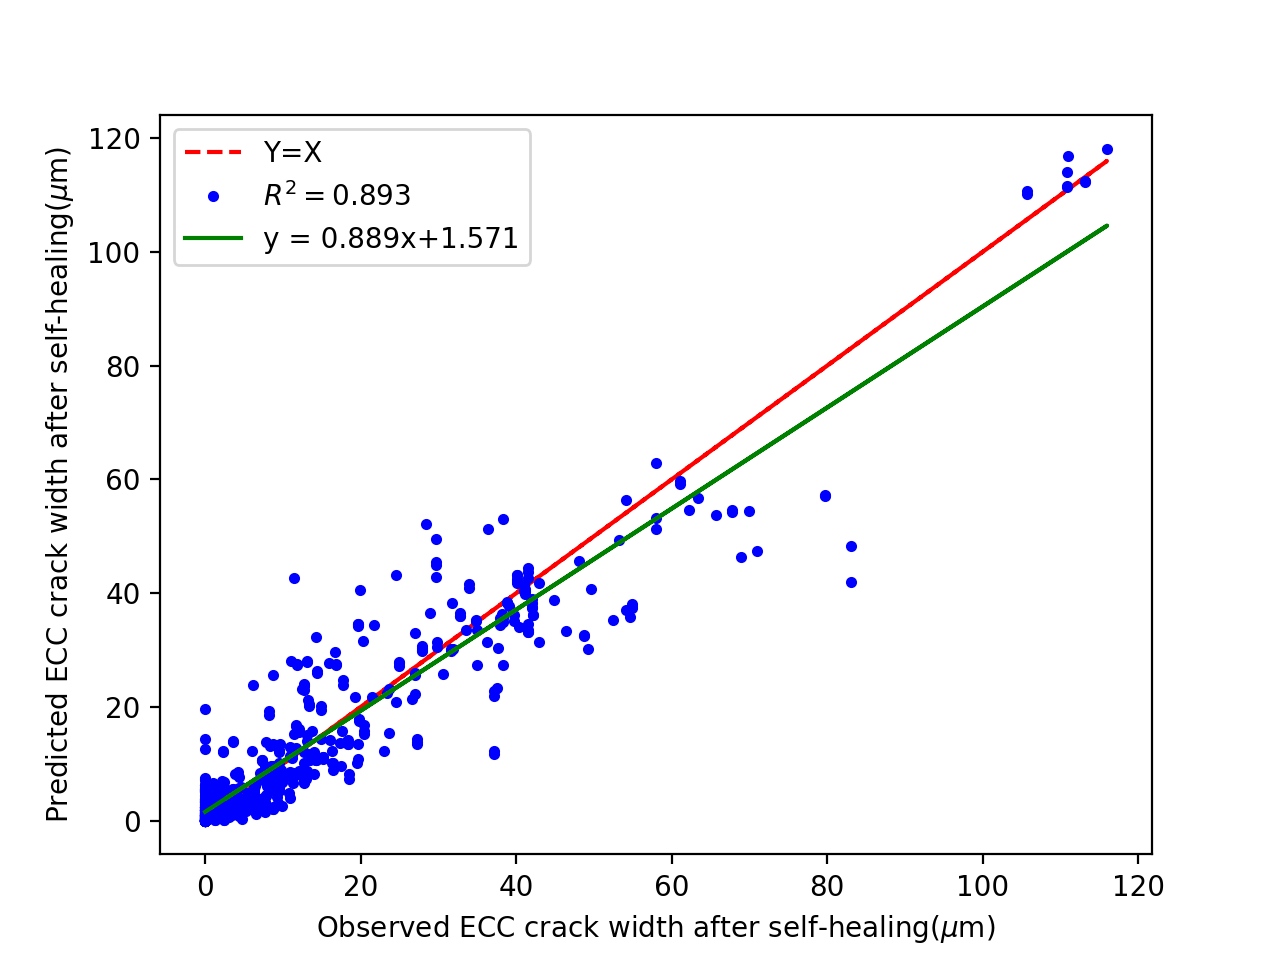
\includegraphics[width = \linewidth]{02Ada_SVR.png}
			\caption{Ada\_SVR}
		    \end{subfigure}%
		\hspace{-1.4em}
		    \begin{subfigure}{.35\textwidth}
			\centering
			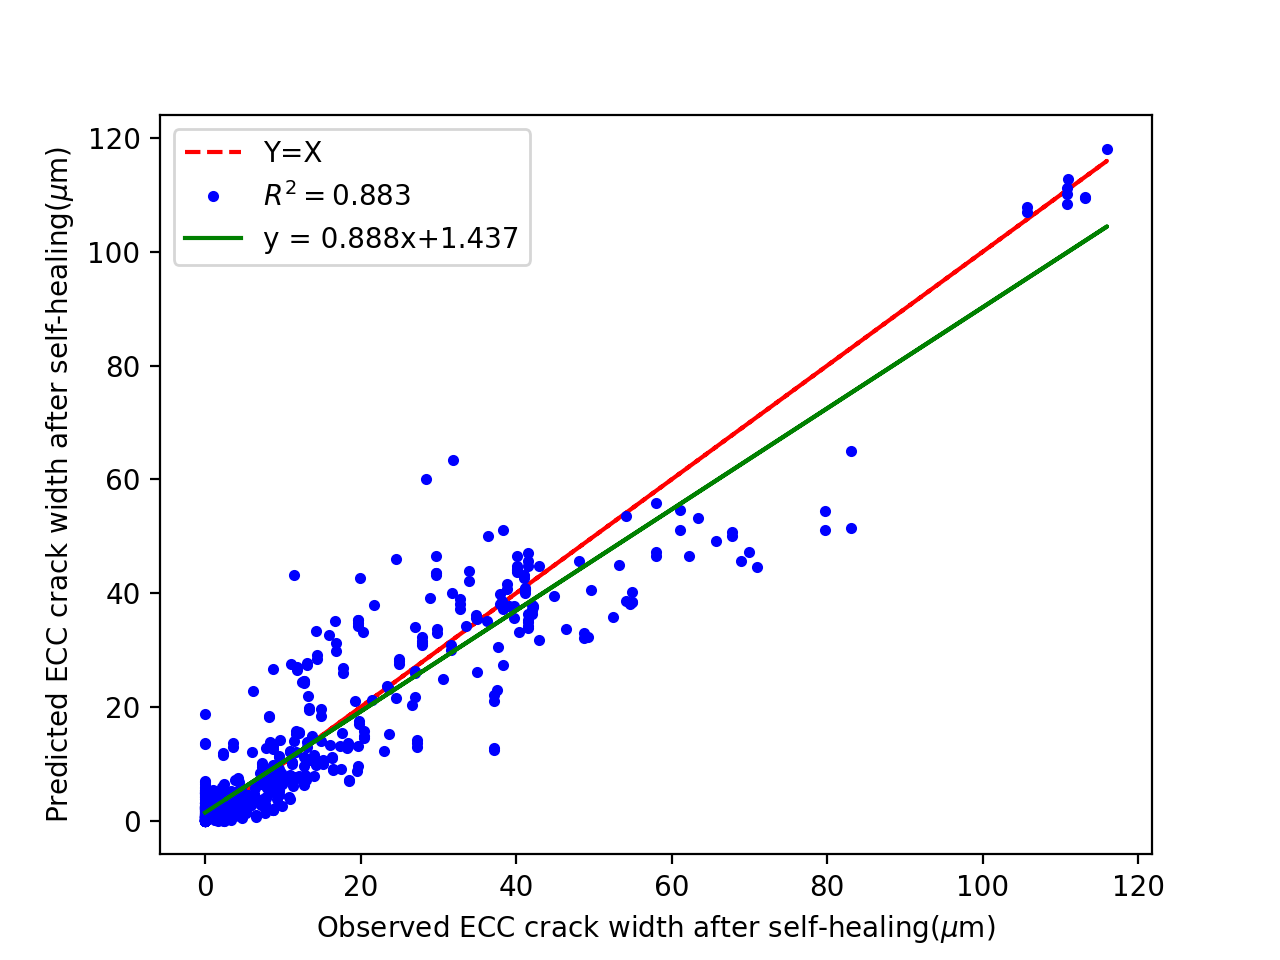
\includegraphics[width = \linewidth]{02Bag_SVR.png}
			\caption{Bag\_SVR}
	    	\end{subfigure}%
		\hspace{-1em}
		\caption{Linear regression of predicted and observed crack width after self-healing of ECC}\label{gbrt}
	\end{figure}
	

	
	It can be seen from Figure \ref{gbrt}(a), for the LR model, the predicted crack width after self-healing has a reasonable performance with the coefficient $R^2$ for 0.860, and the slope $``a"$ of the fit line for 0.799 and the $``y"$ intercept $``b"$ is 3.804. Similarly, as it can be seen in Figure \ref{gbrt}(d), the BPNN model has a better performance than the LR model, which has the coefficient $R^2$ for 0.899, and the slope $``a"$ of the fit line for 0.866 and the $``y"$ intercept $``b"$ is 1.817. And as shown in Figure \ref{gbrt} (a) and (d), the predicted value of crack width after self-healing of ECC in the BPNN model adheres to the target line $Y = X$ better than the LR model, especially for the crack width over 100 $\mu m$, which further indicates the BPNN model is more accuracy and outperform the LR model. Regarding the BPNN, CRAT and SVR model, the SVR model attractively adheres to the target line for the crack width over 100 $\mu m$ after self-healing. And the CRAT model has the best fit line, while the BPNN model has the highest $R^2$ value in either individual models or ensemble models in Figure \ref{gbrt}. That means the slope $``a"$ of the fit line of CRAT model is closer to 1 than other individual models, and of the ensemble models, ada\_CRAT and bag\_CRAT, are closer to 1 than other ensemble models. And the $``y"$ intercept $``b"$ of CRAT model follows the same trends (better than other models). However, the $R^2$ of BPNN is closer to 1 than other individual models, and of ensemble models, ada\_BPNN and bag\_BPNN, are closer to 1 than other ensemble models.  
	
	Specifically, the Stack\_LR model has the best performance with the coefficient $R^2$ for 0.904, and has the slope $``a"$ of the fit line for 0.899 (close to 1) and the $``y"$ intercept $``b"$ is 1.579 (close to 0) as shown in Figure \ref{fig:st}. In addition, as mentioned before, Figures \ref{gbrt} and \ref{fig:st} reveal the experimental data of crack width after self-healing of ECC generated from laboratory experiments is mainly distributed between $0$ to $80 \mu m$. Whereas a few samples have a crack width over $100 \mu m$. This insufficient data may result in machine learning models being trained inadequately and reducing the prediction accuracy.  
	
		\begin{figure}[!h]
	    \centering
	    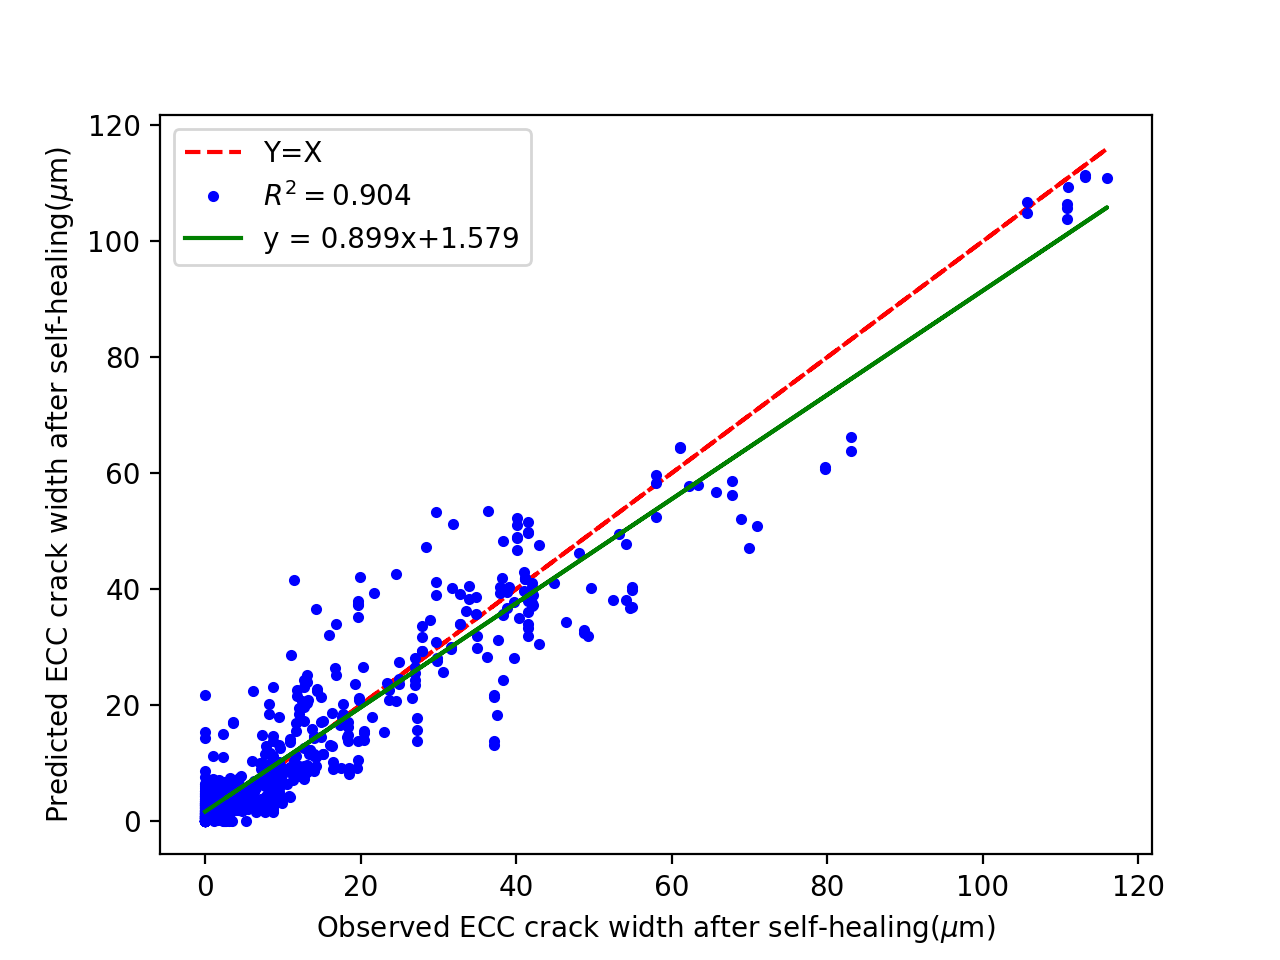
\includegraphics[width = 0.5\linewidth]{02Stack_LR.png}
	    \caption{Linear regression of predicted and observed crack width after self-healing of ECC for stacking ensemble model}
	    \label{fig:st}
	\end{figure}
	
	
% 	In terms of $R^2$, Bag\_CRAT and Bag\_BPNN have the same performance (0.901) and outperform other ensemble methods using an individual method as the base estimator. Moreover, it can be concluded that most machine learning models are able to learn and predict empirical data with an acceptable degree of precision. The performances of all machine learning models described in Table \ref{per} are depicted in Figure \ref{comp} (a), (b), and (c) in terms of MAE, RMSE and $R^2$, respectively.
	
	
% The comparison of the observed and predicted crack width after self-healing of ECC as the self-healing capability of ECC by all machine learning techniques is presented in Figures \ref{gbrt}. For example, plot \textit{(a)} presents the predicted crack width after self-healing of ECC by LR model, which has $R^2$ coefficient for 0.860 and the slope of the straight line for 0.799. As it can be seen, the Stack\_LR has the best performance and obtained a better fit to a straight line with the slope of 0.899 and $R^2$ coefficient of 0.904. In Stack\_LR, the predicted value of crack width after self-healing of ECC adheres to the line ($Y=X$) better than other models, which indicates more accuracy for predicting self-healing of ECC. In addition, Figures \ref{gbrt} reveal the empirical data of crack width after self-healing of ECC generated from laboratory experiments is mainly distributed between $0$ to $80 \mu m$. Whereas a few samples have a crack width over $100 \mu m$.  This insufficient data may result in machine learning models being trained inadequately and reducing the prediction accuracy.  

% 	The comparative analysis of observed and predicted crack width after self-healing of ECC as the self-healing capability of ECC by all machine learning techniques is presented in Figures \ref{f4:lr} to \ref{f4:stack}. 
	

	%%%%%%%%%%%%%%%%%%%%%%%%%%%%%%%%%%%%%%%%%%
%	\begin{figure}[!h]
%		\centering
%		\subfigure[Comparison of observed ECC crack width and predicted ECC crack width after self-healing by LR ]{%
%			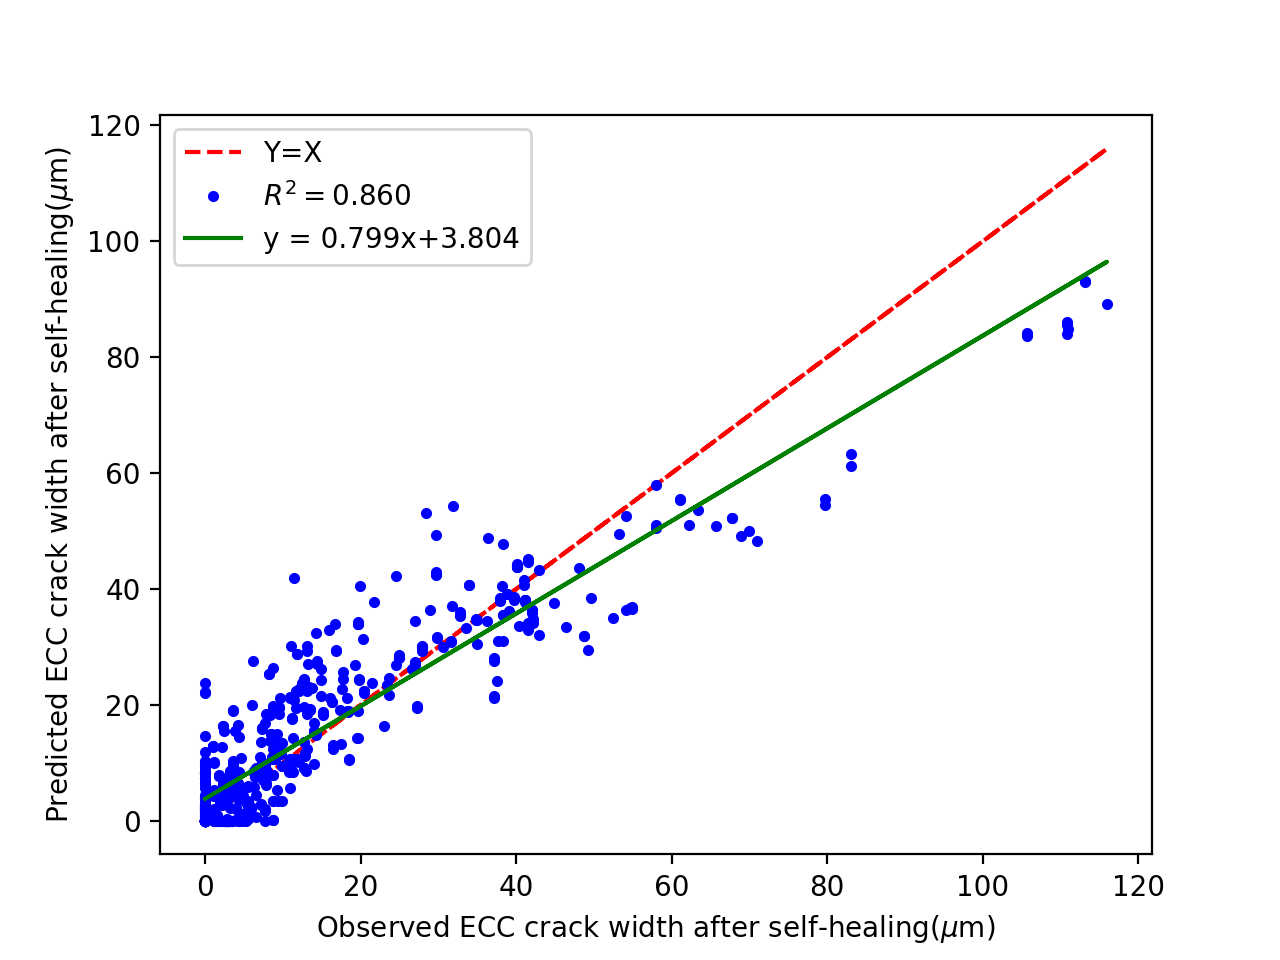
\includegraphics[width=.5\textwidth]{02LR.png}}\hfill
%		\subfigure[Comparison of observed ECC crack width and predicted ECC crack width after self-healing by BPNN ]{%
%			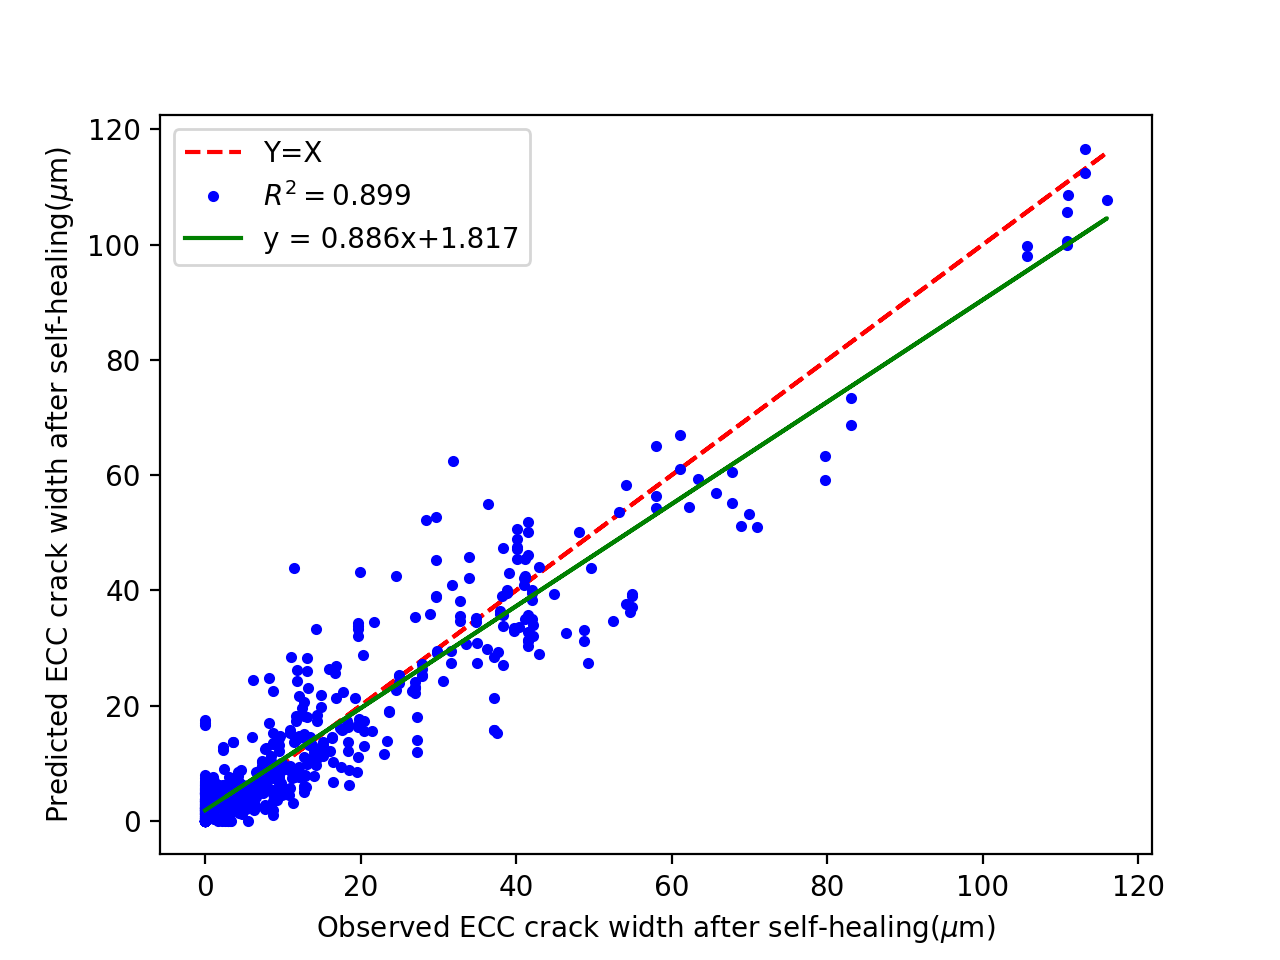
\includegraphics[width=.5\textwidth]{02BPNN.png}}\hfill
%		\subfigure[Comparison of observed ECC crack width and predicted ECC crack width after self-healing by Ada\_BPNN]{%
%			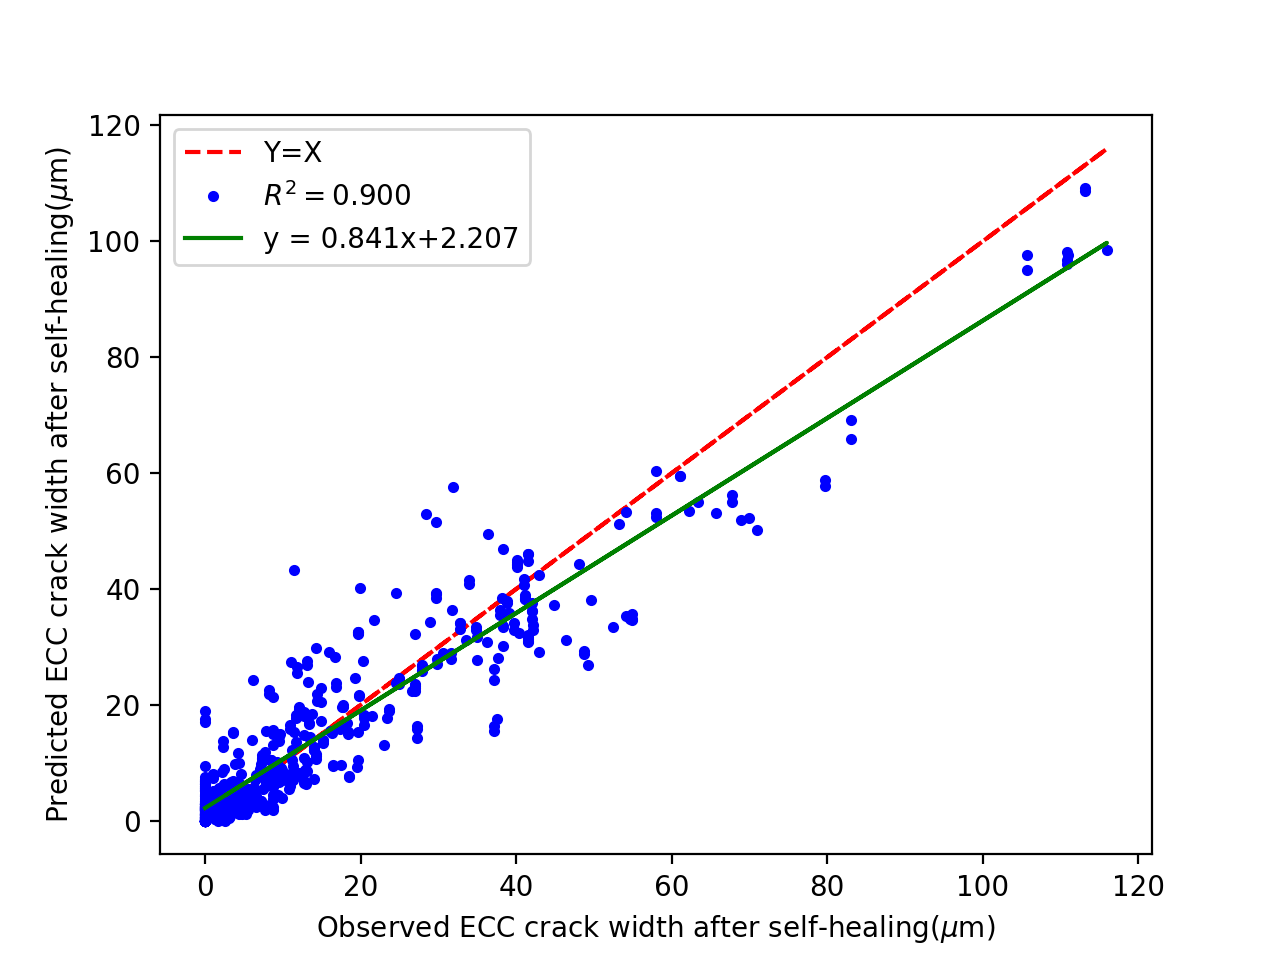
\includegraphics[width=.5\textwidth]{02Ada_BPNN.png}}\hfill
%		\subfigure[Comparison of observed ECC crack width and predicted ECC crack width after self-healing by Bag\_BPNN]{%
%			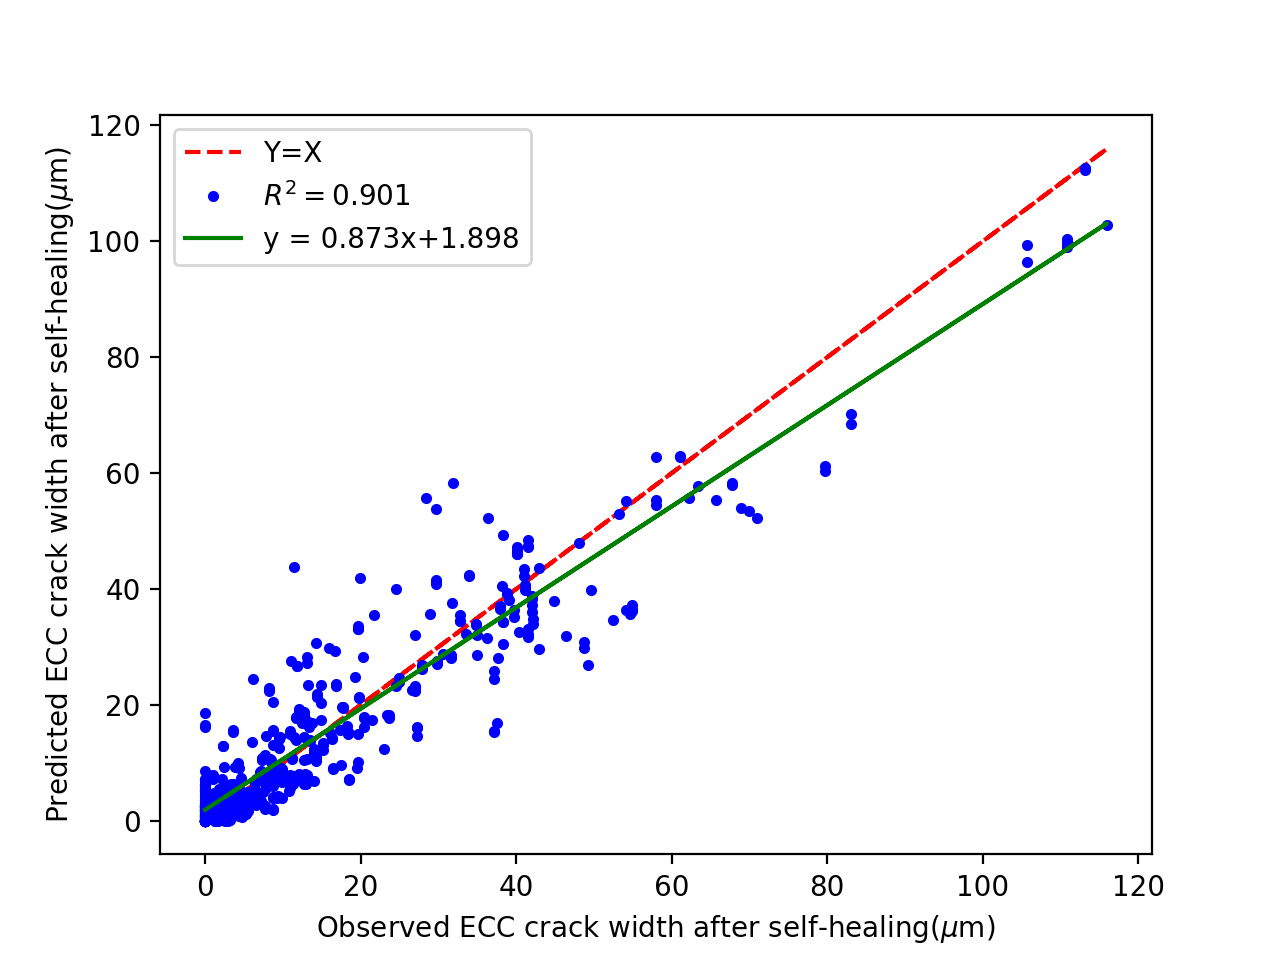
\includegraphics[width=.5\textwidth]{02Bag_BPNN.png}}\hfill
%		\subfigure[Comparison of observed ECC crack width and predicted ECC crack width after self-healing by Stack\_LR ]{%
%			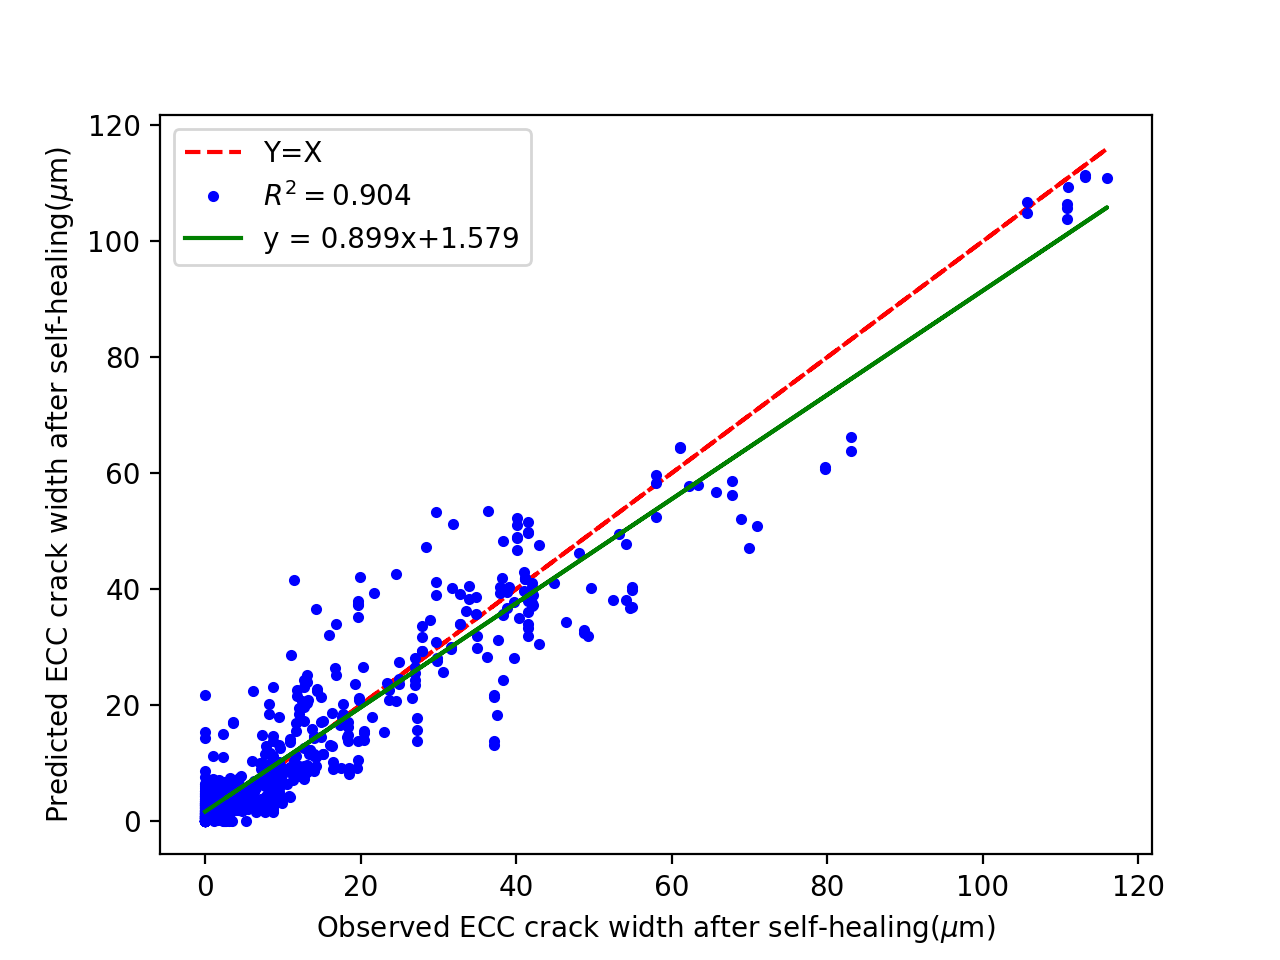
\includegraphics[width=.5\textwidth]{02Stack_LR.png}}\hfill
%		\caption{Comparison of observed ECC crack width and predicted ECC crack width after self-healing by individual and ensemble methods }\label{gbrt}
%	\end{figure}
	
	%%%%%%%%%%%%%%%%%%%%%%%%%%%%%%%%%%%%%%%%%%
	\section{Conclusions}
	\label{con}
	
	This study proposed and compared several individual and ensemble ML models to predict the self-healing ability of ECC. All the proposed ML models were trained, and validated based on the experimental results from nine ECC mixtures. Based on the results, the following conclusions can be drawn.
	
	\begin{enumerate}
	    \item Among of the individual ML model studies, the BPNN model performed the best in terms of RMSE and $R^2$.
	    \item All ensemble methods can generally improve the prediction accuracy of individual methods, however the improvement varies. It is found that Bagging method mainly enhanced the performance of BPNN and CRAT whereas AdaBoost method brought a considerable improvement for LR and SVR models.
	    \item Among all the ML models studies, the Stack\_LR model demonstrated great prediction on self-healing of ECC and performed the best on MAE, RMSE and $R^2$ results. 
	    \item The computational results indicate that the individual and ensemble methods can be used to predict the self-healing ability of ECC. However, how to choose an appropriate base learner and ensemble method is critical. To improve the performance accuracy, researchers should employ different ensemble methods to compare their effectiveness with different ML models. The proposed individual and ensemble ML models can be used to predict the self-healing properties of ECC.
	    \item Future investigation and experimentation should be carried to extend the training dataset to include various crack width distributions and diverse influencing factors such as components, W/MC rate etc.. In addition, more research should be undertaken to optimise parameters in ML models and develop a hybrid model to improve the prediction accuracy.
	\end{enumerate}

	
% 	In this chapter, a comprehensive comparison is proposed to analyse the performance of prediction of the self-healing ability of ECC using individual and ensemble methods. All machine learning models are trained and tested based on the experimental results from nine ECC mixtures. The comparison results provide valuable insights into proposing and validating the machine learning models for predicting self-healing on ECC.
	
% 	A total of four individual methods (LR, BPNN, CRAT, and SVR) and three ensemble methods (bagging, AdaBoost, and stacking) are used to perform the prediction of the self-healing ability of ECC. In these, the performance of LR is used as a benchmark baseline to compare the performance of other individual and ensemble models.  The proposed ensemble methods, bagging and AdaBoost, use one of the four individual methods as a base estimator to aggregate multiple single learning based prediction. The stacking method is used to combine multiple predictions generated by multiple regression models (SVR, BPNN, and CRAT).  
	
% 	The Stack\_LR model demonstrated great predictive ability and the best performance among all individual and ensemble methods, showing the lowest error values on MAE 3.934 and RMSE 6.118 and the highest on $R^2$ 0.904. Moreover, all ensemble methods present the improvement of the predictive ability of individual methods. In particular, the bagging method obviously improves the prediction performance of CRAT on MAE 4.9\%, RMSE 6.6\%, and $R^2$ 1.6\%. On the other hand, the BPNN model performs the best in terms of RMSE and $R^2$ among all individual models.
	
% 	The computational results indicate the individual and ensemble methods can be used to predict the self-healing ability of ECC. However, how to choose a fit base learner for different ensemble methods is critical. Engineers engaged in the design of durable and sustainable ECC mixtures will benefit from the use of machine learning models. Also all individual and ensemble models can be used as a tool for the prediction of the properties of ECC and can be optimized to develop hybrid models for further improving predictive ability.
	
% 	Future investigation and experimentation will be considered to extend the training dataset to include various crack width distributions and diverse influencing factors, such as components, W/MC rate etc., on self-healing of ECC. And more research should be undertaken to explore how to optimize parameters in machine learning models and develop hybrid modelling strategies to improve the prediction accuracy.	
	
	
	
	%next line adds the Bibliography to the contents page
	\addcontentsline{toc}{chapter}{References}
	%uncomment next line to change bibliography name to references
	%\renewcommand{\bibname}{References}
	\bibliographystyle{unsrtnat}  %use the plain bibliography style
	\bibliography{refs}        %use a bibtex bibliography file refs.bib	
	
	
\end{document}